\documentclass[type=bachelor,pifootnote]{thuthesis}
% 选项:
%   type=[bachelor|master|doctor|postdoctor], % 必选
%   secret,                                   % 可选
%   pifootnote,                               % 可选(建议打开)
%   openany|openright,                        % 可选,基本不用
%   arial,                                    % 可选,基本不用
%   arialtoc,                                 % 可选,基本不用
%   arialtitle                                % 可选,基本不用

% 所有其它可能用到的包都统一放到这里了,可以根据自己的实际添加或者删除。
\usepackage{thuthesis}
\usepackage{mathrsfs}
\newcommand\p{\partial}

%code
\usepackage{listings}
%\usepackage{amsmath}
% 定义所有的图片文件在 figures 子目录下
\graphicspath{{figures/}}

% 可以在这里修改配置文件中的定义。导言区可以使用中文。
% \def\myname{薛瑞尼}

\begin{document}

%%% 封面部分
\frontmatter
\thusetup{
  %******************************
  % 注意:
  %   1. 配置里面不要出现空行
  %   2. 不需要的配置信息可以删除
  %******************************
  %
  %=====
  % 秘级
  %=====
  %secretlevel={秘密},
  %secretyear={10},
  %
  %=========
  % 中文信息
  %=========
  ctitle={锂离子电池主要界面力学特性测试和分子模拟研究},
  cdegree={工学学士},
  cdepartment={航天航空学院},
  cmajor={工程力学(钱学森力学班)},
  cauthor={肖飞宇},
  csupervisor={夏勇\quad副研究员},
  %cassosupervisor={陈文光教授}, % 副指导老师
  %ccosupervisor={某某某教授}, % 联合指导老师
  % 日期自动使用当前时间,若需指定按如下方式修改:
  % cdate={超新星纪元},
  %
  % 博士后专有部分
  %cfirstdiscipline={计算机科学与技术},
  %cseconddiscipline={系统结构},
  %postdoctordate={2009年7月——2011年7月},
  %id={编号}, % 可以留空: id={},
  %udc={UDC}, % 可以留空
  %catalognumber={分类号}, % 可以留空
  %
  %=========
  % 英文信息
  %=========
  etitle={The Testing/Characterization and Molecular Simulation of interfaces in Lithium-ion batteries},
  % 这块比较复杂,需要分情况讨论:
  % 1. 学术型硕士
  %    edegree:必须为Master of Arts或Master of Science(注意大小写)
  %             “哲学、文学、历史学、法学、教育学、艺术学门类,公共管理学科
  %              填写Master of Arts,其它填写Master of Science”
  %    emajor:“获得一级学科授权的学科填写一级学科名称,其它填写二级学科名称”
  % 2. 专业型硕士
  %    edegree:“填写专业学位英文名称全称”
  %    emajor:“工程硕士填写工程领域,其它专业学位不填写此项”
  % 3. 学术型博士
  %    edegree:Doctor of Philosophy(注意大小写)
  %    emajor:“获得一级学科授权的学科填写一级学科名称,其它填写二级学科名称”
  % 4. 专业型博士
  %    edegree:“填写专业学位英文名称全称”
  %    emajor:不填写此项
  edegree={Bachelor of Engineering},
  emajor={Mechanics},
  eauthor={Feiyu Xiao},
  esupervisor={Associate Professor Yong Xia},
  %eassosupervisor={Chen Wenguang},
  % 日期自动生成,若需指定按如下方式修改:
  % edate={December, 2005}
  %
  % 关键词用“英文逗号”分割
  ckeywords={电池材料断裂,活性层集流体脱层失效,混合拉伸/剪切加载,弹性常数},
  ekeywords={Fracture of the electrode material, debonding of electrode and substrate, combined tension/shear loading,elastic constants}
}

% 定义中英文摘要和关键字
\begin{cabstract}
研究表明,锂离子电池电极材料的断裂可以造成内部界面的接触失效,引发诸如SEI膜的形成和溶解等连锁反应,从而会进一步造成锂离子电池的性能衰退。同时,电极材料的断裂可能发生在不同的层次和尺度,如晶格、颗粒乃至整个活性层层次。另外,锂离子的脱嵌和嵌入在活性颗粒中产生的应力分布有可能引发颗粒的断裂并进一步在引起宏观上的断裂失效,如颗粒和胶层之间的断裂脱层。这些失效模式十分的复杂,要想对其进行研究和表征,需要考虑不同材料的特性和之间的相互作用乃至考量不同尺度和不同物理场之间的耦合作用。理解电极材料组分之间的界面相互作用,对于防止电极材料的断裂失效有着十分重要的意义。\\
\indent 一方面,在电动汽车的碰撞事故中,车载锂离子电池不可避免地会受到外部力学加载,常常会导致活性层与集流体之间的脱层失效从而引发电池的进一步失效。 实际上,活性层和集流体之前的粘接强度的强弱决定了随着电化学过程进行所产生的内部应力是否会引起内部破坏和失效,另外,粘接强度也显著地影响着接触内阻的大小从而影响着电池的电效率和热效率。 因此,对于活性层-集流体的粘接强度进行力学特征的测试和表征显得尤为重要,而这也将会给锂离子电池的力学建模提供重要的实验参数。\\
\indent 另一方面,在锂离子电池的充放电循环中,锂离子在正负极涂层材料中的脱嵌和嵌入会产生相当大的体积变化,这有可能会导致活性颗粒和粘结剂的脱层失效和电极材料的断裂,从而进一步引起电池容量的下降和电池的老化甚至失效。 从微观上预测和分析锂离子脱嵌和嵌入过程即不同SOC下的活性材料的力学特性对于了解锂离子电池容量消退的微观机理乃至建立多场耦合的预测模型都有着十分深远的意义。\\
\indent 本文将采用一种新的实验方法对集流体-活性层界面粘接强度在混合拉伸/剪切加载下进行直接测试,并研究其动态加载下的应变率效应。 另外,应用DFT计算研究了锂离子在磷酸亚铁锂晶体中的迁移过程并研究其弹性常数在不同SOC下的变化, 应用MD分子模拟的方法研究了锂离子扩散前后其晶体的拉伸-失效力学响应。
从而从宏观力学测试和微观分子模拟的角度对于电极界面强度乃至界面力学、电化学行为进行了全面和深入的研究。

% 工作概述

\end{cabstract}

% 如果习惯关键字跟在摘要文字后面,可以用直接命令来设置,如下:
% \ckeywords{\TeX, \LaTeX, CJK, 模板, 论文}
\begin{eabstract}
Fracture of the electrode material is one of the main degradation
mechanisms in Li-ion batteries, which causes the loss of electric
contact as well as enhances side reactions such as solid electrolyte interface (SEI) formation and dissolution due to the generation of new
interfaces. The electrode fracture may occur at various size scales, including crystals, polycrystals, and aggregates. And the deformation of
active particles can build a stress field in the crystalline
particles, thus
causing fracture at the level of aggregates such as the
debonding of binder and particles. To capture the failure of the constituent materials of the electrode, we must take into account
the mixture of several components with different sizes and properties and the multi-field coupling effect. It is important to understand the interfacial interactions inside the
constituent materials in order to mitigate the undesirable failure.\\
\indent On one hand, the adhesion between electrode and substrate also plays a number of significant roles in battery performance. The quality
of adhesion with the substrate will often dictate whether the electrochemically-induced
strains within the electrode materials are sufficient to cause failure/cracking. In addition,
the adhesion quality between electrode and substrate (which serves as the current collector)
will also influence the contact resistance and, thus electrical efficiency, of the system. Consequently, it is of vital importance to perform he testing and characterization of coating adhesion strength in cathode/anode, and the work will also provide sufficient information to  the mechanical modeling of lithium-ion batteries. \\
\indent  On the other hand, during battery cycling, lithium ions diffuse into and out of cathode/anode materials, causing large volume change. Large volume expansions and contractions in cathode/anode films can cause debonding failure,
significant cracking, capacity loss and degradation or failure. The modeling and predicting of the mechanical properties of active matter in the process of lithium intercalation and deintercalation, namely, different SOCs, is of vital importance, which can help reveal the micro mechanism of capacity fade and establish a multi-physics model.\\
\indent In the present paper, a new test method is proposed to
realize direct measurement of the adhesion strength of the
electrode under a combined tension/shear loading for different
stress states. And the dynamic test considering the loading rate effect is also conducted. Moreover, Li-ion diffusion in $LiFePO_4$ and the elastic constants in different SOCs are studied by first principles density function theroy(DFT) and the mechanical response untill fracture failure of $LiFePO_4$ before and after the Li-ion diffusion is studied via Molecular Dynamics Simulations. In summary, a multi-scale and comprehensive study of the mechanical and electrochemical properties of interfaces in lithium-ion batteries via mechanical testing ways and molecular simulation.
\end{eabstract}


% 如果使用授权说明扫描页,将可选参数中指定为扫描得到的 PDF 文件名,例如:
% \makecover[scan-auth.pdf]
\makecover
\tableofcontents
%% 符号对照表
%\begin{denotation}[3cm]
\item[HPC] 高性能计算 (High Performance Computing)
\item[cluster] 集群
\item[Itanium] 安腾
\item[SMP] 对称多处理
\item[API] 应用程序编程接口
\item[PI] 聚酰亚胺
\item[MPI] 聚酰亚胺模型化合物,N-苯基邻苯酰亚胺
\item[PBI] 聚苯并咪唑
\item[MPBI] 聚苯并咪唑模型化合物,N-苯基苯并咪唑
\item[PY] 聚吡咙
\item[PMDA-BDA]	均苯四酸二酐与联苯四胺合成的聚吡咙薄膜
\item[$\Delta G$] 活化自由能 (Activation Free Energy)
\item[$\chi$] 传输系数 (Transmission Coefficient)
\item[$E$] 能量
\item[$m$] 质量
\item[$c$] 光速
\item[$P$] 概率
\item[$T$] 时间
\item[$v$] 速度
\item[劝学] 君子曰:学不可以已。青,取之于蓝,而青于蓝;冰,水为之,而寒于水。—— 荀况
\end{denotation}



%%% 正文部分
\mainmatter
\chapter{引言}
\section{背景}
近年来,能源危机以及由于能源的不合理运用所带来的环境污染\cite{Goodenough2015Energy}等问题已经越来越成为制约着人类经济社会发展的关键因素。
在针对这一核心问题的诸多探索和尝试中,寻求一种可以足够安全地储存能量并能相对容易和高效地将储存的能量转换为电能的方式和器件尤为重要\cite{Feng2017Thermal}。同时,在方兴未艾的汽车电动化和新兴的自动驾驶等技术的发展浪潮中,汽车的能源储备系统正在经历着从化石能源到电化学能源\cite{Shan2016The,Tarascon2001Issues,Dunn2011Electrical}的广泛和深刻的变革。 而在这场变革中,锂离子电池系统由于有着高能量密度,使用寿命长乃至对环境相对友好的优点得到了广泛的应用\cite{Yoshio2003Spherical,Taberna2006High}并被赋予深厚的希望。 实际上,我们正在迅速接近车辆电动化的临界点,主要的汽车生产商都制定了雄心勃勃的各系列电动汽车的生产计划。 根据国际能源组织的统计,到2025年,全世界的电动汽车的保有量将达到一亿辆\cite{plan}。 巨大的市场和行业的迅速成长所带来的对车载电池的能量密度增长和对于电池成本降低的迫切需求,都带来了整个社会对于电动汽车安全性方面的担忧\cite{Zhu2018A}。\\
\indent考虑到每年电动汽车的巨额销量和迅速增长的保有量,可以预料到,这些车辆会不可避免地遭遇汽车碰撞事故,而在碰撞事故中,其电池系统会经历很多频繁的侵入或者冲击加载\cite{Xu2016Computational}。 同时,电池能量密度的提升和电动汽车对里程数的增加要求必然也会导致在相同的情况下电池受损造成的后果愈加严重。 实际上近几年,锂离子电池的故障导致的一些电动汽车的火灾和爆炸事件屡见报端\cite{volt,BYD,boeing,Tesla}(见图[\ref{fig:accident}]),造成了愈演愈烈的对于车载电池安全性的担忧。
\begin{figure}
\centering   
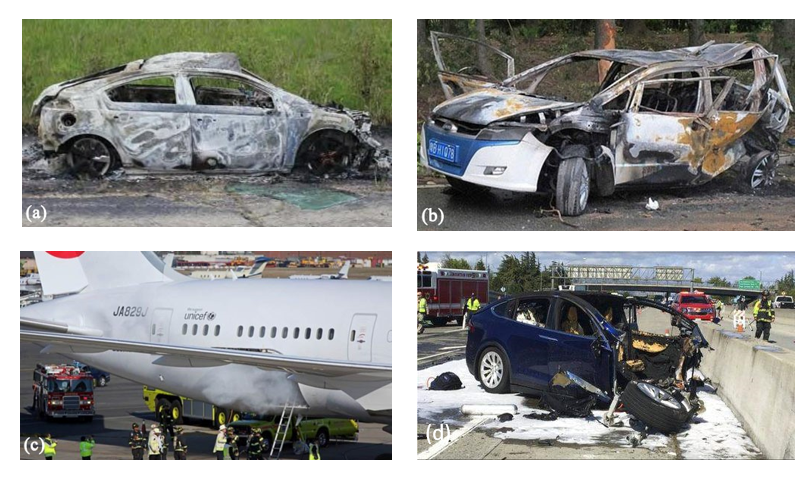
\includegraphics[width=\textwidth]{accident.png}
\caption{锂离子动力电池火灾:(a) Chevrolet Volt (b) BYD e6 (c) Boeing 787 (d) Tesla Model X } 
\label{fig:accident}
\end{figure}
\\
\indent 到目前为止,在所有会造成电池失效的因素如,制造缺陷、过充和过放\cite{Kermani2017Review}中,机械滥用是其中十分重要但是尚未得到充分研究和深刻理解的因素。 长期以来,对于锂离子电池的研究大多数都集中在对于其内部电化学过程的研究,对于其机械失效的研究十分稀少。而实际上,在碰撞事故中,电动汽车的车载电池包将有很大可能受到复杂外载从而产生变形,而这可能引起电池的内短路进一步发展成热失效从而引起诸如着火和爆炸等严重后果。 举例而言,内短路会由于机械外载造成的电池接头的外部保护失效从而导致正极和负极接触而产生。 由此可见,对于电池组分乃至结构单体到模组的力学性质和变形响应的定量探究和理解十分重要。\\
\indent 锂离子电池的力学失效特性和进一步所引发的热失效的整个过程有着多尺度,多物理场、非线性的特点,使得对于其的研究有很大的困难。一般而言,对于锂离子电池的力学失效特性的研究主要按照研究尺度和测试条件展开。 首先,最小的层次是晶体和颗粒层次,在这一层次往往可以研究电化学和力学行为的耦合特性,有着一系列的微观测试和模拟计算的方法。 在这一尺度,研究者对于电极体积的脱锂和嵌锂的变化,活性颗粒的变形和开裂,力学外载造成的电极材料性能衰退,内部应力分布乃至固体电解质膜的形成及其力学电学特性\cite{Behrou2017Multiscale,Behrou2017Numerical,Zhao2012Fracture,Zhao2010Fracture}进行了研究。 其次,相当多的研究对于电池的组成成分如电极、隔膜在不同力学外载下的力学响应\cite{Cannarella2014Mechanical,Zhang2016Li,Kalnaus2017Mechanical,Sheidaei2011Mechanical}进行了测试和建模。 另外还有对于电池的单体的诸多测试和力学建模的均质化模型和精细模型的研究\cite{Elham2012Calibration,Greve2012Mechanical,Sahraei2012Modeling,Sahraei2014Characterizing},乃至模组和系统层次的研究\cite{Ali2015Computational,Wang2017Progressive,Xia2014Damage,Kukreja2016Crash}。 
表\ref{tab:component}展示了对于锂离子电池的组分力学测试的研究和相关结果。
\begin{table}
    \centering
    \caption{重复单元组分及其力学性质}
    \label{tab:component}
    \begin{tabular}{ | c | p{1.8cm} | p{1.8cm} | p{0.5cm}|}
    \hline
    组分 & 材料 & 力学响应 & 参考文献 \\ \hline
    集流体 & 铝箔/铜箔 & 各向同性 应变硬化 塑性断裂 应变率响应 & \cite{Sahraei2016Microscale} \quad \quad  \cite{Sahraei2015Modelling} \quad \quad \cite{Greve2012Mechanical} \quad \quad \cite{Luo2015Fracture} \\
    涂层 & 石墨颗粒/活性物质颗粒 & 压力相关 & \cite{Dass} \\
    隔膜 & 多孔有机物 & 各向异性 粘弹塑性 温度相关  &  \cite{Huang2011Separator} \quad \quad \cite{Lee2014A} \quad \quad \cite{Zhang2016Deformation} \\ \hline
    \end{tabular}
\end{table}
\section{锂离子电池力学性质研究现状}
前文已经指出,在电动汽车的碰撞事故中,如果电池包产生结构损伤、分裂就有可能发生电池的热失控并引起火灾甚至爆炸。 为了对车载锂离子电池进行安全防护的研究和设计,需要对其力学外载响应和电化学-力学耦合响应有一个清晰的认识和理解,而这其中涉及了多尺度、多物理场的复杂问题(见图\ref{fig:zhu})。\\
\begin{figure}
\centering   
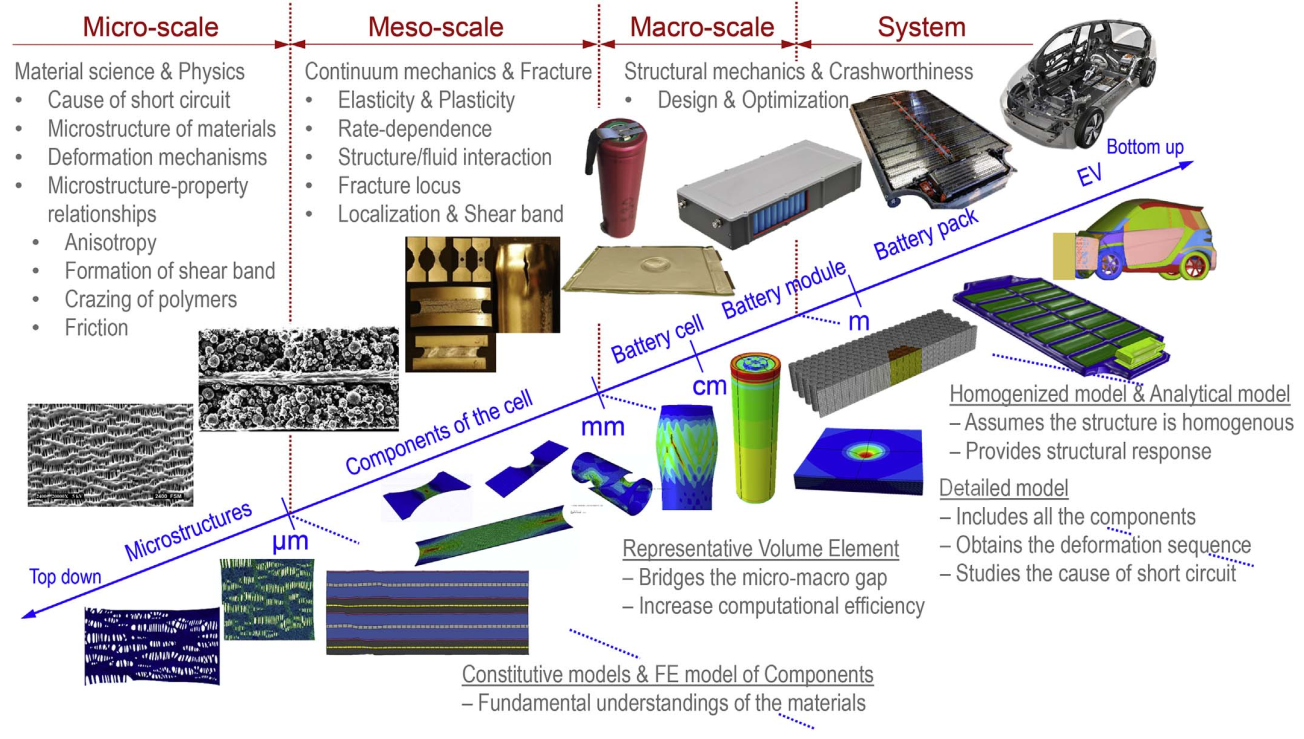
\includegraphics[width=\textwidth]{zhu.png}
\caption{锂离子电池力学性质研究涉及多个尺度和层面}
\label{fig:zhu}
\end{figure}
\indent 在介绍本文的研究内容之前,首先有必要对于锂离子电池的构成和组分进行简要介绍并对之前的对于组分力学性质的研究做一个归纳和总结。\\
\begin{figure}
\centering   
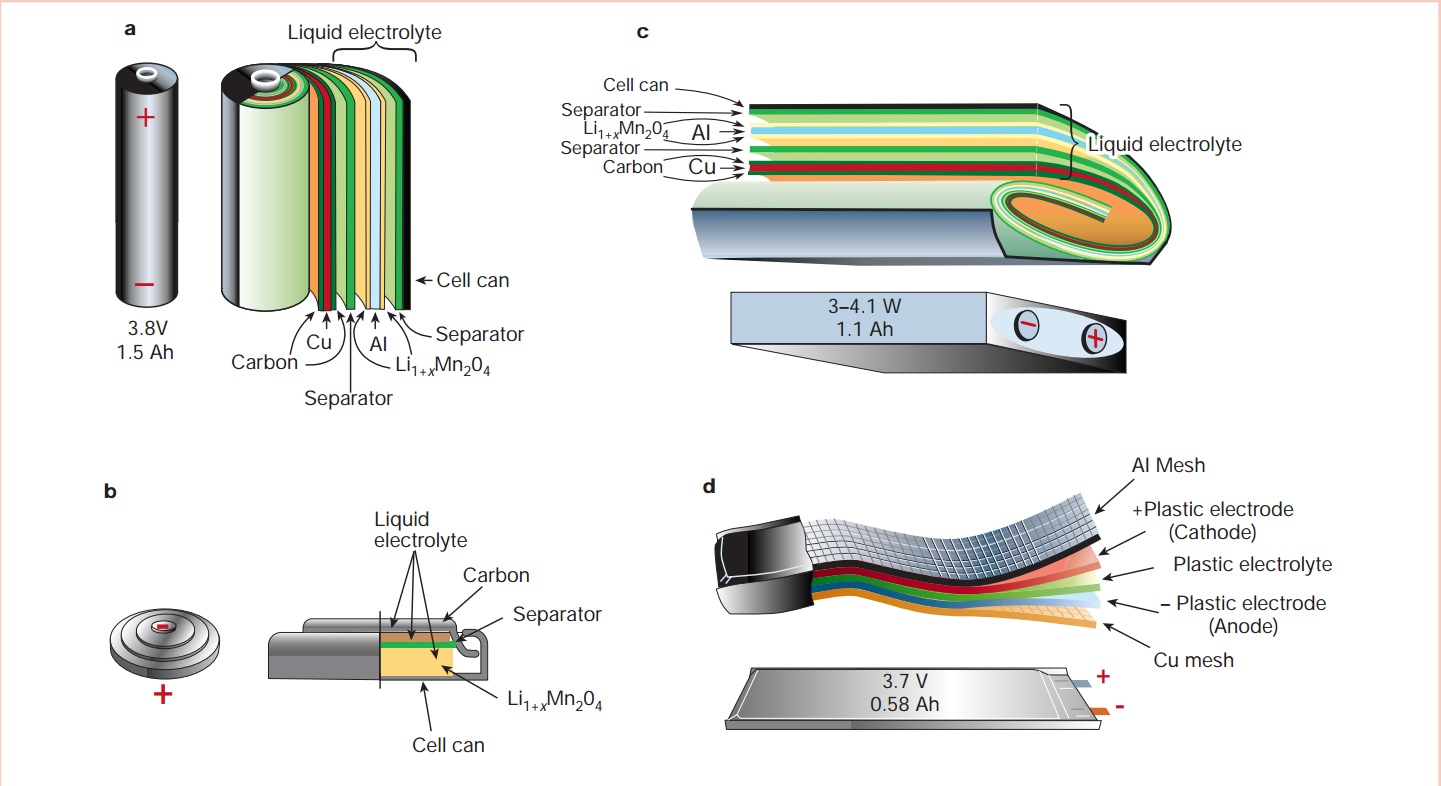
\includegraphics[width=\textwidth]{battery.png}
\caption{各种锂离子电池的形状和组成的示意图\cite{Tarascon2001Issues}:(a)圆柱形 (b)方形 (c)纽扣形 (d)软包形}
\label{fig:battery}
\end{figure}
\indent 锂离子电池作为一种典型的二次电池,其工作原理是依靠锂离子在电池的正极和负极的嵌入和脱嵌来传递电流。 其典型的类型按照形状来划分有圆柱型(如18650)、方形、纽扣形和软包形(图\ref{fig:battery})。 就微观和介观结构而言,商用车载锂离子电池通常采用多层电极堆叠的结构(见图(\ref{fig:structure}a)),其每一个重复单元由正极、负极和隔膜组成。 更细致而言,正极是由两侧涂布有活性物质层的铝箔组成,类似地,负极是由两侧涂布着石墨或者硅颗粒的铜箔组成。 这些成分都浸润在电解液中并被钢壳或者铝塑膜覆盖密封。 在电子显微镜下可以清晰分辨出正极和负极的三明治结构和隔膜的多孔结构(见图(\ref{fig:structure}b-d))。
\begin{figure}
\centering   
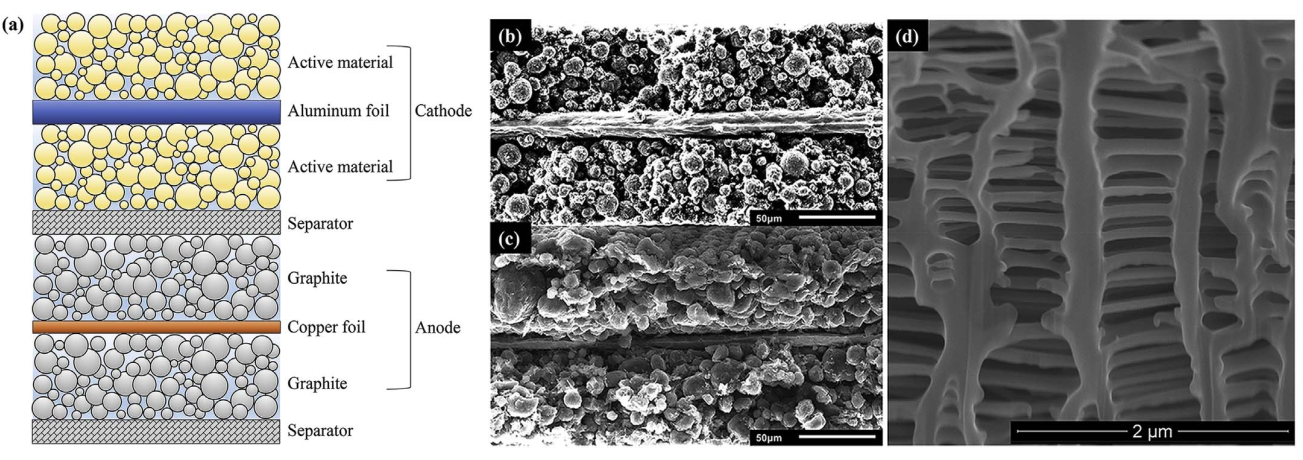
\includegraphics[width=\textwidth]{structure.png}
\caption{(a)锂离子电池的重复单元和组分的截面图 (b)正极 (c)负极 (d)隔膜}
\label{fig:structure}
\end{figure}
\section{研究目标}
对当前的电动汽车产业而言,如何在保证其安全性和可靠性的前提下设计出有着更高能量密度和更长寿命周期的电池至关重要。 为了实现这个目标,开展了大量关于电极活性材料的研究\cite{Cheng2011Functional,Park2015LiFeO2},然而,其中少有涉及到对于活性层和集流体的胶接强度的研究,而实际上保证足够的胶接强度无论对于充放电循环的实现和电池寿命的保证还是对于安全防护都至关重要\cite{Chen2013Unveiling}。\\
\indent 一方面电池周期性的充放电循环会产生交替的内应力,可能会导致活性物质内部裂纹的产生甚至活性层和集流体的分层这些不可逆的变化,从而可能导致电池容量的减小和循环次数的减少\cite{Vetter2005Ageing}。 研究表明,对于硅-锡电池系统(其在锂离子脱嵌和嵌入过程中的体积变化可以高达250\%)而言,即使其活性颗粒在体积膨胀和收缩的过程中不发生断裂,依然会发生活性颗粒之前的电接触条件变差(接触面减小或者脱离接触)导致容量减小\cite{Chen2003A,Chen2003Large}。 所以,为了保证一个良好的电池生命周期,在活性物质和集流体之间维持良好的连接条件显得至关重要。
\begin{figure}
\centering   
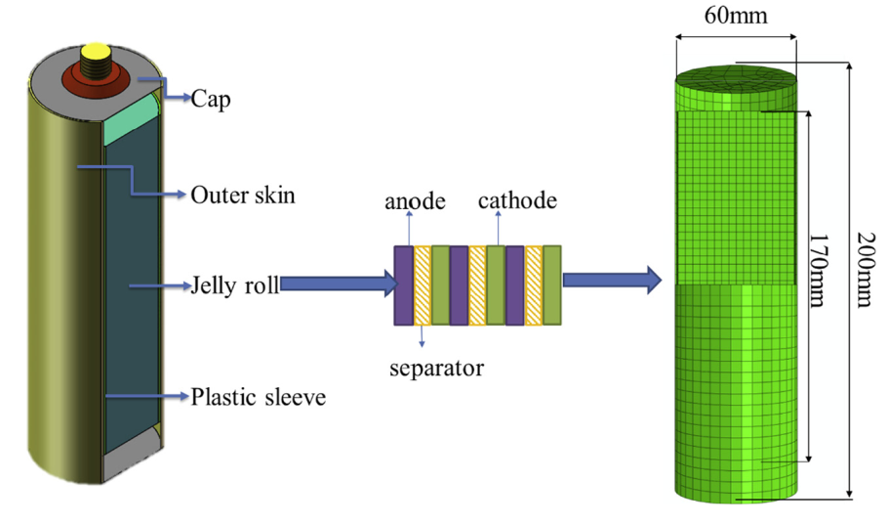
\includegraphics[width=0.8\textwidth]{homo.png}
\caption{HP 602030电池的均质化有限元模型}
\label{fig:homo}
\end{figure}\\
\indent 另一方面,为了准确的表征电动汽车的碰撞工况和车载电池的碰撞响应,需要建立准确的有限元模型。 起初建立的模型大多是均质化的有限元模型,在这些模型中,整个电池单体被看做是同种材料进行建模(见图(\ref{fig:homo})),但是实际的碰撞工况往往涉及大变形和多种形式的动态加载,使得简单的均质化建模难以准确预测电池在碰撞事故中的失效行为\cite{Luo2018Adhesion}。 随着对于电池组分材料力学行为的测试和表征,基于这些数据建立精细化的有限元模型有望相对准确地分析和预测电池的碰撞失效演变行为\cite{Lu2013A}。 而在电池组分水平,其多层结构中的界面力学特性,如活性层粘接强度,尚未得到充分的研究,而在力学有限元建模中界面力学特性会明显影响电池在外部加载下的局部和总体的力学响应。\\
\indent 同时,前文也指出,对于电池力学性质的研究往往很少考虑电化学因素的影响,而对于锂离子电化学性能的研究却也很少包括对于力学特性的表征。 而本文所关注的锂离子电池活性层-集流体界面强度的研究必然包括着对于锂离子扩散过程的考量,也就意味着如果想要建立一个全面的模型必须要同时对于力学和电化学因素进行综合考虑。\\
\indent 总结而言,对于锂离子电池界面力学性质的测试和表征是一项有意义和有挑战的工作,尤其是探究其在混合加载和动态加载等接近实际工况下的力学响应。 本研究的目的在于直接测定集流体和活性层在混合力学加载下的的粘接强度,从而为精细化的力学建模提供模型参数的支持以及为预测界面脱层失效乃至电池失效响应提供实验支持。另外本研究将利用分子模拟的手段从微观层面对于颗粒在锂离子脱嵌和嵌入过程这一锂离子电池循环周期中关键的电化学过程中的颗粒的力学特性乃至其断裂特征进行研究,从而补充和佐证界面力学测试实验,并为进一步的耦合研究提供基础。
\section{文章架构}
本文第2章将探讨界面力学实验方案的设计,首先将介绍现有研究方法的特点和不足,进而对于胶接作用中断裂失效的可能模式进行了分类,提出一种获得给定的活性层-集流体界面脱层失效模态的实验方法。 另外将介绍实验的准备工作,包括对于实验方法的验证分析以及对于在后续分析中所会用到的断裂准则和内聚力模型进行了介绍。 \\
\indent
第3章在第2章的基础上讨论和分析了电池正极和负极的静态和动态实验的测试结果,并给出了包括了电化学影响的颗粒-壳体模型来在微观层面进行力学表征。 \\
\indent 第4章首先利用第一性原理计算的方法计算出了$Li$离子在$LiFePO_4$晶体中沿着两个不同方向进行扩散的能垒和反应活性并得到了主要扩散方向上进行扩散时的扩散路径, 接下来基于此同样采用第一性原理计算的方法对于其在$Li$离子扩散过程中晶体的弹性常数及相应力学参数的变化进行了研究,同时也讨论了其力学各向异性;最后利用分子动力学计算的方法对于$Li$离子扩散前后的$LiFePO_4$晶体进行应变加载,并在模拟中成功观察到了其断裂失效行为。 \\
\indent
第5章对于全文结果进行了总结分析,并提出了对接下来可能进行的工作的展望。
\chapter{界面粘接强度试验设计}
\section{研究现状和研究设计}
\subsection{电极活性层-集流体相关胶接作用研究}
基于之前对于锂离子电池电极内部结构(\ref{fig:structure})的介绍,进一步的说,无论是正极还是负极,除了活性颗粒之外内部还掺杂着导电剂和粘结剂,而后者在各个成分的粘接中发挥了至关重要的作用。 实际上,活性层和集流体之前的连接的建立也是依靠着内部的粘结剂而形成\cite{Haselrieder2015Measuring}。
在电极活性材料的制备和其涂布的过程中,由于活性层内部材料组成成分的多样、活性颗粒的形状大小不一等因素,以及粘结剂会和活性物质相互作用\cite{Liu2012Particles}而产生重新分布造成复杂的内部结构\cite{Lee2007A,Stevenson2008The},都使得对于活性层的力学特性的研究面临着相当大的困难\cite{Yoo2003Effect}。\\
\indent 总之,在电池的工作循环中,颗粒之间,颗粒和集流体之间的粘接强度对于保证电极的力学完整性乃至电化学功能有着十分重要的作用。 已经有研究表明,这一粘接强度对于电极的电流传导\cite{Chen2003Comparison}和电池的容量保持\cite{Lee2006Effect}都有着相当大的影响。 而更加重要的是,在前文已经指出,对于高容量的电池而言,其电极材料往往会由于可以容纳更多的Li离子从而会产生更大的体积变化,此时胶接强度就显得更加重要。因此,有必要对于电极的胶接强度特性进行完整的力学测试和建模,从而指导电极的设计和优化。 另外,对于电动汽车在碰撞事故过程的分析中,需要对电池包进行冲击工况的建模,此时界面的粘接强度的一系列力学参数都需要实验予以标定和整合。
\subsection{胶接作用影响因素}
活性层和集流体的粘接强度受着多种因素影响,由电极的内部结构所决定\cite{Seki2004Effect,Jing2008Effect},取决于电极中不同颗粒之间以及颗粒和集流体之前的物理吸附和化学键合的特性。 通常而言,粘接强度取决于活性物质之间的接触和粘接乃至活性物质和基底(即构成集流体的金属箔)之前的粘接,从而活性颗粒的尺寸大小颗粒之前形成的接触的种类和个数都主导着胶接强度的大小\cite{Kwade}。 而之前的研究已经从诸如其组成材料\cite{Yoo2003Effect,Chen2006Binder,Liu2005Enhanced}(活性颗粒、金属箔和粘接剂)之间的物理化学的界面相互作用、电极的组成结构\cite{Buqa2006Study,Liu2012Particles,Stevenson2008The}乃至电极的生产过程\cite{Lee2007A,Jing2008Effect,Park2007Mechanical}等不同尺度和角度展开。接下来将首先对于之前的研究胶接强度的研究进行简要综述,再介绍本文所设计和采用的研究方法。
\begin{figure}
\centering   
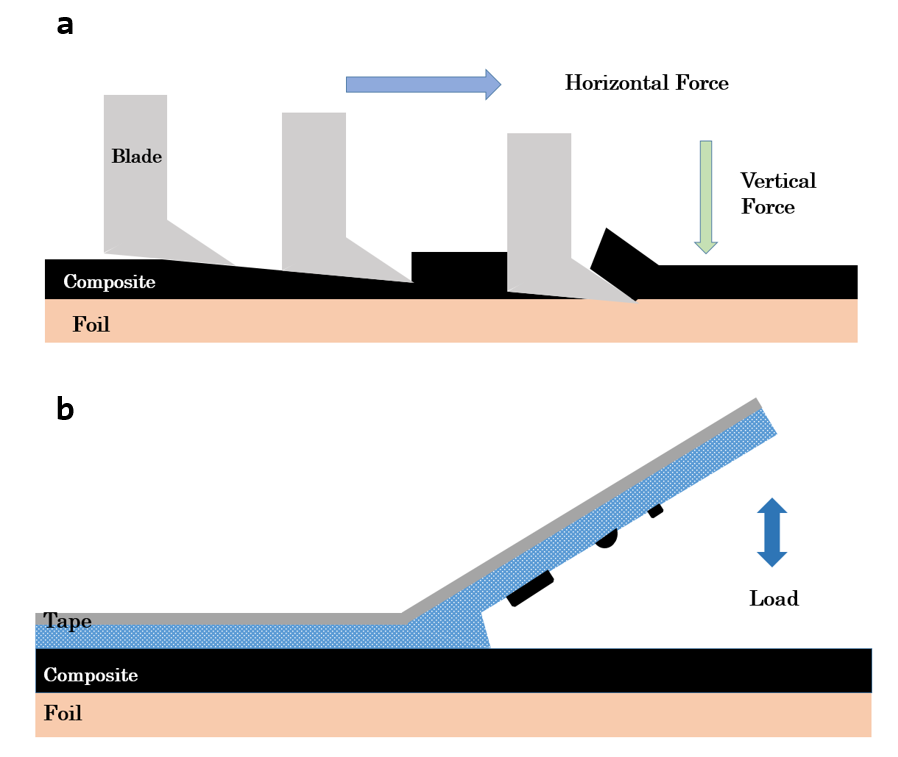
\includegraphics[width=\textwidth]{previoustest.png}
\caption{对活性层界面强度的测试方法:(a)SAICAS测试(纳米压痕法) (b)传统的Peel测试} 
\label{fig:pretest}
\end{figure}
\subsubsection{胶接强度试验方法调研}
之前的强度测试主要有两种方法,如图\ref{fig:pretest}所示。 Peel测试(见图\ref{fig:pretest}(a))实际上是使用胶带从集流体上利用黏性将活性物质粘离,从而得到测试界面强度的数据。由于该测试方法操作简便,能大致估算出界面强度,所以在工业界得到了广泛应用。比如之间有研究用这一方法来测量活性层和金属薄膜基底之前的粘结强度,并探究了诸如悬浮工艺(在负极生产中采用)对于电极强度的影响\cite{Park2011Effect}。 但是,这一操作相对简单的方法的测试结果十分受到诸如使用的胶带的种类,胶带和测试样品的起初的粘接强度等因素的影响。 另外,Peel测试中,几乎所有的断裂都发生在活性层的较浅的表层,所以其测得的粘接强度是表面的而不是整个体材料的,更不用说几乎无法测得活性层和集流体的粘接强度。 也就是说,通过Peel测试得到的粘接强度所对应的失效位置是难以确定的并且也无法得到活性层-集流体界面的粘接强度这一在建模中十分重要的参数。\\
\indent 另外一种方法是利用纳米压痕的方法测定给定深度和位置的粘接强度(SAICAS\cite{Son2014Measurement}),这一方法同时也可以用于对电极断裂的演变的研究\cite{Saito2010An}。 但是其测试结果很难被直接转化为活性层-集流体的粘接强度,而且并不能研究复杂加载乃至动态加载的力学响应行为。\\
\indent 接下来将介绍所设计的一种可以在混合拉伸-剪切工况下测量电极活性层-集流体粘接强度的测试方法,这一测试方法同时也可以很好的进行不同应变率加载的测试。 本章将首先介绍实验方法的详细设计和实验分析所会用到的断裂准则和材料模型,对于具体电极(包括正负极在不同角度加载实验和动态实验)的实验结果及其分析将在第三章详细说明。
\subsection{实验方法设计}
\subsubsection{试样设计}
在试验中,所研究的对象是活性层-集流体-活性层这样的三明治结构,即由两侧的多孔的活性物质粘附在中间的金属薄膜上构成。 考虑到整个电极的纵向厚度不超过200$\mu m$,所以很难对这一结构施加直接的边界约束从而展开力学测试。 所以在实验中,将活性层的两侧通过胶水粘附到两侧的基底上再对试样固定到夹具上进行实验,如图\ref{fig:specimen}所示。
\begin{figure}
\centering   
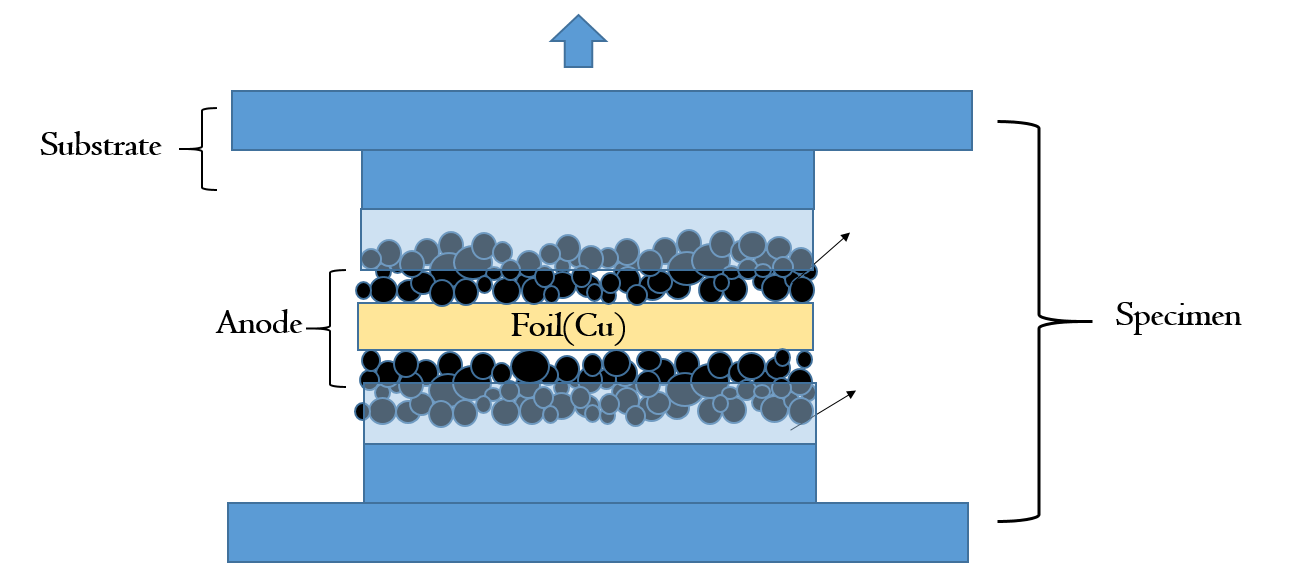
\includegraphics[width=\textwidth]{Specimen.png}
\caption{试样的结构示意图} 
\label{fig:specimen}
\end{figure}
\\
\indent 由于所研究的结构为一个多种物质构成的多层次结构,所以显而易见,在力学加载过程中,其可能发生的断裂失效模式有三种,如图\ref{fig:mode}所示。 失效分为,基底和活性层之间的断裂(这可以通过使用强度合适的胶水和改进涂布方法得到避免),活性层内部的断裂失效(这也称为内聚失效)和活性层和集流体之前的脱层失效(即粘接失效)。由于实验的测定目的为研究活性层和集流体之前的脱层失效,则希望力学测试中失效行为都为第三种失效,即断裂都发生在活性层和集流体之间。
\begin{figure}
\centering   
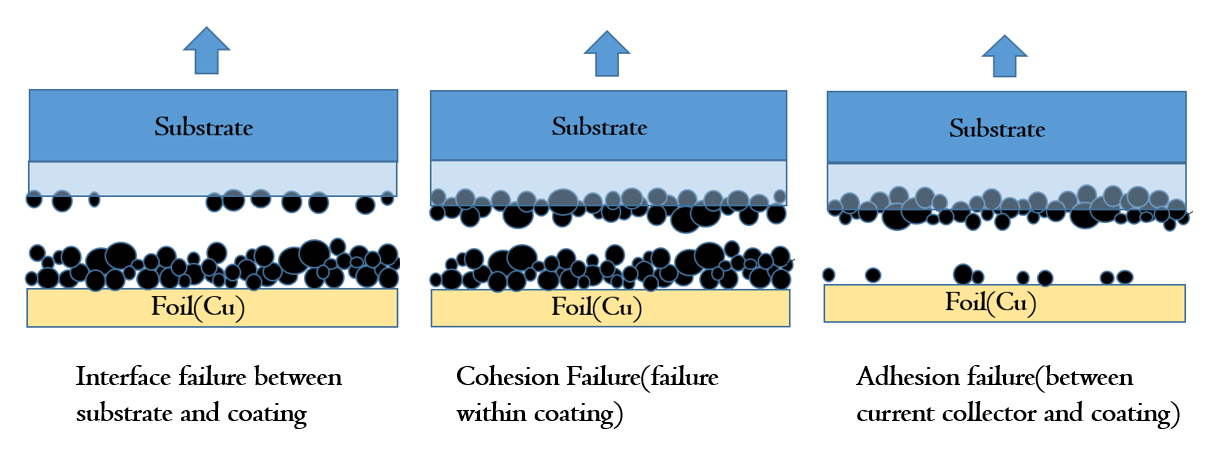
\includegraphics[width=\textwidth]{failuremode.png}
\caption{不同的断裂失效模式: 基底和活性层之间的断裂, 活性层内部的断裂和活性层和集流体之间的断裂} 
\label{fig:mode}
\end{figure}
\\
\indent 为了达成这一目的,将一侧用渗透性很强的胶水代替,从而能使得第一种断裂很难发生;另外,研究表明,由于活性层的涂布工艺,内部粘结剂的含量从外侧到集流体侧逐渐减小\cite{M2017Investigation},使得第二种失效相对第三种失效不易发生,从而只需要考虑另外一侧(即图中加载侧)的断裂。 而在实际的试验中,在下侧使用液体万能胶(Super Glue 15187)粘接,而上侧选用了特殊的凝胶(Loctite Super Glue)粘接,从而可以保证失效只在上侧发生并主要是第三种失效模态。(见图\ref{fig:geltype})。在液体胶侧,液体胶很容易整个渗透入活性层的多孔结构中,这会大大增强其力学强度并且这一侧的集流体-活性层界面也会被加强。 而另外一侧,凝胶由于其很差的渗透性只在表面的很少部分粘接(后续部分会有具体的实验测定),从而不会影响到起初的这一侧的集流体-活性层的粘接。 通过这样的试样处理和制备,只有凝胶侧的集流体-活性层的粘接强度相对最低,从而在力学加载中最容易发生失效,从而就可以得到起初所希望得到的失效模式。
\begin{figure}
\centering   
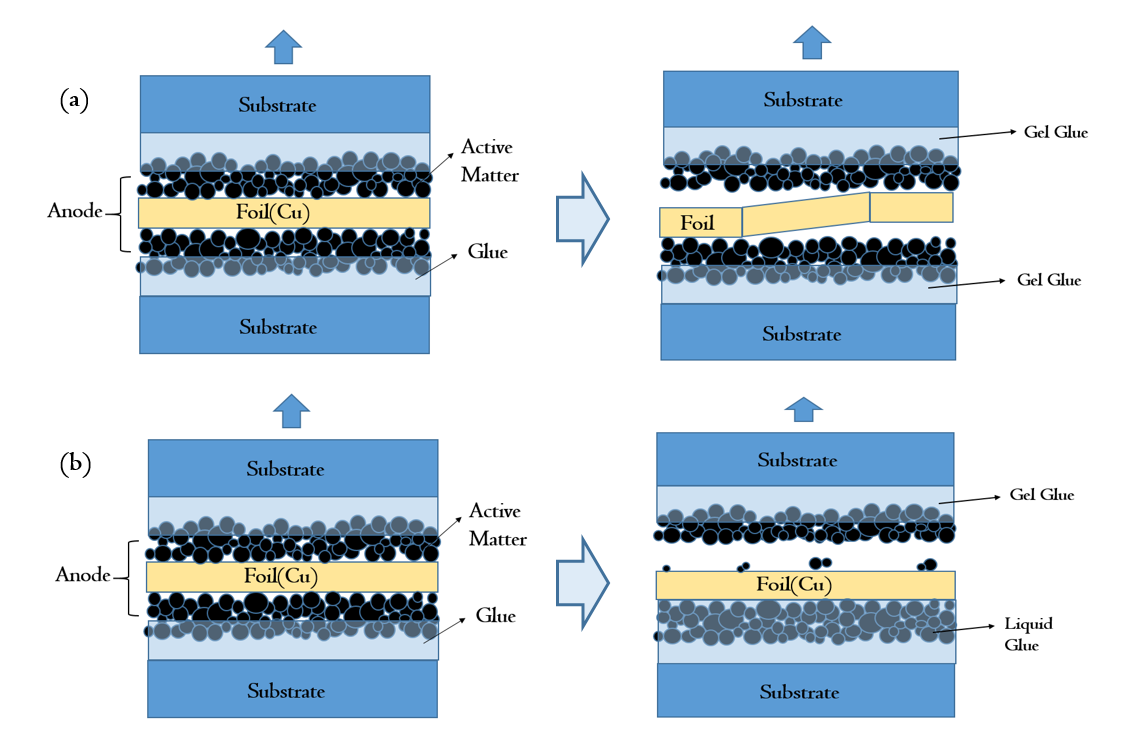
\includegraphics[width=\textwidth]{Geltype.png}
\caption{选用不同的胶水:(a)两侧选用凝胶使得可能发生图示失效 (b)一侧选用粘接性很强的液体胶从而使得只在凝胶侧发生失效} 
\label{fig:geltype}
\end{figure}
\subsubsection{混合拉伸-剪切实验设计}
\begin{figure}
\centering   
\includegraphics[width=\textwidth]{Combine.png}
\caption{混合拉伸-剪切实验设计:(a) 夹具和样品实物图 (b)混合测试示意图} 
\label{fig:combine}
\end{figure}
为了实现对于混合拉伸-剪切应力加载条件下的测试,设计了如图所示的实验夹具,如(b)所示,样品被粘接在两个基底上然后在固定在夹具上进行测试,夹具的加载方向实现了从$0^{\circ}$到$90^{\circ}$每隔$15^{\circ}$的一共七组加载条件的测试。 显然随着角度的增加,剪切分量增加。 静态实验的测试设备如图\ref{fig:equipment}所示,采用的静态测试速度为$1.0mm \times min^{-1}$,每个实验至少重复三次。 动态实验的测试则如图\ref{fig:dynamic}所示,可以实现中低速的动态加载和力学测试。
\begin{figure}
\centering   
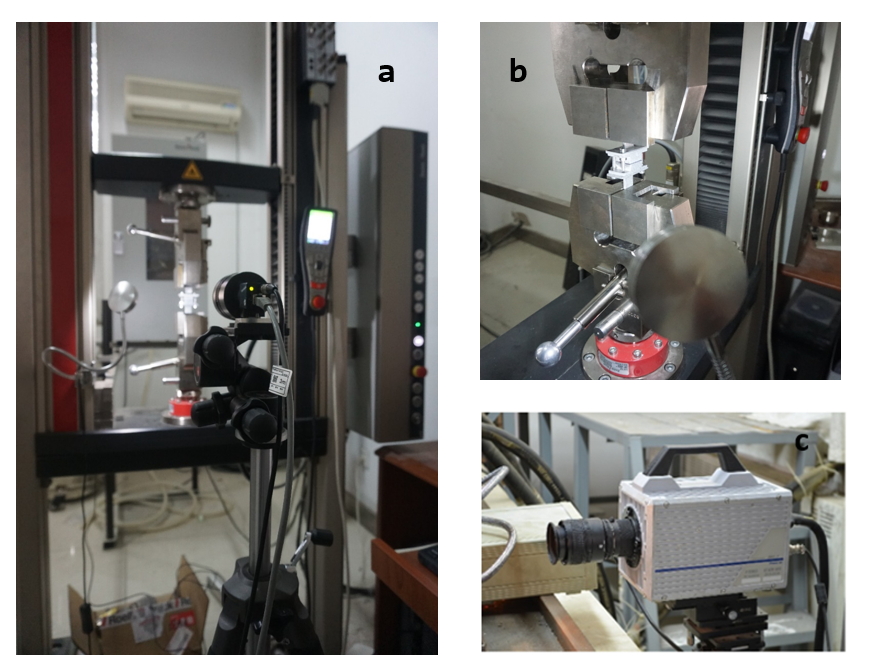
\includegraphics[width=\textwidth]{equip.png}
\caption{静态测试设备:(a)Zwick Z020 universal mechanical tester
(b) Tester with specimen (c)Digital image correlation(DIC) camera} 
\label{fig:equipment}
\end{figure}
\begin{figure}
\centering   
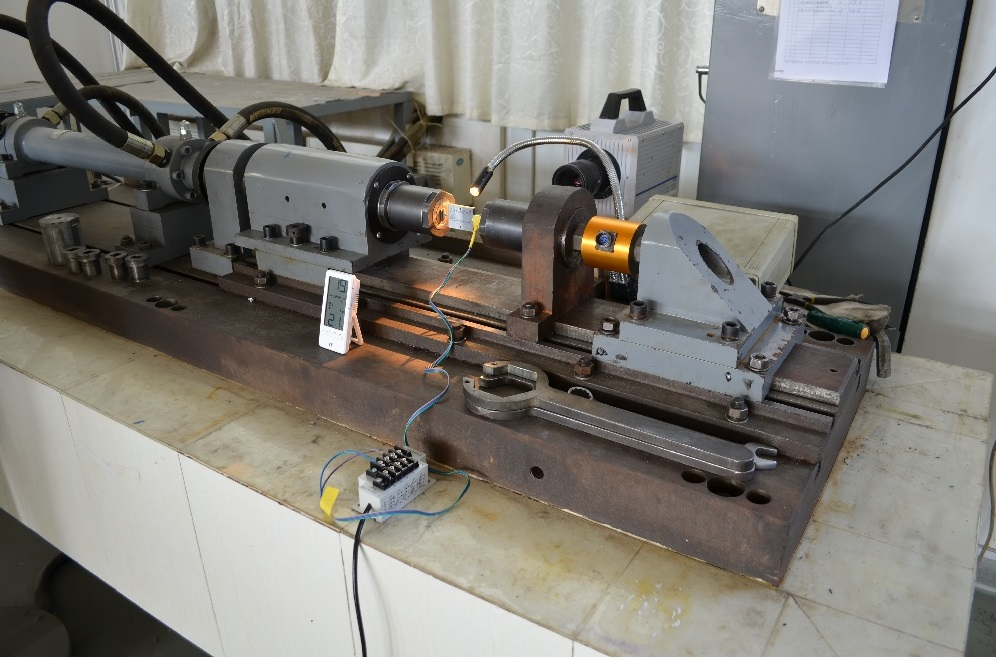
\includegraphics[width=\textwidth]{dynamic.png}
\caption{动态测试设备:液压加载水平台} 
\label{fig:dynamic}
\end{figure}
\section{实验准备和模型分析}
\subsection{测试样品分析:能谱测试}
正如之前所提到,实验成功的关键在于实现只在一侧发生活性层-集流体的脱层失效,之前的设计已经可以从原理上保证这一失效行为,但是还需要保证在发生断裂的这一侧,所涂布的凝胶不会有很强的渗透从而不会在断裂面上有凝胶的存在,从而不会对界面强度测试的结果产生影响。 基于此,对涂布的样品进行了沿着纵切面的电子能谱(Energy Dispersive Spectrdmeter,EDS)测试,其原理为,由于电极活性层中不含有硅元素,而所使用的特种凝胶中含有硅元素,所以通过测定硅元素在纵切面沿着深度的分布得到凝胶的渗透情况,测试结果如图\ref{fig:eds}所示。从图中可以看出,硅元素的分布只在很浅的表层,从而凝胶的渗透只在很浅的深度,不会影响到发生在活性层和集流体之间的断裂失效。
\begin{figure}
\centering   
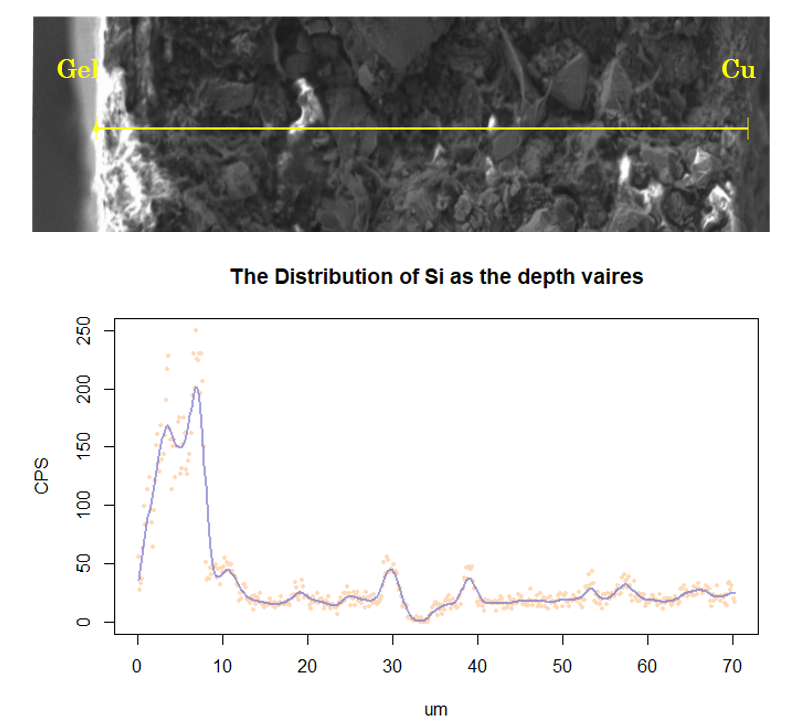
\includegraphics[width=\textwidth]{EDS.png}
\caption{沿着深度方向从涂胶侧到集流体侧的硅元素丰度的分布} 
\label{fig:eds}
\end{figure}
\subsection{断裂准则}
在本文所进行的活性层-集流体断裂失效行为的研究中,其中最为关键的是得到力学加载时的峰值力,也就是断裂失效对应的断裂强度。 之所以研究不同方向的加载以产生混合拉伸-剪切的实验加载条件,是为了准确表征界面断裂失效行为,从而对其进行表征从而预测其在各种混合工况下的失效行为。对于材料的断裂失效进行研究,最核心的便是研究清楚其屈服面以及对应可以采用的屈服准则,所以有必要首先对于材料的屈服特性乃至主要的屈服准则进行一个概要的介绍。
\subsubsection{屈服面}
通常而言,材料的屈服面是一个五维平面(六维应力空间中),其通常为凸集且在屈服面内材料处于弹性状态。 之所以叫做屈服面,也就是当材料的应力状态到达屈服面上一点(也就是其屈服点),材料就进入了塑性状态,并且进一步的加载只是会使得材料继续在该屈服面上移动,改变其应力状态\cite{Hughes}。\\
\indent 依据这样的假定,有许多针对具体材料特性和基于实验观测的屈服准则被提出。 
一般而言,屈服准则都被表达为三个主应力($\sigma_1,\sigma_2,\sigma_3$)或者应力的三个不变量($\mathbf{I_1},\mathbf{J_2},\mathbf{J_3}$)的函数形式\cite{Hughes}:
\begin{equation}
\mathnormal{f}(\sigma_1,\sigma_2,\sigma_3) = 0
\end{equation}
或者
\begin{equation}
\mathnormal{f}(\mathbf{I_1},\mathbf{J_2},\mathbf{J_3}) = 0
\end{equation}
需要指出的是,对于三个主应力,可以得出应力的三个不变量和它们的关系:
\begin{equation}
I_1 = \mathrm{Tr}(\mathbf{\sigma}) = \sigma_1 + \sigma_2 + \sigma_3
\end{equation}
\begin{equation}
J_2 = \frac{1}{2} \mathbf{s} : \mathbf{s} = \frac{1}{6} \left[(\sigma_1-\sigma_2)^2 + (\sigma_2-\sigma_3)^2 + (\sigma_3-\sigma_1)^2 \right]
\end{equation}
\begin{equation}
J_3 =det(\mathbf{s}) = \frac{1}{3}(\mathbf{s} \times \mathbf{s}) : \mathbf{s} =s_1s_2s_3
\end{equation}
其中,
\begin{equation}
s = \sigma - \frac{I_1}{3}\mathbf{I} 
\end{equation}
\subsubsection{主要屈服准则}
\begin{figure}
\centering   
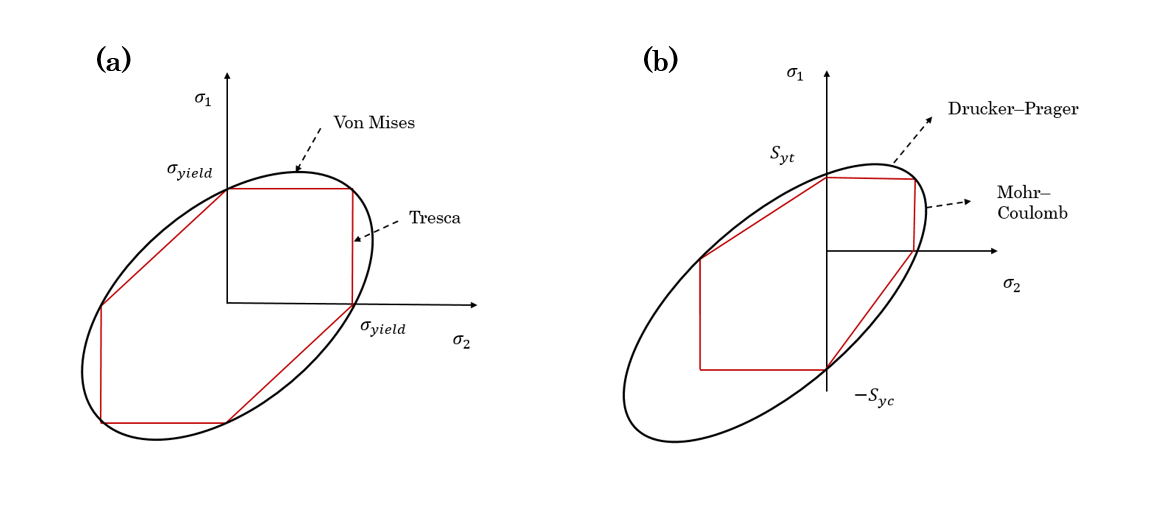
\includegraphics[width=\textwidth]{yield.png}
\caption{(a)Von Mises和Tresca失效准则 (b)Drucker-Prager和Mohr-Coulomb失效准则} 
\label{fig:yield}
\end{figure}
工程中常用的屈服准则有一下几种\cite{Jagab2005Theory}:
\begin{itemize}
	\item Tresca 失效准则\\
	Tresca失效准则又称最大切应力准则(Maximum shear stress theory),其数学表达为:
	\begin{equation}
	\frac{1}{2}\left(|\sigma_1-\sigma_2|,|\sigma_2-\sigma_3|,|\sigma_3-\sigma_1|\right)=S_{sy}=\frac{1}{2}S_y
	\end{equation}
	其中,$S_{sy}$是剪切失效强度而$S_y$是拉伸失效强度。主应力空间中Tresa屈服面是一个六边的菱形,其在受到静水压力(三个主应力大致相等)时材料一直保持弹性,而当主应力有不一致时,材料会受到剪切,若剪切到达屈服水平材料进入塑性。图\ref{fig:yield}(a)展示了二维应力空间的屈服面。
	\item von Mises 失效准则\\
	von Mises失效准则的数学表达为:
	\begin{equation}
	(\sigma_1 - \sigma_2)^2 + (\sigma_2 -\sigma_3)^2 + (\sigma_3-\sigma_1)^2 = 2S^2_y
	\end{equation}
	其中,$S_y$是拉伸失效强度。其失效面是一个圆柱体,轴向和三个主应力方向夹角相同,其在二维应力空间的屈服面呈现椭圆形,如图\ref{fig:yield}(a)所示。
	\item Mohr–Coulomb 失效准则\\
	Mohr-Coulomb准则和Tresca失效准则相似,只是考虑了材料的拉伸和压缩模量不同的情况,所以通常在表征土壤、混凝土等颗粒状材料的断裂中有很广泛的应用。其数学表达式为:
	\begin{multline}
	\frac{m+1}{2} \mathbf{max} \Big(|\sigma_1 - \sigma_2| + K(\sigma_1+\sigma_2),|\sigma_1 - \sigma_3| + K(\sigma_1+\sigma_3),|\sigma_2 - \sigma_3| + \\
	K(\sigma_2+\sigma_3)\Big) = S_{yc}
	\end{multline}  
	其中
	\begin{equation}
	m = \frac{S_{yc}}{S_{yt}}
 \quad K=\frac{m-1}{m+1}
 	\end{equation}
 	参数$S_{yc}$和$S_{yt}$分别是材料的压缩和拉伸失效强度,显然当材料的拉伸和压缩参数相同,即$S_{yc}=S_{yt}$时,该准则就会退化为Tresca准则。
 	图\ref{fig:yield}(b)展示了其在二维应力空间中的失效面。
	\item Drucker–Prager 失效准则\\
	和von Mises失效准则类似,该准则用于处理拉伸和剪切都可能引起断裂失效的情况,如对混凝土材料,其数学表达式如下:
	\begin{multline}
	\left(\frac{m-1}{2}\right)(\sigma_1 + \sigma_2 + \sigma_3 )+\left(\frac{m+1}{2}\right)
	\sqrt{\frac{(\sigma_1-\sigma_2)^2+(\sigma_2-\sigma_3)^2+(\sigma_3-\sigma_1)^2}{2}}\\
	=S_{yc}
	\end{multline}  
	其中
	\begin{equation}
	m = \frac{S_{yc}}{S_{yt}}
	\end{equation}
	其在二维应力空间的图线如图\ref{fig:yield}(b)所示。
\end{itemize}

\subsection{胶粘失效模型——内聚力模型}
对于大多数的断裂问题,诸如已经存在裂纹和裂纹前的应力奇异区域可以忽略的情况,应用线弹性断裂力学的工具就可以分析得到足够好的结果。但是对于韧性较大的材料和或者
粉体类材料,由于其塑性行为和微裂纹的影响,其发生断裂时裂纹尖端的非线性区不能被忽略。 而在这些情况下,由 Hillerborg 所提出的内聚力模型\cite{Hillerborg2008Analysis},便成为解决这些问题的重要工具。\\
\indent 特别地,对于复合材料而言,多种材料之间的脱层失效是诸如纤维增强材料断裂失效的主要模式。 脱层失效还可以在多种情形下发生,即使在低速甚至静态的外载,在结构点的受力都有可能引起脱层失效\cite{Elices2002The}。 由于脱层失效实际上很难被发现,所以对于其模式的研究和表征就显得十分重要。 对于这样的问题,内聚力模型提供了十分重要的工具。\\
\indent界面的脱层失效的断裂问题归根结底是不连续性的问题。 考察包含不连续(发生了断裂或者脱层)的区域$\Omega$,而$\Gamma_d$将区域$\Omega$划分为两部分,$\Omega_{+}$和$\Omega_{-}$。而在边界$\Gamma_{F}$上有预先给定的外力。 则可以用一下方程描述区域内的应力$\sigma_{ij}$(用$\sigma^{+}_j$和$\sigma^{-}_j$表示不连续的应力)\cite{Turon2007An}:
\begin{equation}
\sigma_{ij,j} = 0 \quad in \quad \Omega
\end{equation}
\begin{equation}
\sigma_{ij}n_j = t_i  \quad on \quad \Gamma_F
\end{equation}
\begin{equation}
\sigma_{ij} n^{+}_j = \tau^{+}-i = -\tau^{-}_i = \sigma_{ij}n^{-}_j \quad on \quad \Gamma_d
\end{equation}
\indent 内聚力模型假定在断裂区产生一个粘接损伤带(Cohesive damage zone),从而可以将微结构的失效和连续力学场建立联系。 后文将利用这一模型的一个引申结论表征不同角度加载活性层的断裂失效强度。 \\
\indent 内聚力模型相比经典的断裂力学(线弹性断裂力学,裂纹尖端张开位移法)有着下列主要的优点:
\begin{itemize}
	\item 可以相对准确地预测材料的断裂失效
	\item 在分析中非线性区域不需要被忽略
\end{itemize}
实际上,内聚力模型本身并不基于任何材料模型,其本质上只是对材料之间被拉开时对于其间的粘接力的一个描述。 当粘性表面发生分离时,牵引力增加,直到达到最大值,然后随后减小到零,最终导致完全分离。 将牵引力-位移曲线绘制出便得到了牵引-位移曲线,同时该曲线下和坐标轴所围成的面积和分离所消耗的能量相等。 可以看出内聚力模型保持着连续性条件,在实现了物理上的分离的同时消除了应力的奇异度。更具体而言,内聚力模型所给出的牵引-位移曲线相当于给定了材料的断裂本构。\\
\indent 首先本文给出了内聚力模型的示意图\ref{fig:crack}(a)和其经典的牵引-分离曲线\ref{fig:crack}(b)。
\begin{figure}
\centering   
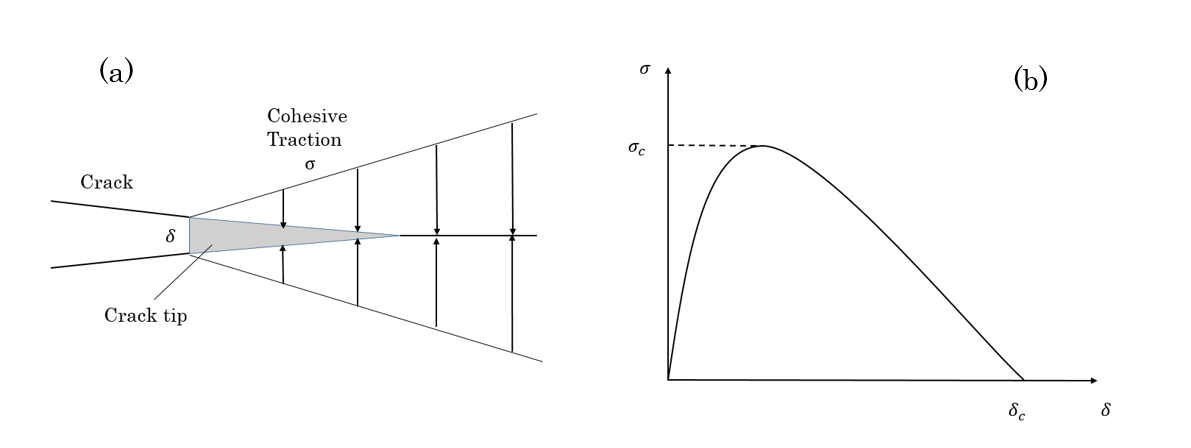
\includegraphics[width=\textwidth]{crack.png}
\caption{(a)内聚力模型示意图 (b)典型的牵引-分离曲线} 
\label{fig:crack}
\end{figure}
一般地,可以用下式来描述内聚模型中的牵引-分离关系
\begin{equation}
\sigma = \sigma_c \mathnormal{f}(\delta / \delta_c)
\end{equation}
其中,$\delta_c$是分离力的峰值,而$\sigma_c$是分离的特征位移。其无量纲的分离函数$\mathnormal{f}$和失效机理相关。\\
同时也可以求出粘接能量密度,也就是分离单位面积所需要做的功:
\begin{equation}
\Gamma_c = \int^{\delta_c}_0 \sigma(\delta) d\delta
\end{equation}
也就是曲线和坐标轴所围成的面积。下面将介绍一些对于函数$\mathnormal{f}$的一定程度的简化求解方法\cite{Elices2002The}:
\begin{enumerate}
	\item Dugdale 模型\\
	对韧性材料而言,其带状塑性区就是粘性区域,而屈服应力就是牵引力,如图\ref{fig:czm}(a)所示:
	\begin{equation}
	\sigma = \sigma_c
	\end{equation}
	同时有
	\begin{equation}
	\Gamma_c = \sigma_c\delta_c
	\end{equation}
	在使用这一模型时,完全分离在$\delta = \delta_c$时发生。
	\item 线性软化模型\\
	这一模型通常被用于模拟诸如陶瓷和混凝土这样的准脆性材料。其牵引-分离准则如下:
	\begin{equation}
	\sigma = \sigma_c(1-\delta/\delta_c)
	\end{equation}
	同时有
	\begin{equation}
	\Gamma_c = \frac{1}{2} \sigma_c \delta_c
	\end{equation}
	如图\ref{fig:czm}(b)所示,牵引力首先达到最值$\sigma_c$,然后随着分离位移增加而减小,最终在分离点$\delta_c$等于零。
	\item 梯形模型
	显然梯形模型\ref{fig:czm}(c)可以看成是上面的线性软化模型的一种延伸,其牵引-分离关系如下:
	\begin{equation}
	\sigma = 
	\begin{cases}
	\sigma_c(\delta/\delta_1)&\text{$0 \leq 
	\delta \leq \delta_1$}\\
	\sigma_c&\text{$\delta_1 \leq \delta \leq \delta_2$}\\
	\sigma_c(\delta_c-\delta)(\delta_c-\delta_2)&\text{$\delta_2 \leq \delta \leq \delta_c$}
	\end{cases}
	\end{equation}
	同时有
	\begin{equation}
	\Gamma_c = \frac{1}{2} \sigma_c (\sigma_c + \sigma_2 - \sigma_1)
	\end{equation}
	\item 指数模型\\
	基于原子尺度的模拟\cite{Rose1981Universal},可以建立指数形式的模型\ref{fig:czm}(d):
	\begin{equation}
	\sigma = \sigma_c \left(\frac{\delta}{\delta_0}\right)exp\left(1-\frac{\delta}{\delta_0}\right)
	\end{equation}
	其中,$\delta_0$是达到峰值牵引力$\sigma_c$时的分离位移,同时可以给出能量的计算公式:
	\begin{equation}
	\Gamma_c = \int^{\infty}_0 \sigma d\delta = \mathnormal{e} \sigma_c \delta_0
	\end{equation}
\end{enumerate}
\begin{figure}
\centering   
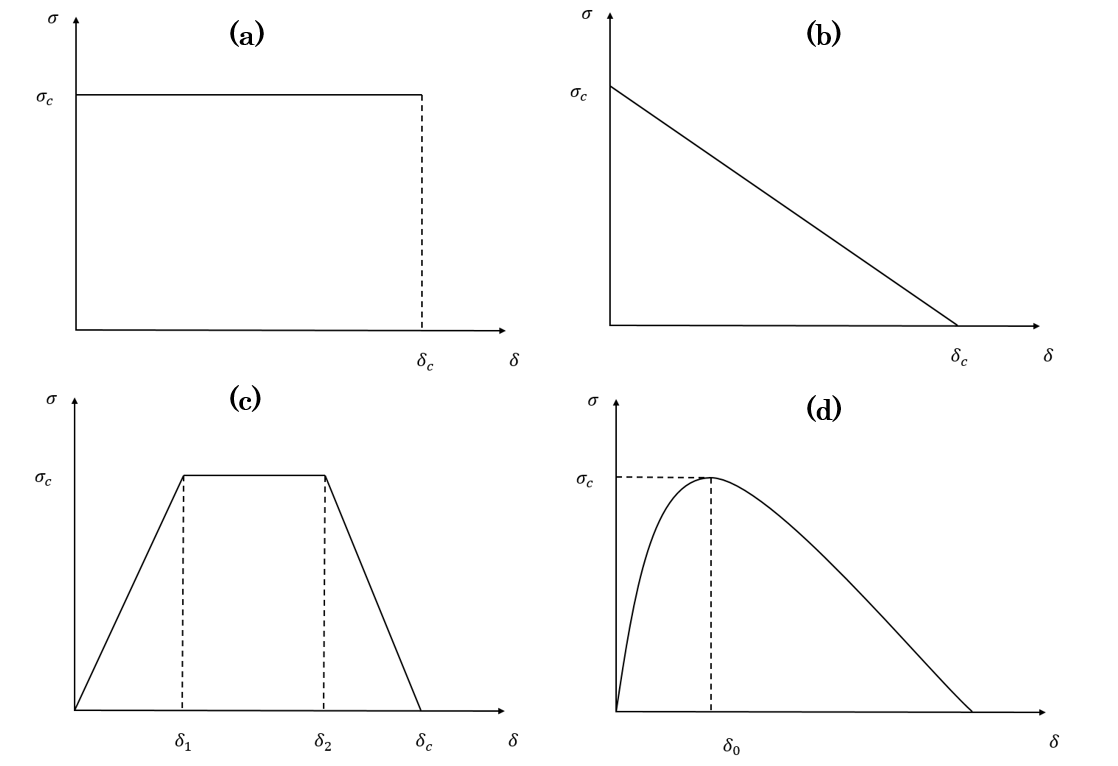
\includegraphics[width=\textwidth]{czm.png}
\caption{内聚力模型: (a)Dugdale 模型 (b) 线性软化模型 (c)梯形模型 (d)指数模型} 
\label{fig:czm}
\end{figure}

\chapter{实验结果和分析}
\section{静态实验}
\subsection{断裂模式分析}
\begin{figure}
\centering   
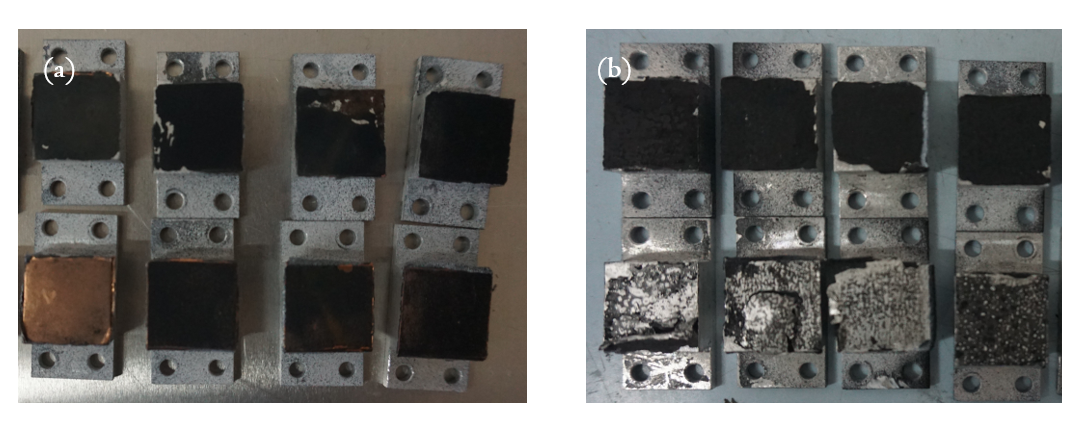
\includegraphics[width=\textwidth]{failure_ac.png}
\caption{正负极拉伸实验样品断裂图} 
\label{fig:ac}
\end{figure}
\begin{figure}
\centering   
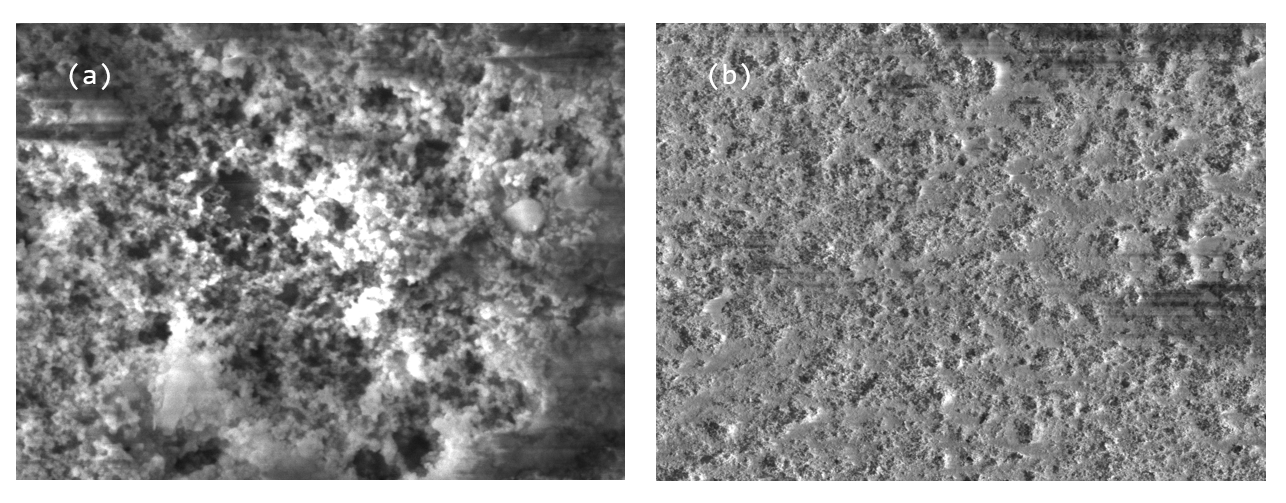
\includegraphics[width=\textwidth]{SEM.png}
\caption{样品断裂面的电镜照片:(a)活性物质侧 (b)金属箔侧} 
\label{fig:sem}
\end{figure}
按照第3章中所介绍的实验设计我们分别进行了电池正极和负极的从$0^{\circ}$到$90^{\circ}$的静态加载测试,实验中得到的正极和负极样品的断面如图\ref{fig:ac}所示。同时,也对实验后的断面进行了扫描电镜的检查,其结果如图\ref{fig:sem}所示。
可以看出,对于所有的样品都得到了所设定的在凝胶侧的集流体和活性层的脱层失效的断裂模态。 但是比较不同角度的加载测试,其测试结果却呈现出复杂的混合拉伸-剪切失效模态。 从$0^{\circ}$到$90^{\circ}$,失效模态发生了显著的变化。 对于$90^{\circ}$拉伸即单向拉伸测试,粘接失效是主要的失效模态,而在试验中可以观测到几乎所有的活性颗粒都会从集流体上脱落,而对于$0^{\circ}$拉伸测试即纯剪测试而言,活性层会有相当部分附着在集流体上只有一小部分集流体清晰可见。 可以看出前文所提到的失效模式中的Cohesion(即活性层内部的断裂失效)和Adhesion(活性层和集流体之间的脱层失效)两种失效模式在其中均发挥着作用。而考虑到之前所提到的活性层中粘结剂的法向分布\cite{M2017Investigation},在所有的加载角度,Adhesion失效模态应该都是主导的失效模式。如图\ref{fig:mech}所示,靠近底层的颗粒的胶层的厚度要比其他层要薄一些,虽然这样会得到最内层最为薄弱的结论,但是其实对于最内层而言,颗粒和集流体金属箔之前的接触面积可能会相对较大,从而对于剪切加载而言\ref{fig:mech}(b),颗粒和活性层之间的剪切强度可能对比垂直方向上颗粒之间的粘接强度要高,从而会造成在剪切实验中,断裂面的集流体一侧上依然会附着有不少的活性物质颗粒。 而随着加载角度的变化,剪切的成分增加,不同深度处的活性层颗粒之前可能会发生的相对滑移和挤压会使得剪切强度增加。 同时,需要指出的是,对于活性层-集流体粘接的界面,其剪切失效强度依然只由粘结剂和粘结剂对集流体和活性颗粒之间的粘接情况相关。
\begin{figure}
\centering   
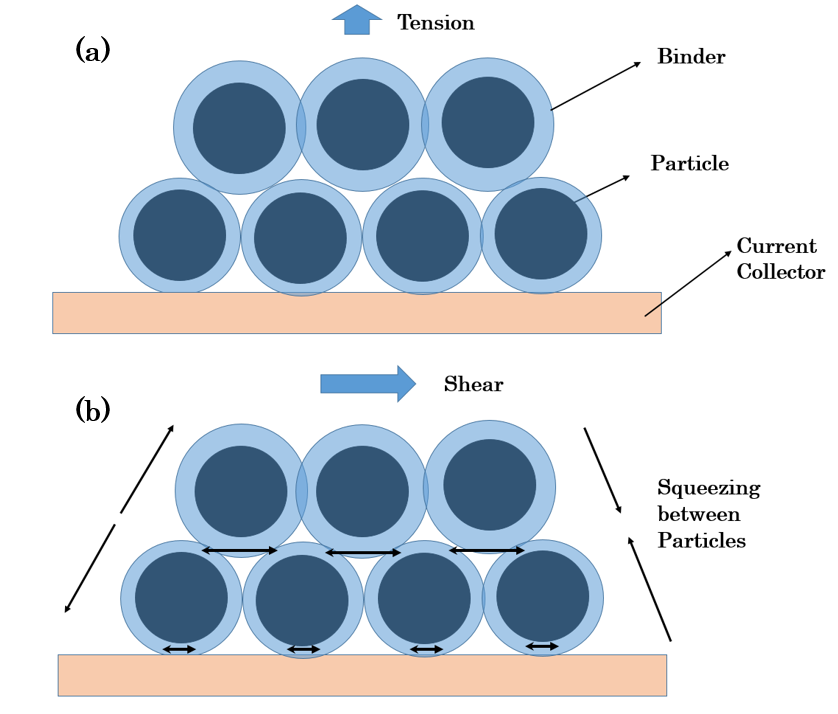
\includegraphics[width=\textwidth]{failure_me.png}
\caption{断裂失效的示意图:(a)拉伸 (b)剪切} 
\label{fig:mech}
\end{figure}
\subsection{不同应力状态下的粘接强度}
所有的实验样品其截面均为$20 \times 20(mm)$,假设应力在截面上均匀分布,则有效断裂强度可以用下式求得:
\begin{equation}
\sigma_{\mu} = F_f/A
\end{equation}
其中,$F_f$是力学加载过程中的峰值力,而$A$为断裂面的面积。电池正极和负极的测试结果分别如图\ref{fig:strength}(a)(b)所示。可以看出,正极和负极的结果呈现出不同的规律:
\begin{itemize}
	\item 对正极而言,断裂强度分布在1.0MPa到2.4MPa之间,从$0^{\circ}$到$60^{\circ}$,断裂强度整体呈现下降趋势,但在$45^{\circ}$处呈现出反常并取得其最大值,而在$75^{\circ}$处也出现了一个极值,可以看出在混合拉伸-剪切的加载下,有着相对较大的剪切分量加载下其粘接强度会有所提升
	\item 对负极而言,断裂强度分布在0.9MPa到2MPa之间,而主要集中分布在1.25MPa上下,只在$15^{\circ}$和$75^{\circ}$处有所反常分别出现了最大值和最小值,这可能是由于负极活性层相比正极而言涂布较薄,失效模态相对集中。
\end{itemize}
总之,电极的粘接强度的混合拉伸-剪切失效呈现出复杂的变化规律,而总体而言正极活性层的粘接强度要显著高于负极的粘接强度,这也和之前的对电池的挤压等测试的结果相一致\cite{Luo2017Mechanical}。
\begin{figure}
\centering   
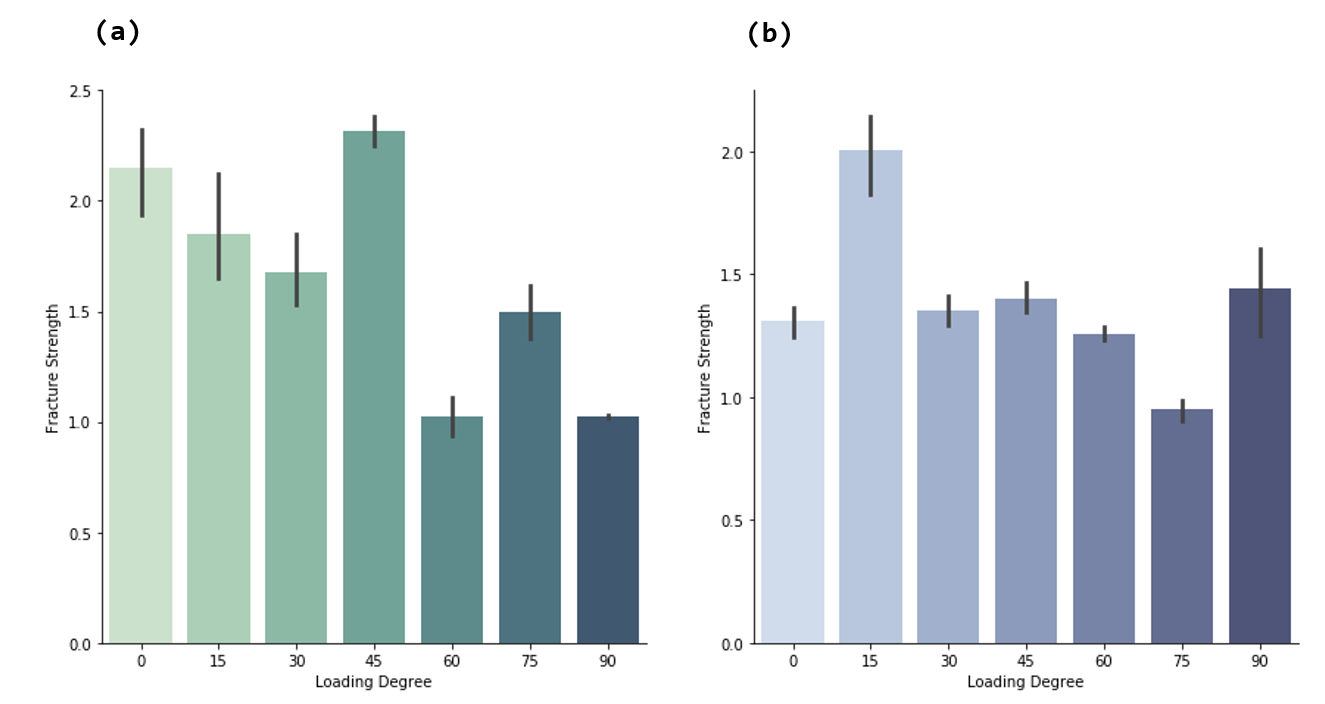
\includegraphics[width=\textwidth]{Strength.png}
\caption{不同角度的粘接强度测试结果:(a)正极 (b)负极} 
\label{fig:strength}
\end{figure}
\indent 对于这一实验,整体的断裂强度可以被分解为拉伸和剪切两个独立分量:
\begin{equation}
\sigma_n =\sigma_{\mu}sin\theta
\end{equation}
\begin{equation}
\sigma_s =\sigma_{\mu}cos\theta
\end{equation}
\begin{figure}
\centering   
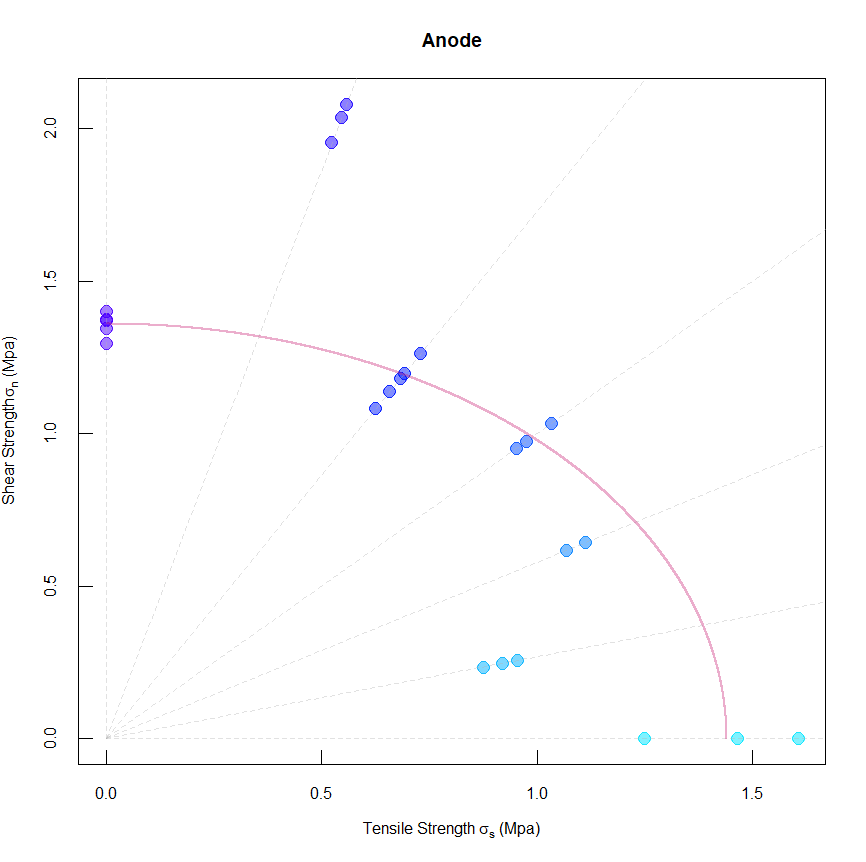
\includegraphics[width=\textwidth]{circle_a.png}
\caption{不同测试的拉伸和剪切分量:正极} 
\label{fig:circle_a}
\end{figure}
\begin{figure}
\centering   
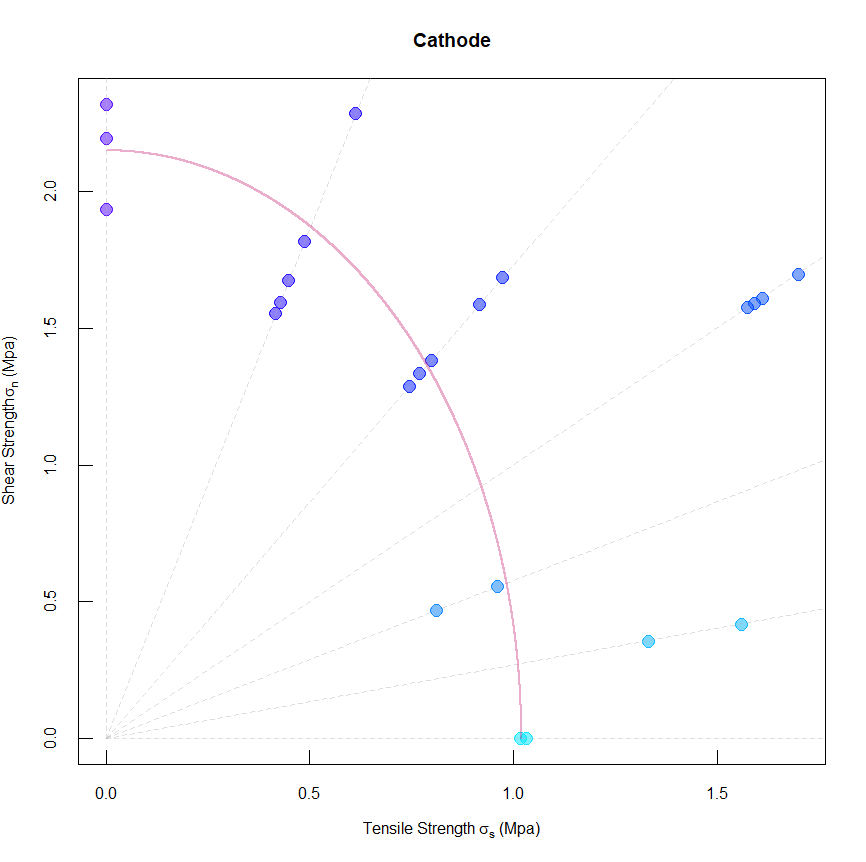
\includegraphics[width=\textwidth]{circle_c.png}
\caption{不同测试的拉伸和剪切分量:负极} 
\label{fig:circle_c}
\end{figure}
其中,$\theta$是加载角度,从$90^{\circ}$到$0^{\circ}$分别从单向拉伸变化到纯剪切加载,而$\sigma_n$和$\sigma_s$分别是拉伸和剪切分量。 可以在$\sigma_n - \sigma_s$平面分别画出结果\ref{fig:circle_a}和\ref{fig:circle_c},并可以采用之前所分析的内聚力模型(Cohesive zone model)来表征粘接失效行为:
\begin{equation}
\left(\frac{\sigma_n}{NFLS} \right)^2 + \left(\frac{\sigma_s}{SFLS} \right)^2 = 1
\end{equation}
两个椭圆线的拟合参数NFLS和SFLS分别为拉伸和剪切的失效应力。 在图\ref{fig:circle_a}\ref{fig:circle_c}中,对正极和负极分别进行拟合绘制出虚线所示的失效线。可以看出对于正极(NFLS = 1.42MPa, SFLS = 1.40MPa)而言,失效线低估了整体的失效行为,而对负极(NFLS = 1.36MPa, SFLS = 1.44MPa)则是相对高估(除去其中$15^{\circ}$的情形)。

\section{动态实验}
除了静态实验之外,对正极和负极还进行了$0.1m/s$和$1m/s$分为$90^{\circ}$,$60^{\circ}$和$30^{\circ}$的加载测试,不同速度下的测试结果如图\ref{fig:a}和\ref{fig:c}所示(动态测试时较高速度下正极铝箔出现明显断裂故没有采用正极的$1m/s$的实验数据)。可以看出,在应变率增加时(随着加载速度增加),界面断裂强度均有显著提升,但是在动态加载的不同速度即$0.1m/s$和$1m/s$加载结果的比对中,断裂强度没有体现出明显的应变率效应。 而且随着加载角度的变化,剪切分量的增加,在不同加载速度下的断裂强度有着不同的变化趋势。 对于正极和负极而言,在较为低速的加载即$0.1m/s$的加载下(图\ref{fig:a}和\ref{fig:c}中绿色条形),随着剪切分量的增加,断裂强度呈现先增加后减小的趋势;而在较高速度的加载即$1m/s$的加载下,断裂强度却呈现和之前不同的出先下降后上升的变化趋势(见图\ref{fig:a}红色条形)。
\begin{figure}
\centering   
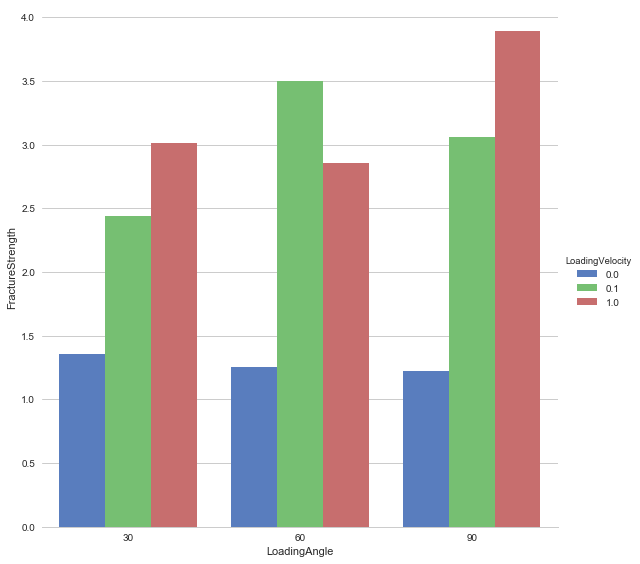
\includegraphics[width=\textwidth]{a.png}
\caption{不同加载速度下的不同角度的断裂强度试验结果:负极} 
\label{fig:a}
\end{figure}
\begin{figure}
\centering   
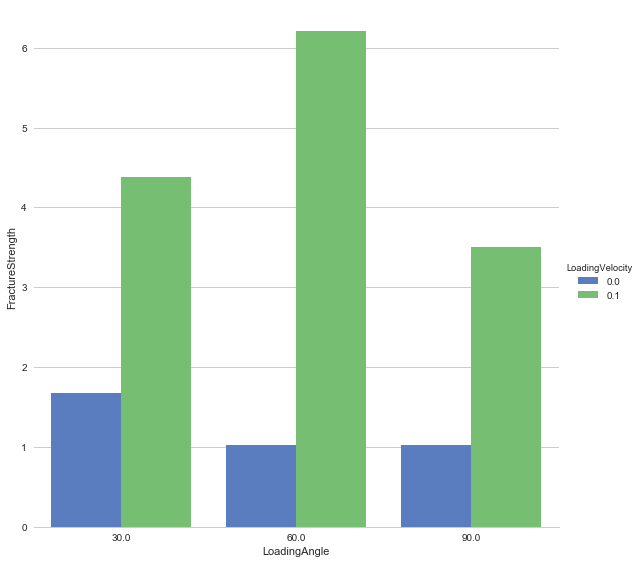
\includegraphics[width=\textwidth]{c.png}
\caption{不同加载速度下的不同角度的断裂强度试验结果:正极} 
\label{fig:c}
\end{figure}

\section{模型建立:力学-化学耦合模型}
在本文的研究中,对于集流体和活性层的宏观测试,无论从实验的断裂面还是从实验测得的实际的断裂强度而言,都表明在电极材料的脱层失效中,颗粒-粘结剂-集流体界面才是最容易发生断裂失效的位置;另一方面,扩散过程中会引起整个活性颗粒乃至胶接表面的应力的重新分布,这是需要在理论和实验研究中需要考虑的关键因素。基于这两点,可以引出对于电池中活性颗粒粘结剂界面力学特性研究的颗粒-壳体模型,其可以综合考量力学和化学因素对于界面力学特性的影响,本文对这一模型在总结中进行介绍和分析,以期能在这一基础上结合本文的研究,进而考虑更加充分的因素改进和修正模型,进行进一步的电池建模研究。
\begin{figure}
\centering   
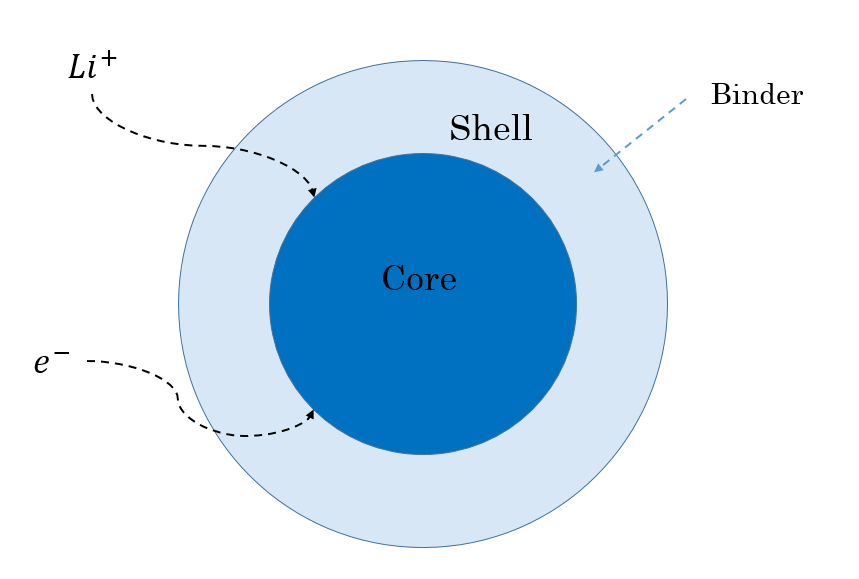
\includegraphics[width=\textwidth]{coreshell.png}
\caption{颗粒-壳体模型示意图。颗粒被粘结剂均匀的包裹,形成外层的壳体,而电子和锂离子在壳体和粘结剂的界面处发生反应,锂离子会进一步向着颗粒内部扩散} 
\label{fig:cs}
\end{figure}
\\
\indent 如图\ref{fig:cs}所示,这一颗粒-壳体模型实际上是由包裹着粘结剂的球形活性颗粒两部分构成。在介绍模型的控制方程之前,需要给定模型的基本假设\cite{Takahashi2016Mechanical}:
\begin{enumerate}
	\item 模型假设活性颗粒之间的相互作用可以忽略并且颗粒之间的电流分布是均匀的。 前一个假设可以由电极活性层的孔隙率保证,而后一个要求电极颗粒的尺寸分布比较均匀和电极的涂布厚度在电极颗粒的尺度误差不大,这些条件在现有的电极生产工艺中可以得到保证\cite{Takahashi2015Examination}。
	\item 不考虑SEI(solid electrolyte interface)膜,即固体电解质界面膜的影响。这一点也被之前对于有着SEI膜影响的活性层的力学性质的实验测定\cite{Zhang2012Direct}和数值模拟\cite{Zheng20143D}所佐证,其影响相对于粘结剂而言可以忽略。
	\item 为了定义边界条件的方便,假定活性颗粒的半径和胶层的厚度在锂离子的脱嵌和嵌入过程中保持不变。 实质上而言,这是一个很强的假设,但是这一假设依然可以给出相当准确的力学分析,因为体积的变化的绝对值还是很小。 但是需要指出的是,进一步的对于硅电极和锡电极的研究中,必须要考虑由于锂离子输运造成的体积变化对于边界条件的影响。
\end{enumerate}
接下来介绍模型的核心理论部分。首先,依据之间的研究\cite{Zhang2007Numerical},给出锂离子在柱坐标中的扩散方程:
\begin{equation}
\label{eq:ch}
\frac{\partial c}{\partial t} = D_s \left( \nabla^2 c -\frac{\Omega}{RT}\nabla c \nabla \sigma_h -\frac{\Omega_c}{RT}\nabla^2 \sigma_h \right)
\end{equation}
其中,$c$是离子密度,$D_s$是扩散系数,$R$是气体常数,$T$是开尔文温度,$\Omega$是锂离子的偏摩尔体积(一定量溶质溶在一摩尔溶液中所引起的体积变化),$\sigma_h$为静水压力。\\
对于力学量,由方程\ref{eq:list1},\ref{eq:list2}和\ref{eq:list3}描述:\\
\begin{align}
\label{eq:list1}
\frac{d \sigma_r}{d r} &+\frac{2}{2}(\sigma_r - \sigma_t)  = 0\\
\label{eq:list2}
\sigma_r =& \frac{E}{(1+\nu)(1-2\nu)} \left[(1-\nu)\frac{d \mu}{d r} +2\nu \frac{\mu}{r} - (1+\nu)\frac{\Delta c \times \Omega}{3} \right] \\
\label{eq:list3}
\sigma_t =& \frac{E}{(1+\nu)(1-2\nu)} \left[\nu\frac{d \mu}{d r} + \frac{\mu}{r} - (1+\nu)\frac{\Delta c \times \Omega}{3} \right]
\end{align}
其中,$\sigma_r$是径向应力分量,$\sigma_t$是切向应力分量,$E$是杨氏模量,$\nu$是泊松比,$\mu$是位移向量,$\Delta c = c-c_0$。\\
方程\ref{eq:ch}为偏微分方程,求解需要给出初始和边界条件:
\begin{align}
c_0=0 \quad & at \quad t=0\\
-D_s\left(\nabla c - \frac{\Omega c}{RT} \nabla \sigma_h \right) = 0 \quad & at \quad r=0\\
-D_s\left(\nabla c - \frac{\Omega c}{RT} \nabla \sigma_h \right) = \frac{i_n}{F} \quad & at \quad r=r_0
\end{align}
同时还有一个自然边界条件:
\begin{equation}
\mu = 0 \quad at \quad r=0
\end{equation}
将颗粒内和胶层内的应力分布联系起来的条件是径向应力在界面处($r=r_0$)的连续性。\\
\indent 接下来,和颗粒内部类似,给出胶层内部的应力分布的控制方程:
\begin{align}
\label{eq:glue1}
\frac{d \sigma_r}{d r} &+ \frac{2}{r}(\sigma_r - \sigma_t) = 0\\
\label{eq:glue2}
\sigma_r =& \frac{E}{(1+\nu)(1-2\nu)}\left[(1-\nu)\frac{d \mu}{d r} + 2\nu \frac{\mu}{r} \right]\\
\label{eq:glue3}
\sigma_t =& \frac{E}{1+\nu}{1-2\nu}\left( \nu\frac{d \mu}{d r}+\frac{u}{r} \right)
\end{align}
值得注意的是,方程\ref{eq:list2}和方程\ref{eq:list3}中的描述锂离子嵌入和脱嵌的第三项没有在方程\ref{eq:glue2}和方程\ref{eq:glue3}中出现。\\
最后给出胶层表面的边界条件:
\begin{equation}
\sigma_r = 0 \quad at \quad r = r_0 + L 
\end{equation}
其中,L是胶层的厚度,这一边界条件实际上说明了没有外力作用。\\
\indent 
依据以上的模型,以求对于界面力学失效行为的微观本质进行模型构建和分析,有着十分重要的意义,接下来我们还将对于前文所没有关注的电化学行为对于电极活性层在颗粒层面的力学特性的影响进行分子模拟的研究,从而从另外一个角度对于这一模型进行完善和补充。
\section{总结和结论}
本章应用设计的混合拉伸-剪切实验方法对于电池正极和负极的活性层-集流体界面胶接强度进行了多种力学加载状况下的测试,并实施了不同速度加载下的动态实验。本章所得到的主要结果如下:
\begin{itemize}
	\item 在拉伸-剪切混合加载实验中,集流体-活性层界面的断裂失效模式会随着剪切分量的变化而发生变化。 其中,在拉伸测试中,主要发生粘接失效,即可以观测到几乎所有的活性层颗粒都会从集流体上脱落。 而在剪切测试中,活性层大多发生相对靠内部的断裂失效,即会有相当一部分活性颗粒继续粘接在集流体上,只有一部分集流体清晰可见。
	\item 在静态多角度加载实验中
	\begin{itemize}
		\item 对正极而言,断裂强度呈现从$1.0MPa$到$2.4MPa$的分布,随着剪切分量的减小(即加载角度从$90^{\circ}$逐渐减小),断裂强度逐渐下降,但是在中间角度如$45^{\circ}$处出现反常取得最值。 总体而言,在较大的剪切分量加载下粘接强度会有所提升。
		\item 对负极而言, 断裂强度要相对小于正极的断裂强度,其分布在$0.9MPa$到$2MPa$之间,并且在$1.25MPa$上下有着明显的集中,推测是由于负极活性层的涂布厚度相对较薄,从而失效模态对应的断裂强度也会比较集中。
	\end{itemize}
	\item 进行的$0.1m/s$和$1m/s$的加载实验表明,动态加载下界面的断裂强度有着显著的提升。 以$0.1m/s$加载为例,对于正极和负极,其不同加载角度下的断裂强度均有着高于两倍的提升。 同时,基于在不同速度加载的比较可以看出其断裂强度随着应变率的变化有着较低的阈值,在加载速度高于一定值($0.1m/s$)后,应变率变化引起的断裂强度的改变不是很明显。 此外,在不同加载速度下,断裂强度随着加载角度的变化也呈现了不同的变化规律。在$0.1m/s$加载速度下,断裂强度呈现先增加后减小的趋势,而在$1m/s$的加载下断裂强度变化呈现相反的趋势。
\end{itemize}


\chapter{分子模拟——锂离子迁移过程中弹性常数计算及断裂行为模拟}
\section{研究背景}
锂离子电池的电极材料在锂离子的扩散过程,即电池的充放电循环中,其活性颗粒会有相当大的体积变化,以常见的负极材料石墨为例,其体积在锂离子的嵌入过程中会增加大约10\% \cite{Dahn1991Phase},而在锂离子的容纳量上超出石墨十倍的硅则在嵌入锂过程中会有高达300\% 的体积增长\cite{Beaulieu2003The}。
\begin{figure}
\centering   
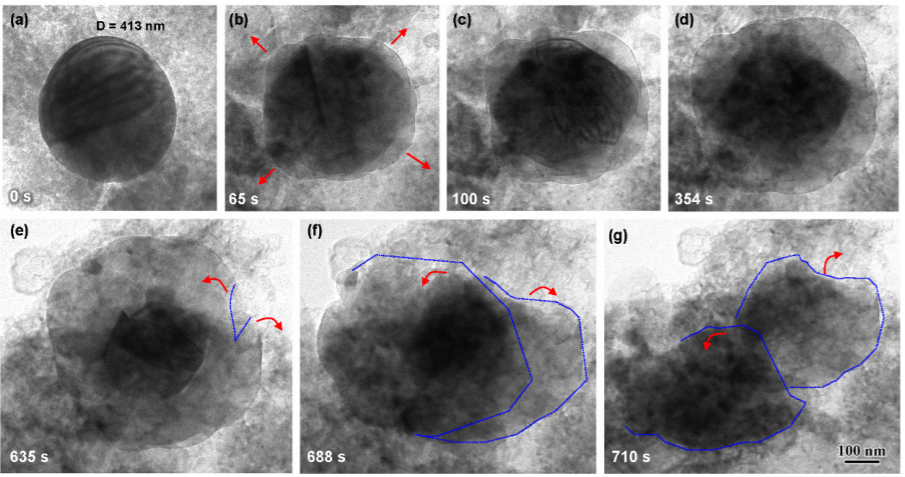
\includegraphics[width=0.8\textwidth]{Si.png}
\caption{硅颗粒在充放电过程中的开裂\cite{Beaulieu2003The}} 
\label{fig:Si}
\end{figure}
就微观层面上而言,锂离子电池的活性颗粒内部的力学强度在维持锂离子电池电极的力学完整性上有着重要的作用\cite{Lee2014Molecular}。由此可见,由于锂离子扩散(Li diffusion-induced stress, DIS)引起的应力是造成体积变化乃至电极断裂的重要因素。同时,由于应力产生和锂离子扩散过程的相互作用,使得这一问题涉及了力学、电化学乃至热力学多个方面物理因素的耦合。\\
\indent 近些年来,很多研究者希望通过调控DIS来增强锂离子电池的力学强度和耐久性\cite{Christensen2005A,Christensen2006Stress,Zhang2007Numerical,Verbrugge2009Stress,Cheng2008The,Zhang2008Intercalation}。如,Wolfenstine等人建立了基于杨氏模量、断裂强度乃至体积变化的对于颗粒尺寸影响容量消退的模型\cite{Woodford2010},Zhao等人则基于断裂力学和扩散动力学发展了判断钴酸锂颗粒断裂失效的准则\cite{Zhao2010Fracture}。 但是,这些研究的模型,多数只考虑体积变化造成的应力,从而不能真实反映实际复杂的电极材料的断裂失效行为。另外,这些模型都是基于固体扩散理论和连续介质力学的方程,需要一系列的诸如弹性常数(如弹性张量的分量,体材料的剪切和杨氏模量),表面能,扩散系数和体积膨胀率。 其中,模型中对于杨氏模量等力学参数的选取并未考虑其随着锂离子扩散的变化而给定为常值,这其实是因为处理不同SOC的电极材料进行力学特性的测试十分困难(由于锂离子和氧气的高度反应活性和制备大晶体的困难),从而应用数值模拟的手段得到这些参数和参数的动态变化就显得十分重要。\\
\indent如图\ref{fig:LiBattery}所示,在充放电过程中$LiFePO_4$电池会发生电极反应:
\begin{equation}
\label{eq:anode}
Anode : \quad Li_xC_6 -x e^{-} \to x Li^{+} +C_6
\end{equation}
\begin{equation}
\label{eq:cathode}
Cathode : \quad Li_{1-x}FePO_4 +x e^{-} + x Li^{+} \to LiFePO_4
\end{equation}
\indent 在充电时,外电压驱动锂离子从$LiFePO_4$晶体中脱出经过电解液到达石墨层,放电时则相反。显然,周期性的脱嵌和嵌入使得电极的正极和负极材料都会经历周期性的体积变化和诱导应力的产生,从而有可能造成电极材料的断裂失效进一步引起电池容量减小,这也是本章模拟需要揭示和研究的核心问题。

\begin{figure}
\centering   
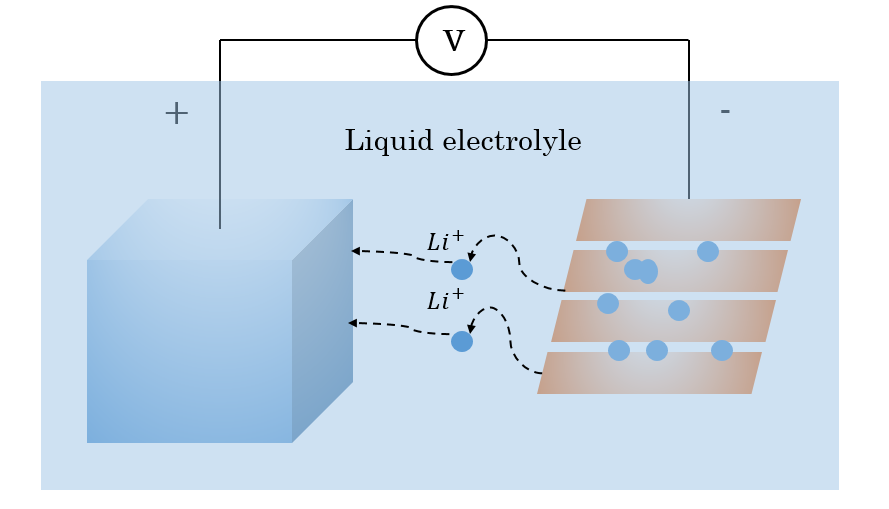
\includegraphics[width=0.8\textwidth]{LiBattery.png}
\caption{锂离子电池电化学通路示意图\cite{Tarascon2001Issues}} 
\label{fig:LiBattery}
\end{figure}
\section{锂离子在磷酸亚铁锂晶体中的迁移过程及其弹性常数:密度泛函矩阵方法}
\subsection{简介:磷酸铁锂材料}
磷酸铁锂作为锂离子电池的电极材料其理论的容量为170mAh/g,其嵌锂电位为3.5V, 并有着很良好的热稳定性。 另外,磷酸铁锂由于其低廉的价格和相对的低污染成为了很多商用锂离子电池电极材料的选择。室温下,磷酸铁锂通过在磷酸铁和磷酸铁锂间的相变转换来进行充放电循环,其反应方程见方程\ref{eq:anode}和方程\ref{eq:cathode}。\\
\indent 磷酸铁锂属于正交晶系,其晶格常数为a = 10.3375 $\dot{A}$, b=6.0112$\dot{A}$, c= 4.6950 $\dot{A}$ 。 如图(\ref{fig:LiFe})所示,其内部的六方密排结构内部为被六个氧原子所围绕的亚铁离子,其又被磷酸基团所形成的四面体所分隔。
\begin{figure}
\centering   
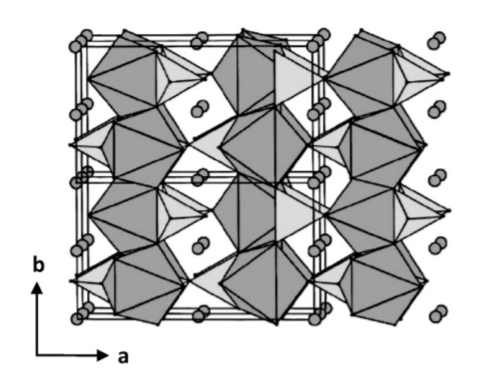
\includegraphics[width=0.6\textwidth]{LiFe.png}
\caption{$LiFePO_4$晶体结构,其中铁原子和磷原子分别占据八面体和四面体位置,锂离子嵌入其中的空隙\cite{Zhang2011Structure}} 
\label{fig:LiFe}
\end{figure}
\subsection{锂离子在两个晶体方向的输运模拟和计算}
本文的结构分析和离子扩散的计算模拟的密度泛函方法\cite{Kohn1965Self}(DFT)采用第一性计算软件包Vienna ab initio simulation package(VASP)的plane wave basis set\cite{Kresse1996Efficiency,Kresse1994Ab,Kresse1996Efficient}模拟,调用VNL进行后处理\cite{Schneider2017ATK,Stradi2017Method}和结果分析。在密度泛函计算中,利用Kohn-Sham方法将多体问题转化为一个假设虚拟粒子(如电子)在无相互作用的有效势场中运动,而粒子密度在空间中和真实系统相同的半经典近似方法\cite{Kohn1965Self}。在本文的求解中采用局域密度近似\cite{Vanderbilt1990Soft}(LDA)的求解方法进行求解。\\
\indent 首先本文进行锂离子在磷酸铁锂晶体中的扩散模拟,从而得到不同SOC的晶体结构为下一步的弹性常数的模拟和计算打好基础。
\begin{enumerate}
	\item 首先对于构建的$LiFePO_4$晶体结构进行弛豫优化:
	\begin{itemize}
		\item 采用SGGA-PBE 交换关联函数
		\item k-point取为$7 \times 5 \times 3$
		\item 应用FHI赝势和DZP基组模拟
	\end{itemize}
	具体的优化参数设定为 最大容许力为0.02 $eV/\dot{A}$,最大应力0.1$ GPa$。体系在八核CPU上耗费30分钟完成结构弛豫。
	\begin{figure}
	\centering   
	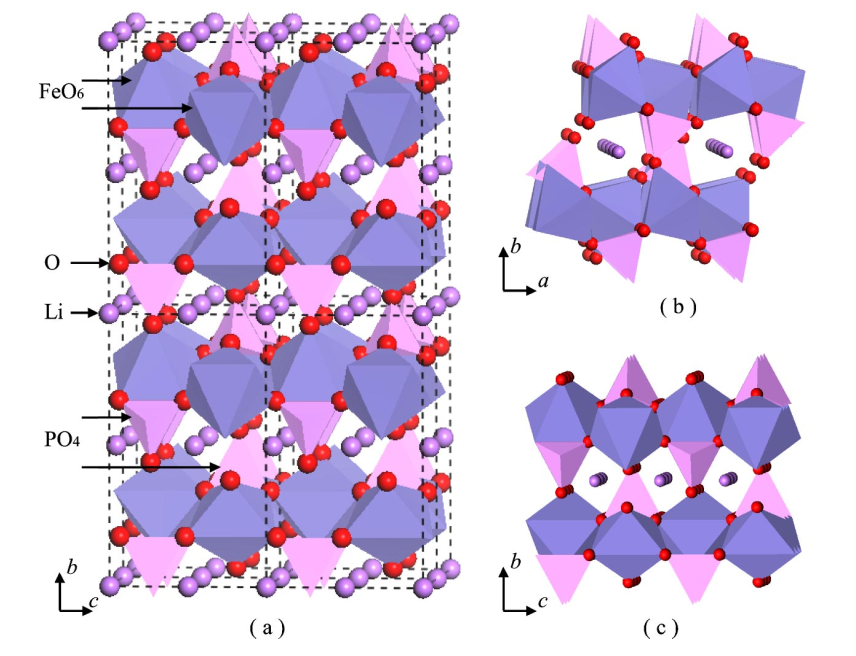
\includegraphics[width=0.6\textwidth]{diffusion.png}
	\caption{$LiFePO_4$晶体a,b,c三方向结构\cite{Ouyang2004First}} 
	\label{fig:diffusion}
	\end{figure}
	\item 文献指出,扩散势垒和锂离子的聚集形态有关\cite{Ouyang2004First},所以为了模拟锂离子的扩散过程,可以在晶格中去除四个锂离子的其中一个得到$Li_{1-x}FePO_4$的结构。如图(\ref{fig:diffusion})所示,本文将对锂离子在B,C两个方向的扩散进行研究,为此需要创建锂离子在两个方向扩散的前后的晶体构型。\\
	\begin{figure}
	\centering   
	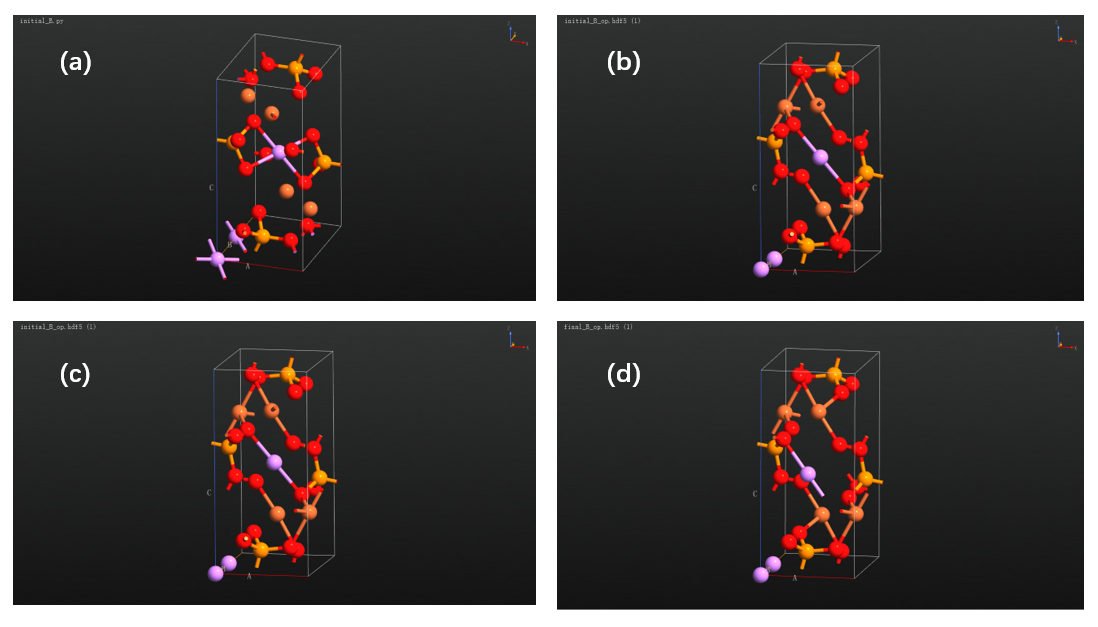
\includegraphics[width=\textwidth]{trace.png}
	\caption{$LiFePO_4$晶体B方向锂离子扩散前后结构:(a)扩散前(未优化)\quad(b)扩散前(优化后)\quad(c)扩散后(未优化)\quad (d)扩散后(优化后)}
	\label{fig:trace}
	\end{figure}
	以B方向的构型构造为例:
	\begin{enumerate}
		\item 借助引入重金属原子如Au原子得到删去某个锂原子的晶格构型,由此得到B方向的扩散的起始和终了构型的初步结构(\ref{fig:trace}(a)(c))。
		\item 对得到的两个构型的结构进行弛豫优化,需要注意的是,此处不需要对晶格常数进行优化,最后得到优化后的扩散起始和终了构型的结构(\ref{fig:trace}(b)(d))。
		\item 再通过微动弹性带方法(Nudged Elastic Band,NEB)从之前的初始构型得到扩散过程的路径和相关晶格构型\cite{Smidstrup2014Improved,Zhou2004Misfit,Kellogg1990Surface}。实际上,该方法通常需要一个基于初始和终了构型的对于可能路径的猜测而这往往是十分困难的,而实际上可以依靠自适应动力学蒙特卡洛(Adaptive Kinetic Monte Carlo,AKMC)的方法获得额外的信息从而帮助计算\cite{Xu2008Adaptive,Henkelman1999A}。对于微动弹性方法的介绍和如何应用来解决扩散路径问题的内容见附录B。
	\end{enumerate}
	\item 获得构型和扩散路径后,可以利用DFT方法计算得到其扩散过程中的能量变化,如图所示\ref{fig:energy}(a)(b):
	\begin{figure}
	\centering   
	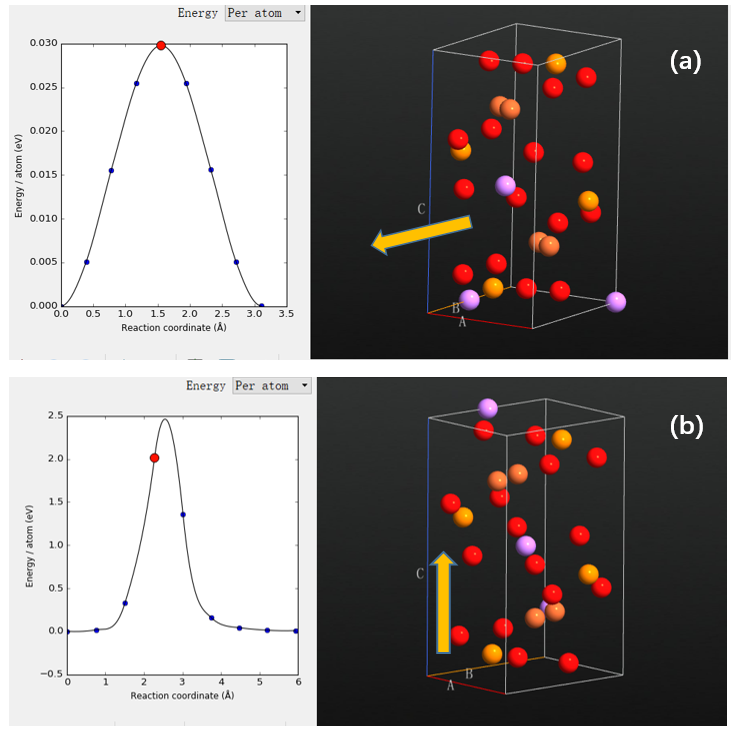
\includegraphics[width=0.8\textwidth]{energy.png}
	\caption{$LiFePO_4$晶体B方向和C方向锂离子扩散过程} 
	\label{fig:energy}
	\end{figure}
	可以看出,由于较小的势垒,锂离子在B方向的扩散要比在C方向扩散要容易很多。
	\item 基于前面对于扩散过程能量势垒的研究,从微观上而言,锂离子的扩散主要依赖势垒高低,从宏观上而言,这一参数可以用电化学反应的速率来很好的描述。基于此,本文采用谐波过渡态理论(Harmonic Transition State Theory,HTST)来计算两个扩散方向的反应速率\cite{Vineyard1957Frequency,Eyring1935The,Voter1984Transition}(较为详细的计算过程见附录B)。两个方向的结果见图\ref{fig:reaction},可以看出B方向的反应速率远远高于C方向,和微观的势垒分析的结果一致。
	\begin{figure}
	\centering   
	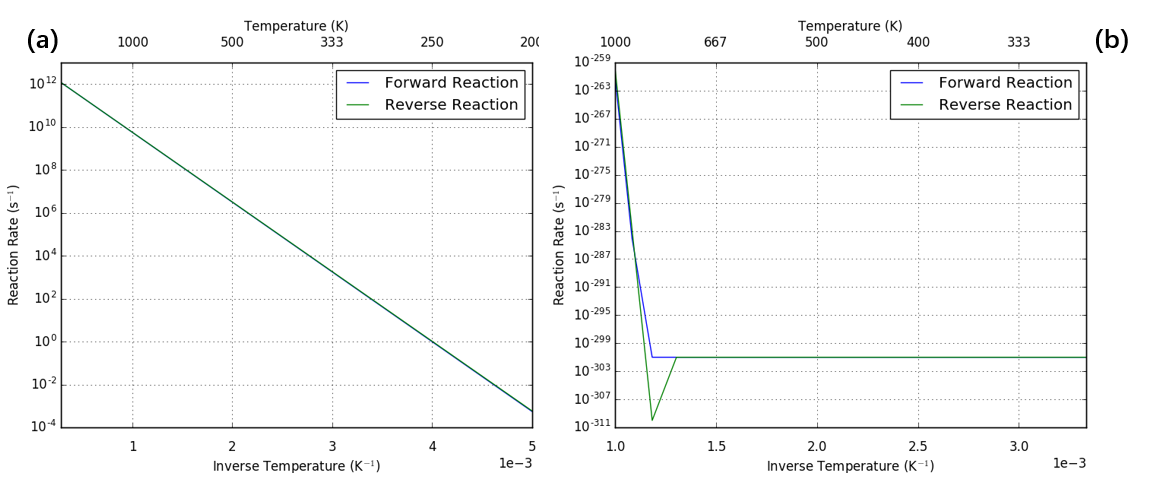
\includegraphics[width=\textwidth]{reaction.png}
	\caption{$LiFePO_4$晶体B方向和C方向反应速率图:(a)B方向 (c)C方向} 
	\label{fig:reaction}
	\end{figure}
\end{enumerate}
\indent以上基于第一性原理对于锂离子在$LiFePO_4$晶体B和C两个方向的扩散输运的在300k下的势垒和反应速率可以总结如表\ref{tab:HTST}:
\begin{table}[!htbp]
\centering
\caption{势垒和反应速率}\label{tab:HTST}%添加标题 设置标签
\begin{tabular}{ccc}
\toprule
Direction & Barrier(eV) & $k_{HTST}$\\
\midrule
B & 0.03 & $2.5 \times 10^6$\\
C & 2.5 & $10^{-300}$ \\
\bottomrule
\end{tabular}
\end{table}

\subsection{弹性常数的计算及各向异性分析}
\subsubsection{线弹性关系}
对于晶体而言,其在一定的范围内都很好的满足线弹性的关系,则应力和应变都是二阶张量,其在空间中均有九个分量,可以用Voigt notation表示为下列形式:
\begin{equation}
\label{eq:stress}
\mathbf{\sigma} =\left( \sigma_{xx}, \sigma_{yy}, \sigma_{zz}, \sigma_{yz}, \sigma_{xz}, \sigma_{xy} \right)
\end{equation}
\begin{equation}
\label{eq:strain}
\mathbf{\epsilon} =\left( \epsilon_{xx}, \epsilon_{yy}, \epsilon_{zz}, 2\epsilon_{yz}, 2\epsilon_{xz}, 2\epsilon_{xy} \right)
\end{equation}
由张量理论,应变张量和应力张量之间由弹性矩阵相关联,弹性矩阵为一个四阶张量,表现为一个$6 \times 6$的矩阵,其中的元素称为弹性常数。
\begin{equation}
\label{eq:rule}
\mathbf{\sigma} = \mathbf{C} \cdot \mathbf{\epsilon} 
\end{equation}
由于晶体均有对称性,所以很多时候,弹性矩阵中的独立参数的数目可以被缩减。比如,对于立方晶系而言,只有$C_{11}$,$C_{12}$,$C_{44}$是独立的,此时方程\ref{eq:rule}可以简化为:
\begin{equation}
\begin{pmatrix}
\sigma_1\\
\sigma_2\\
\sigma_3\\
\sigma_4\\
\sigma_5\\
\sigma_6\\
\end{pmatrix}
=
\begin{pmatrix}
C_{11} & C_{12} & C_{12} & 0 & 0 & 0\\
C_{12} & C_{11} & C_{12} & 0 & 0 & 0\\
C_{12} & C_{12} & C_{11} & 0 & 0 & 0\\
0&0&0& C_{44} & 0 & 0\\
0&0&0& 0 &C_{44} & 0 \\
0&0&0& 0 & 0& C_{44} \\
\end{pmatrix}
\begin{pmatrix}
\epsilon_1\\
\epsilon_2\\
\epsilon_3\\
\epsilon_4\\
\epsilon_5\\
\epsilon_6\\
\end{pmatrix}
\end{equation}
\subsubsection{模拟过程}
\indent 在模拟中,为了求解得到弹性常数,首先在选定的方向给定晶格微小的形变,如$\mathbf{\eta}$,然后求解产生的应力向量。然后再对每一个应变向量下的应力分量$\sigma_i(\eta)$做拟合,这样就可以再通过求解一系列的考虑了具体晶格结构的线性方程组的最小二乘解得到所相互独立的弹性常数。在计算中,模拟程序实际采用的是文献所推荐的计算弹性常数的ULICS方法\cite{Yu2010Calculations},即每一个参考点,所给定的初始变形为$(-\eta,0,\eta)$。\\
\indent 实际上,在单轴加载的情况下$(\epsilon_{22}=\epsilon_{33}=0,\epsilon_{11} \not \eq 0)$,x方向的应力就可以表示为:
\begin{equation}
\sigma_{11} = C_{11}\epsilon_{11}
\end{equation}
进而可以计算体弹模量 $K$ 为:
\begin{equation}
K = \frac{1}{3} \left(\frac{\sigma_{11}+\sigma_{22}+\sigma_{33}}{\epsilon_{11}+\epsilon_{22}+\epsilon_{33}} \right)
\end{equation}
可以看出,可以建立弹性常数$C_{11}$和体弹模量$K$和应力应变的关系,从而进一步可以得到$C_{11}$和$K$和宏观材料力学参数杨氏模量和泊松比的关系(对于各向同性材料而言):
\begin{equation}
\label{eq:C11}
C_{11} =\frac{(1- \nu)E}{(1+\nu)(1-2\nu)}
\end{equation}
\begin{equation}
\label{eq:K}
K = \frac{E}{3(1-2\nu)}
\end{equation}
从方程\ref{eq:C11}和\ref{eq:K}可以得出,等效杨氏模量可以由下式求得:
\begin{equation}
E = \frac{9K(C_{11}-K)}{3K + C_{11}}
\end{equation}
\indent 弹性常数的第一性原理模拟中涉及具体模拟参数的设置,讨论如下:
\begin{itemize}
	\item $\mathbf{\eta_{max}}$ \\
	表征了对晶格所施加的最大变形,显然,只要限制在线弹性的区域内,相对较大的变形会得到比较好的应力变化从而得到比较准确的弹性常数。 根据之前的对于晶体的计算经验,通常而言默认取值为$\eta_{max} = 0.002$。
	\item $\mathbf{\eta_{\eta}}$\\
	该参数为施加变形场时的差分间隔,即可以通过$\eta_{\eta}$和$-\eta_{max},\eta_{max}$求得所需要具体计算的每一个形变量。 当然,采用相对密集的取点(即相对比较小的$\eta_{\eta}$的取值)和高阶的插值函数可以增加精度。但是由于此处不需要模拟非线性(如塑性)行为,只需要取到$\eta_{\eta}=3$即可。
\end{itemize}
\subsubsection{计算结果和分析}
由于本文研究锂离子扩散过程对路径基于NEB方法进行了详细而比较准确的模拟,所以可以得到整个扩散过程的晶体构型,从而可以分别对每一个构型进行弹性常数的计算。需要指出的是,由于电极材料所面临的核心难题为锂离子在扩散过程中电极材料的断裂,所以对于扩散过程和力学特性进行耦合研究显得十分必要,特别是,基于本文的研究思路的方法,可以得到电极活性材料(此处为$LiFePO_4$)随着锂离子的扩散而产生的力学特性的动态变化,从而进行下一步的耦合研究和分析建模。\\
\begin{figure}
	\centering   
	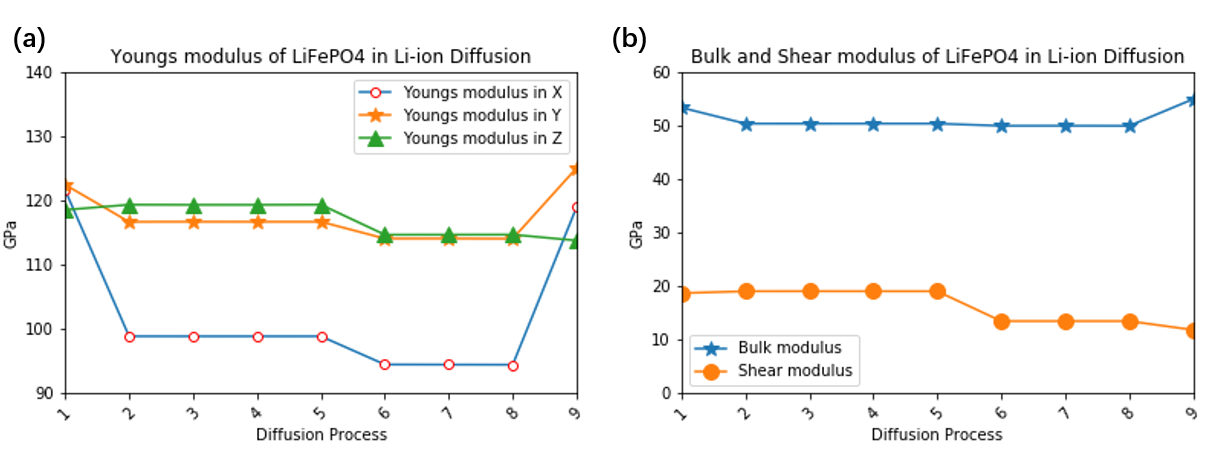
\includegraphics[width=\textwidth]{modulus.png}
	\caption{$LiFePO_4$晶体在锂离子扩散过程中其三个方向弹性模量和体弹模量和剪切模量的变化} 
	\label{fig:modulus}
\end{figure}
\indent 如图\ref{fig:modulus}所示,本文分析了在锂离子沿着B方向扩散过程中晶体的弹性参数的变化,可以看出在锂离子的扩散行为和晶体的力学特性的耦合特性。具体分析发现,其模量基本上都在扩散过程中有着下降的趋势,可能是由于扩散时成键较弱此时抵抗外界变形的能力相对减弱,从而其模量变小。定量的分析可以发现,在整个扩散过程中,三个方向的杨氏模量分别最小为之前的$77.65\%$,$91.18\%$和$95.32\%$,也就是说其模量会有最高$23\%$的减小。\\
\indent 另一方面,对弹性常数的计算分析可以知道,$LiFePO_4$晶体有着很强的力学各向异性。 而研究指出,作为锂离子电池的电极材料,随着锂离子在其中的扩散,由于其各向异性,会促使裂纹的形成和发展\cite{Tvergaard1988Microcracking,Rice1992Dislocation},从而使得电极活性材料失效乃至电池容量减退。对正交晶系的材料而言,其各向异性分为剪切产生和各向体弹模量非线性产生,
一般可以定义以下三个各向异性因子进行表征\cite{Ranganathan2008Universal,Ravindran1998Density}:
\begin{equation}
A_1 = 4c_{44}/(c_{11} + c_{33} -2c_{13})
\end{equation}
表征\{100\}平面的<010>和<011>方向
\begin{equation}
A_2 = 4c_{55}/(c_{22} + c_{33} -2c_{23})
\end{equation}
表征\{010\}平面的<001>和<101>方向
\begin{equation}
A_3 = 4c_{66}/(c_{11} + c_{22} -2c_{12})
\end{equation}
表征\{001\}平面的<010>和<110>方向\\
\indent 选取扩散过程中的四个代表结构进行三个各向异性因子的计算,其结果见表\ref{tab:A},同时也利用\cite{jerkwin}提供的各向异性晶体弹性常数可视化的方法绘制出以上四个结构的各向异性图示\ref{fig:mat}。
\begin{table}[!htbp]
\centering
\caption{各向异性系数}\label{tab:A}%添加标题 设置标签
\begin{tabular}{cccc}
\toprule
Sample & $A_1$ & $A_2$ & $A_3$\\
\midrule
1 & -2.0899 & 0.5637 & 0.4491\\
2 & -2.1834 & 1.0742 & 0.4423 \\
3 & -2.7376 & 1.0575 & 0.3800\\
4 & -2.7480 & 0.9571 & 0.4618\\
\bottomrule
\end{tabular}
\end{table}

\begin{figure}
  \centering
  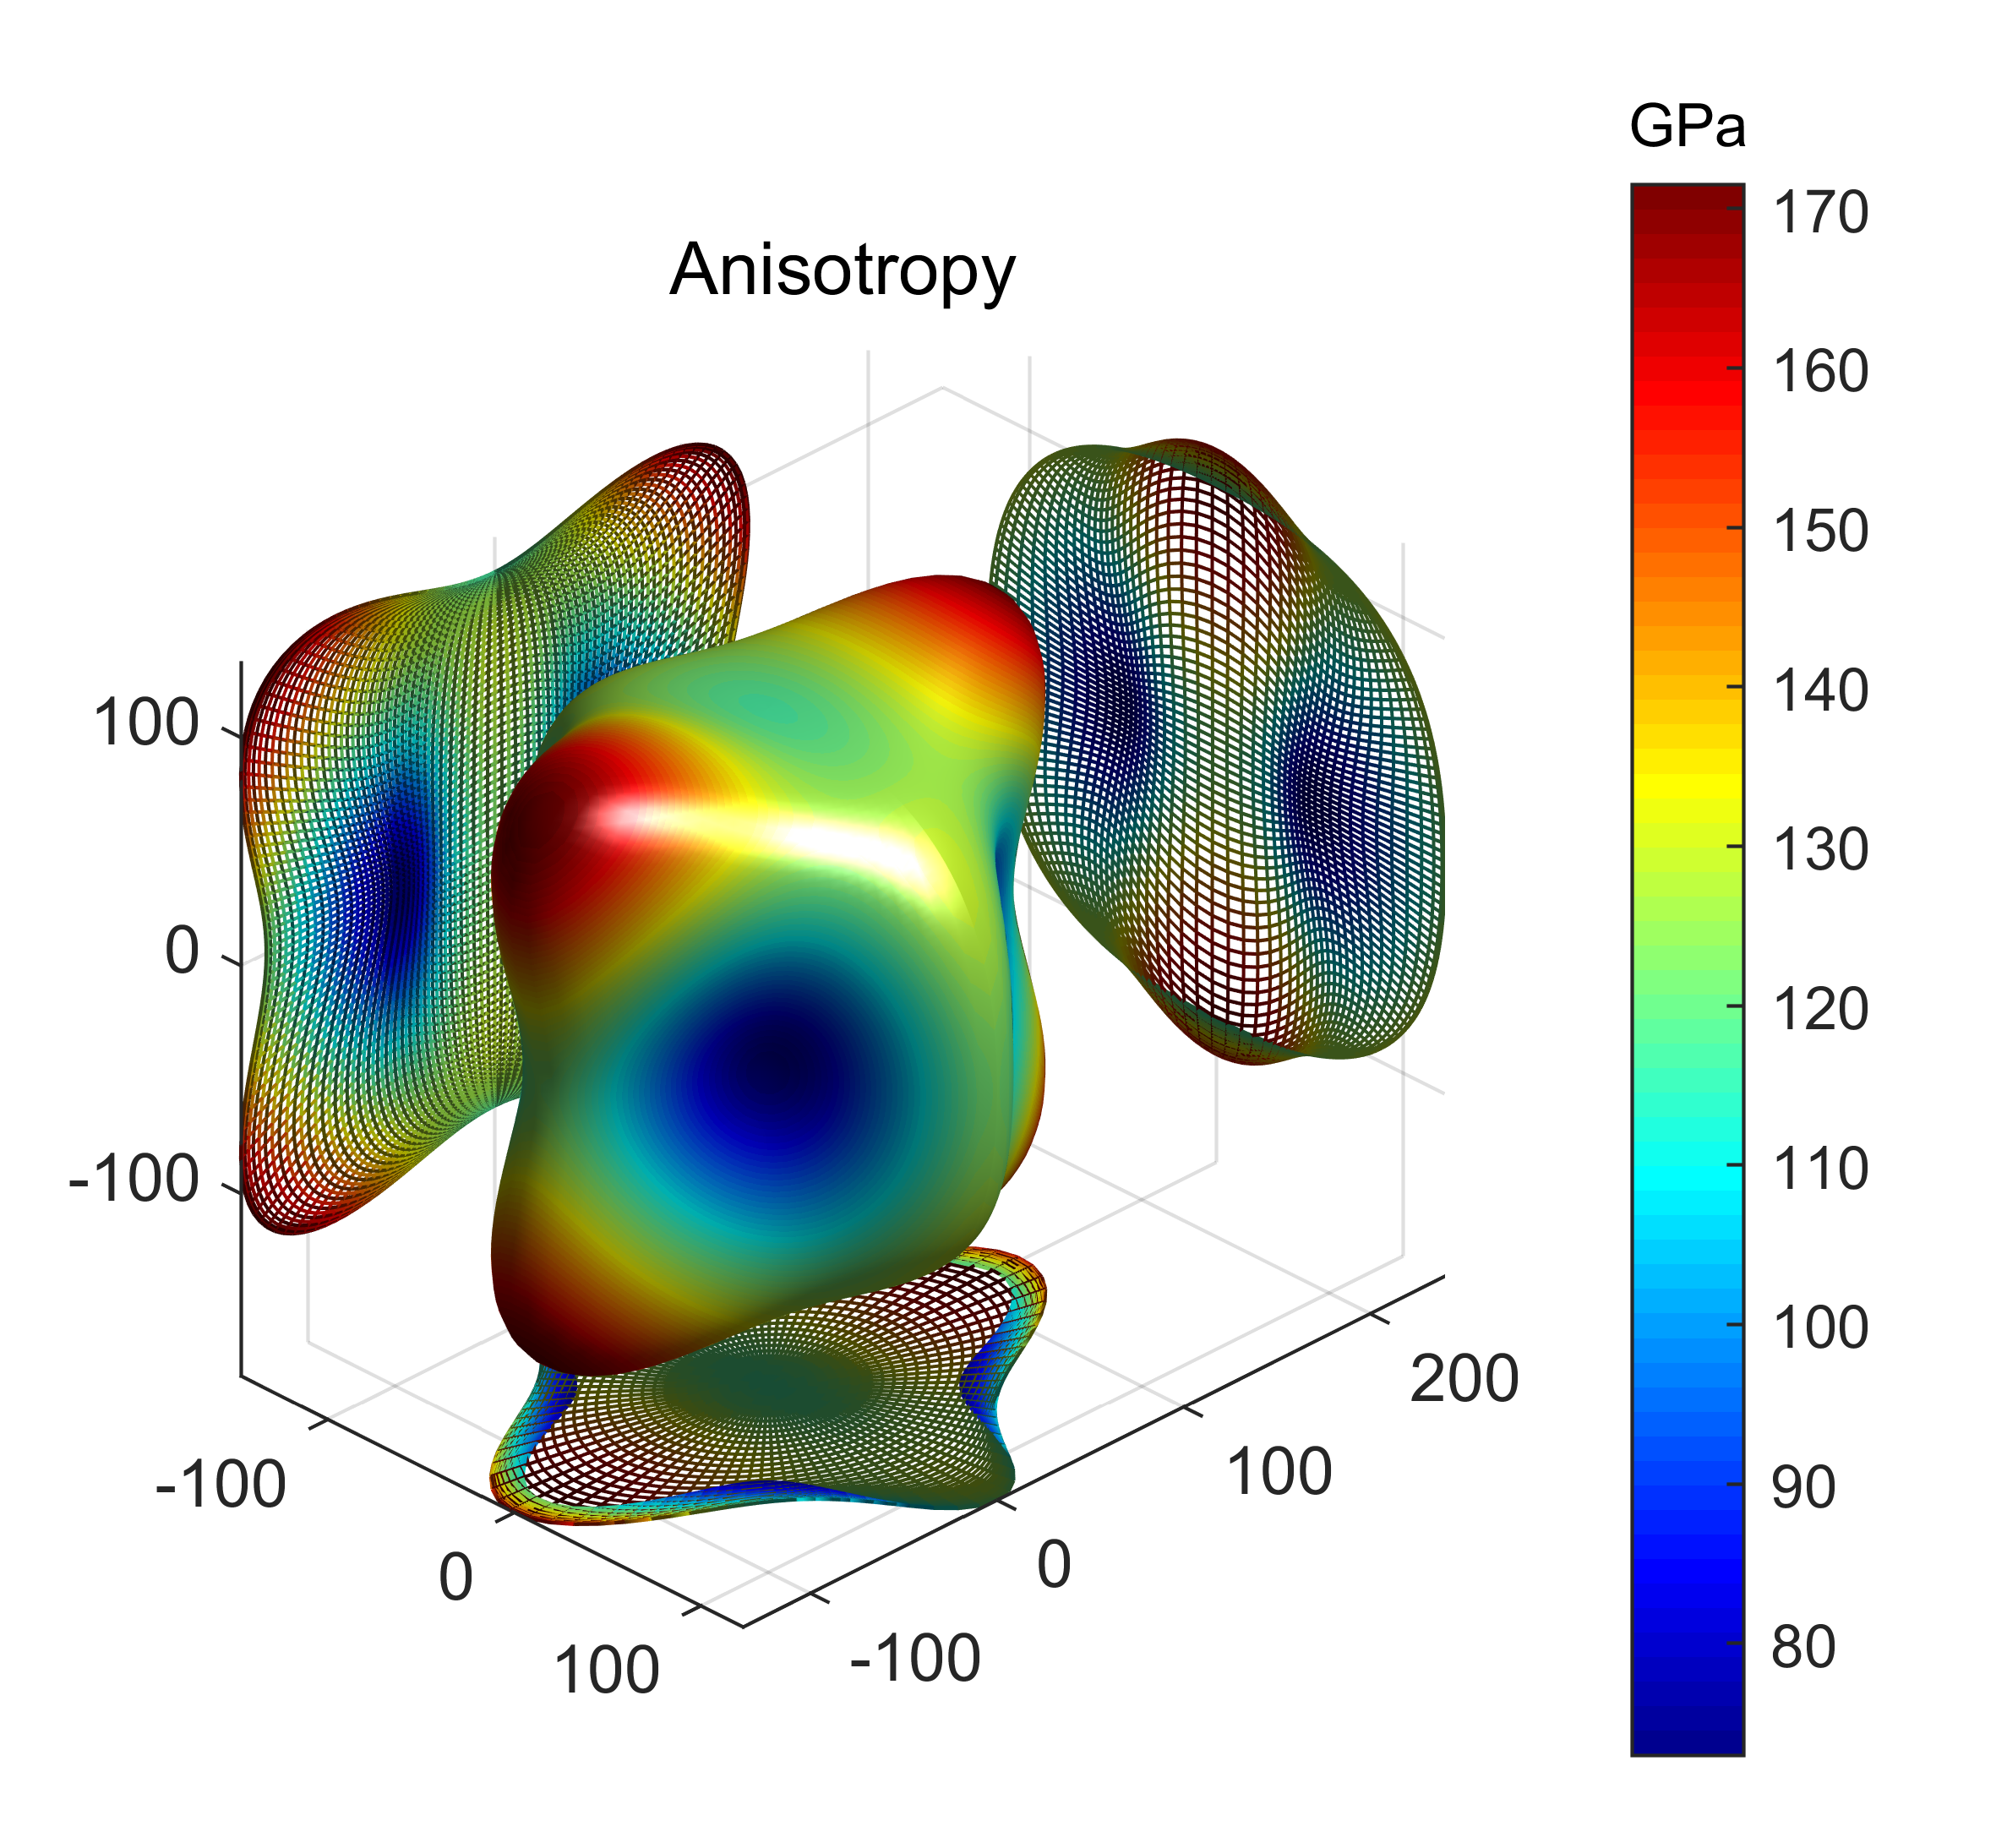
\includegraphics[width=.4\linewidth - 0.25mm]{1.png}\hfill
  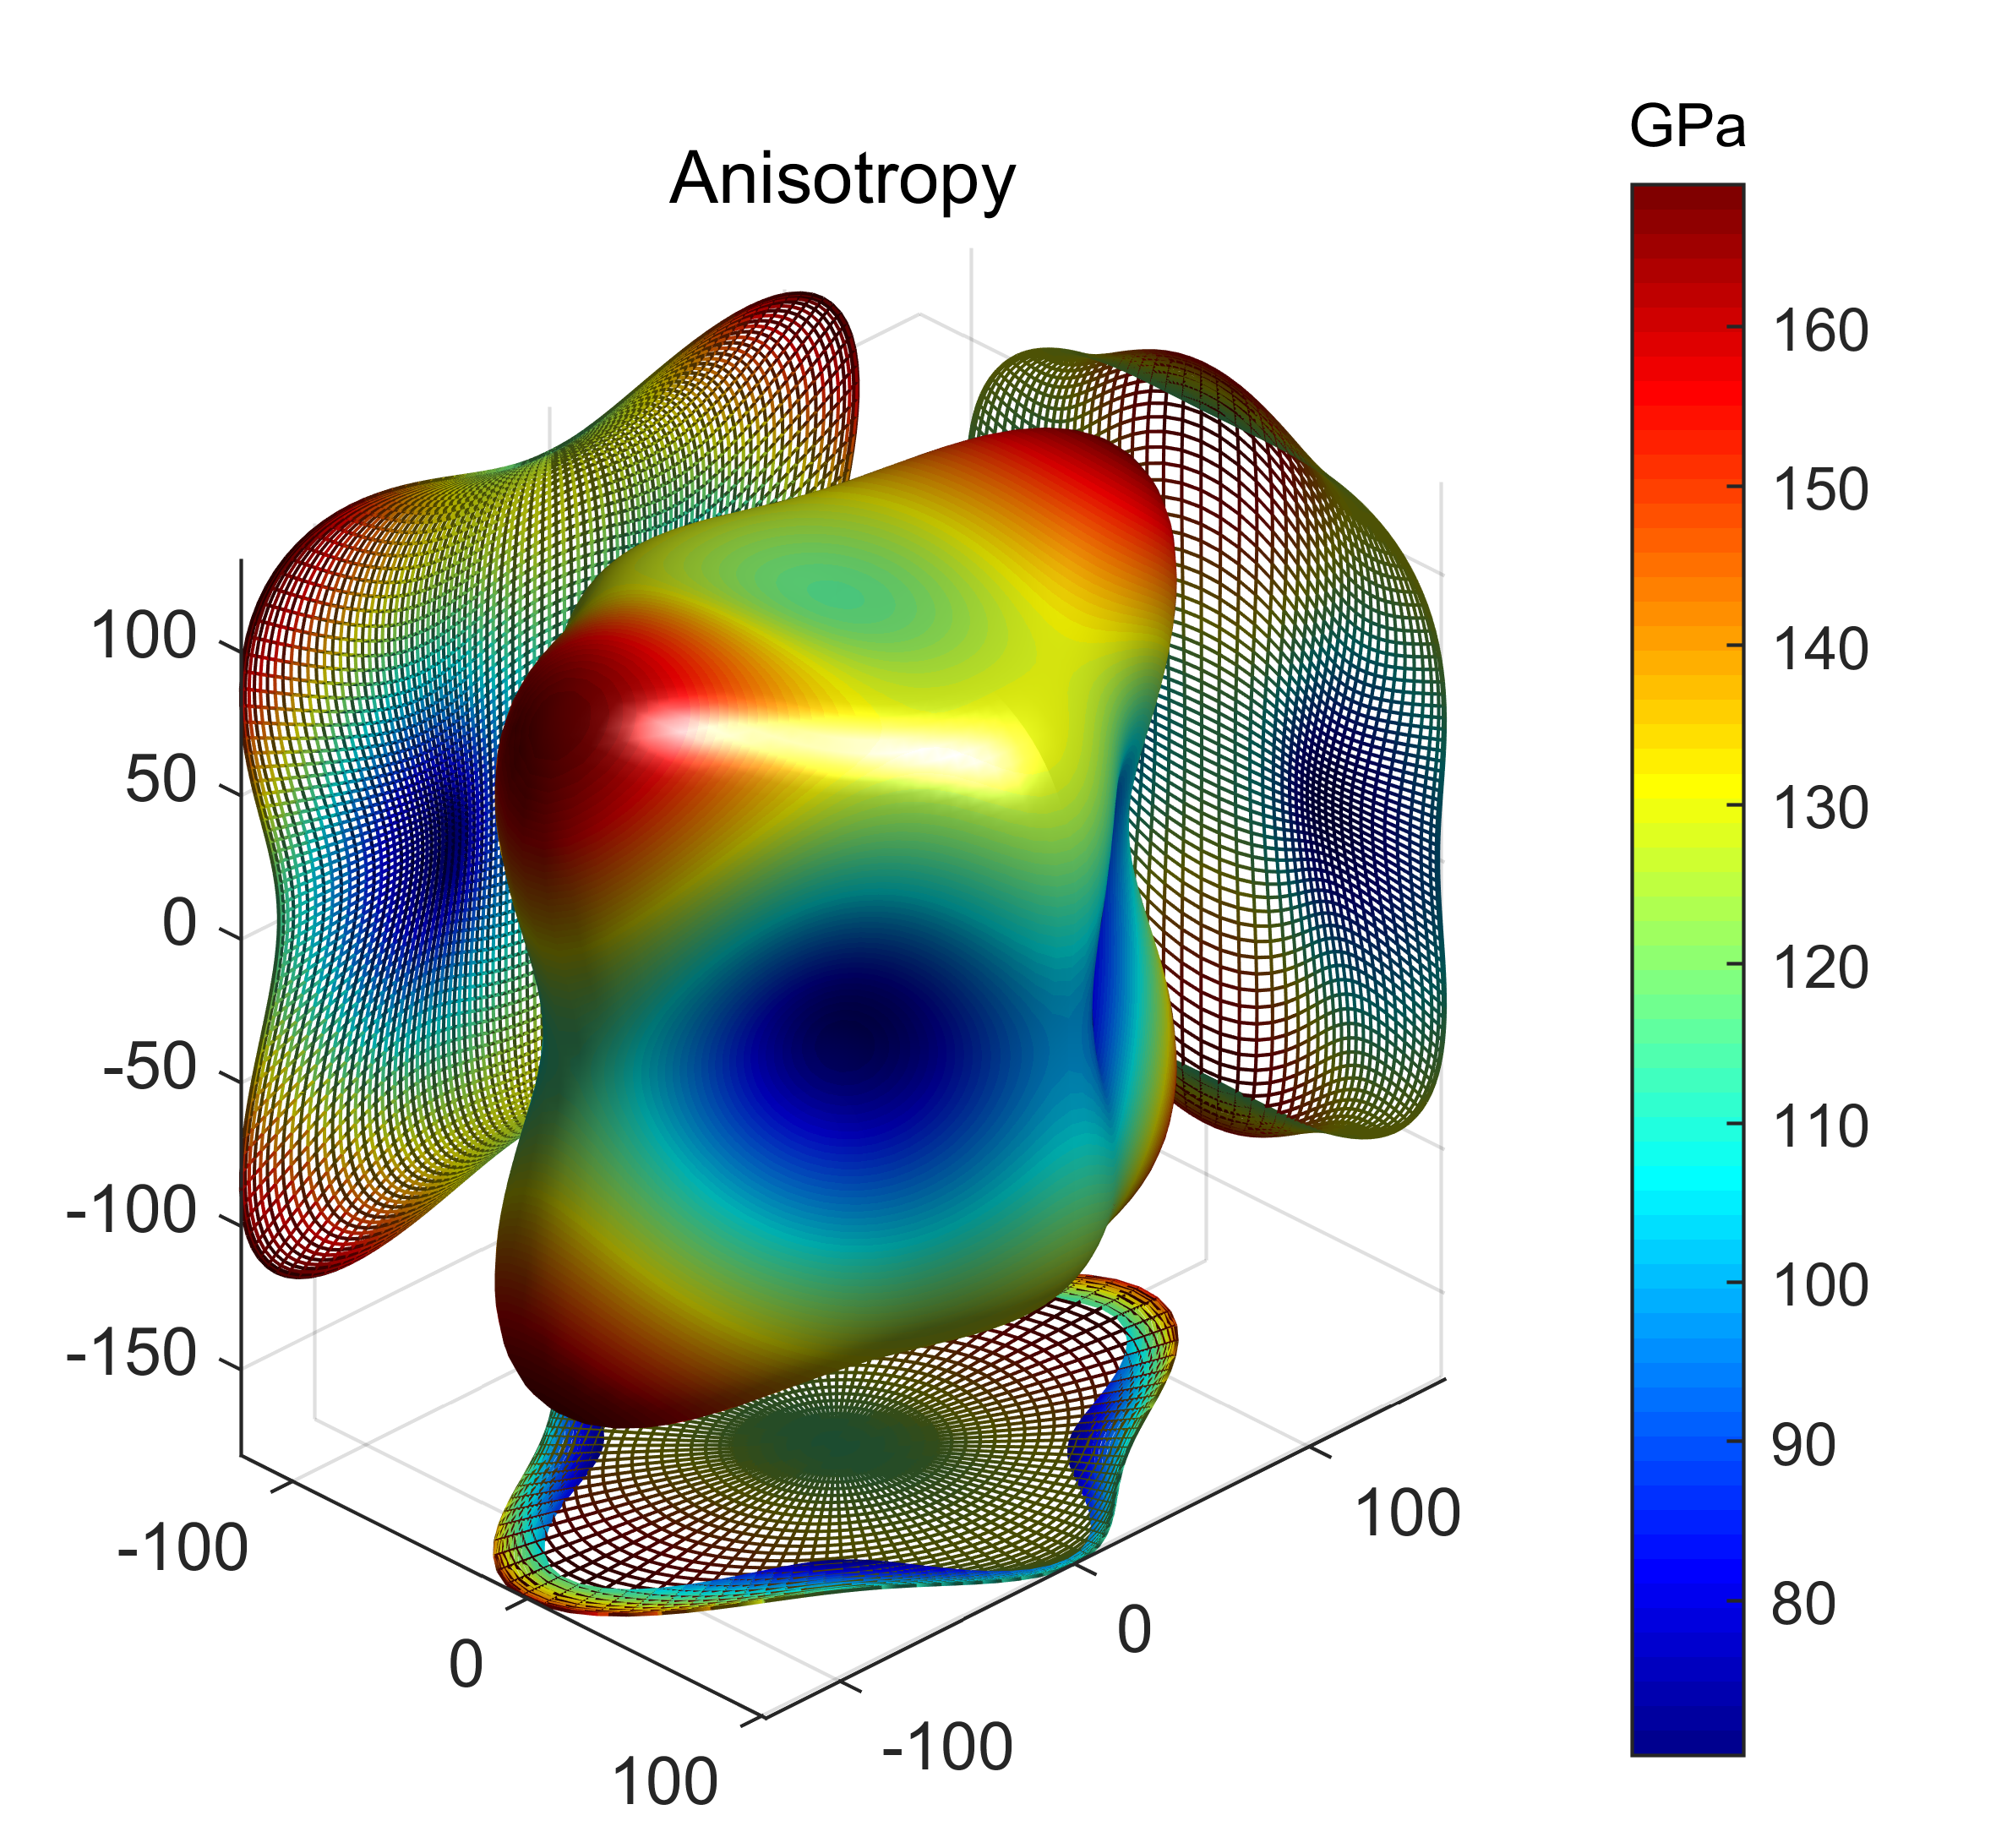
\includegraphics[width=.4\linewidth - 0.25mm]{2.png}\\[0.5mm]
  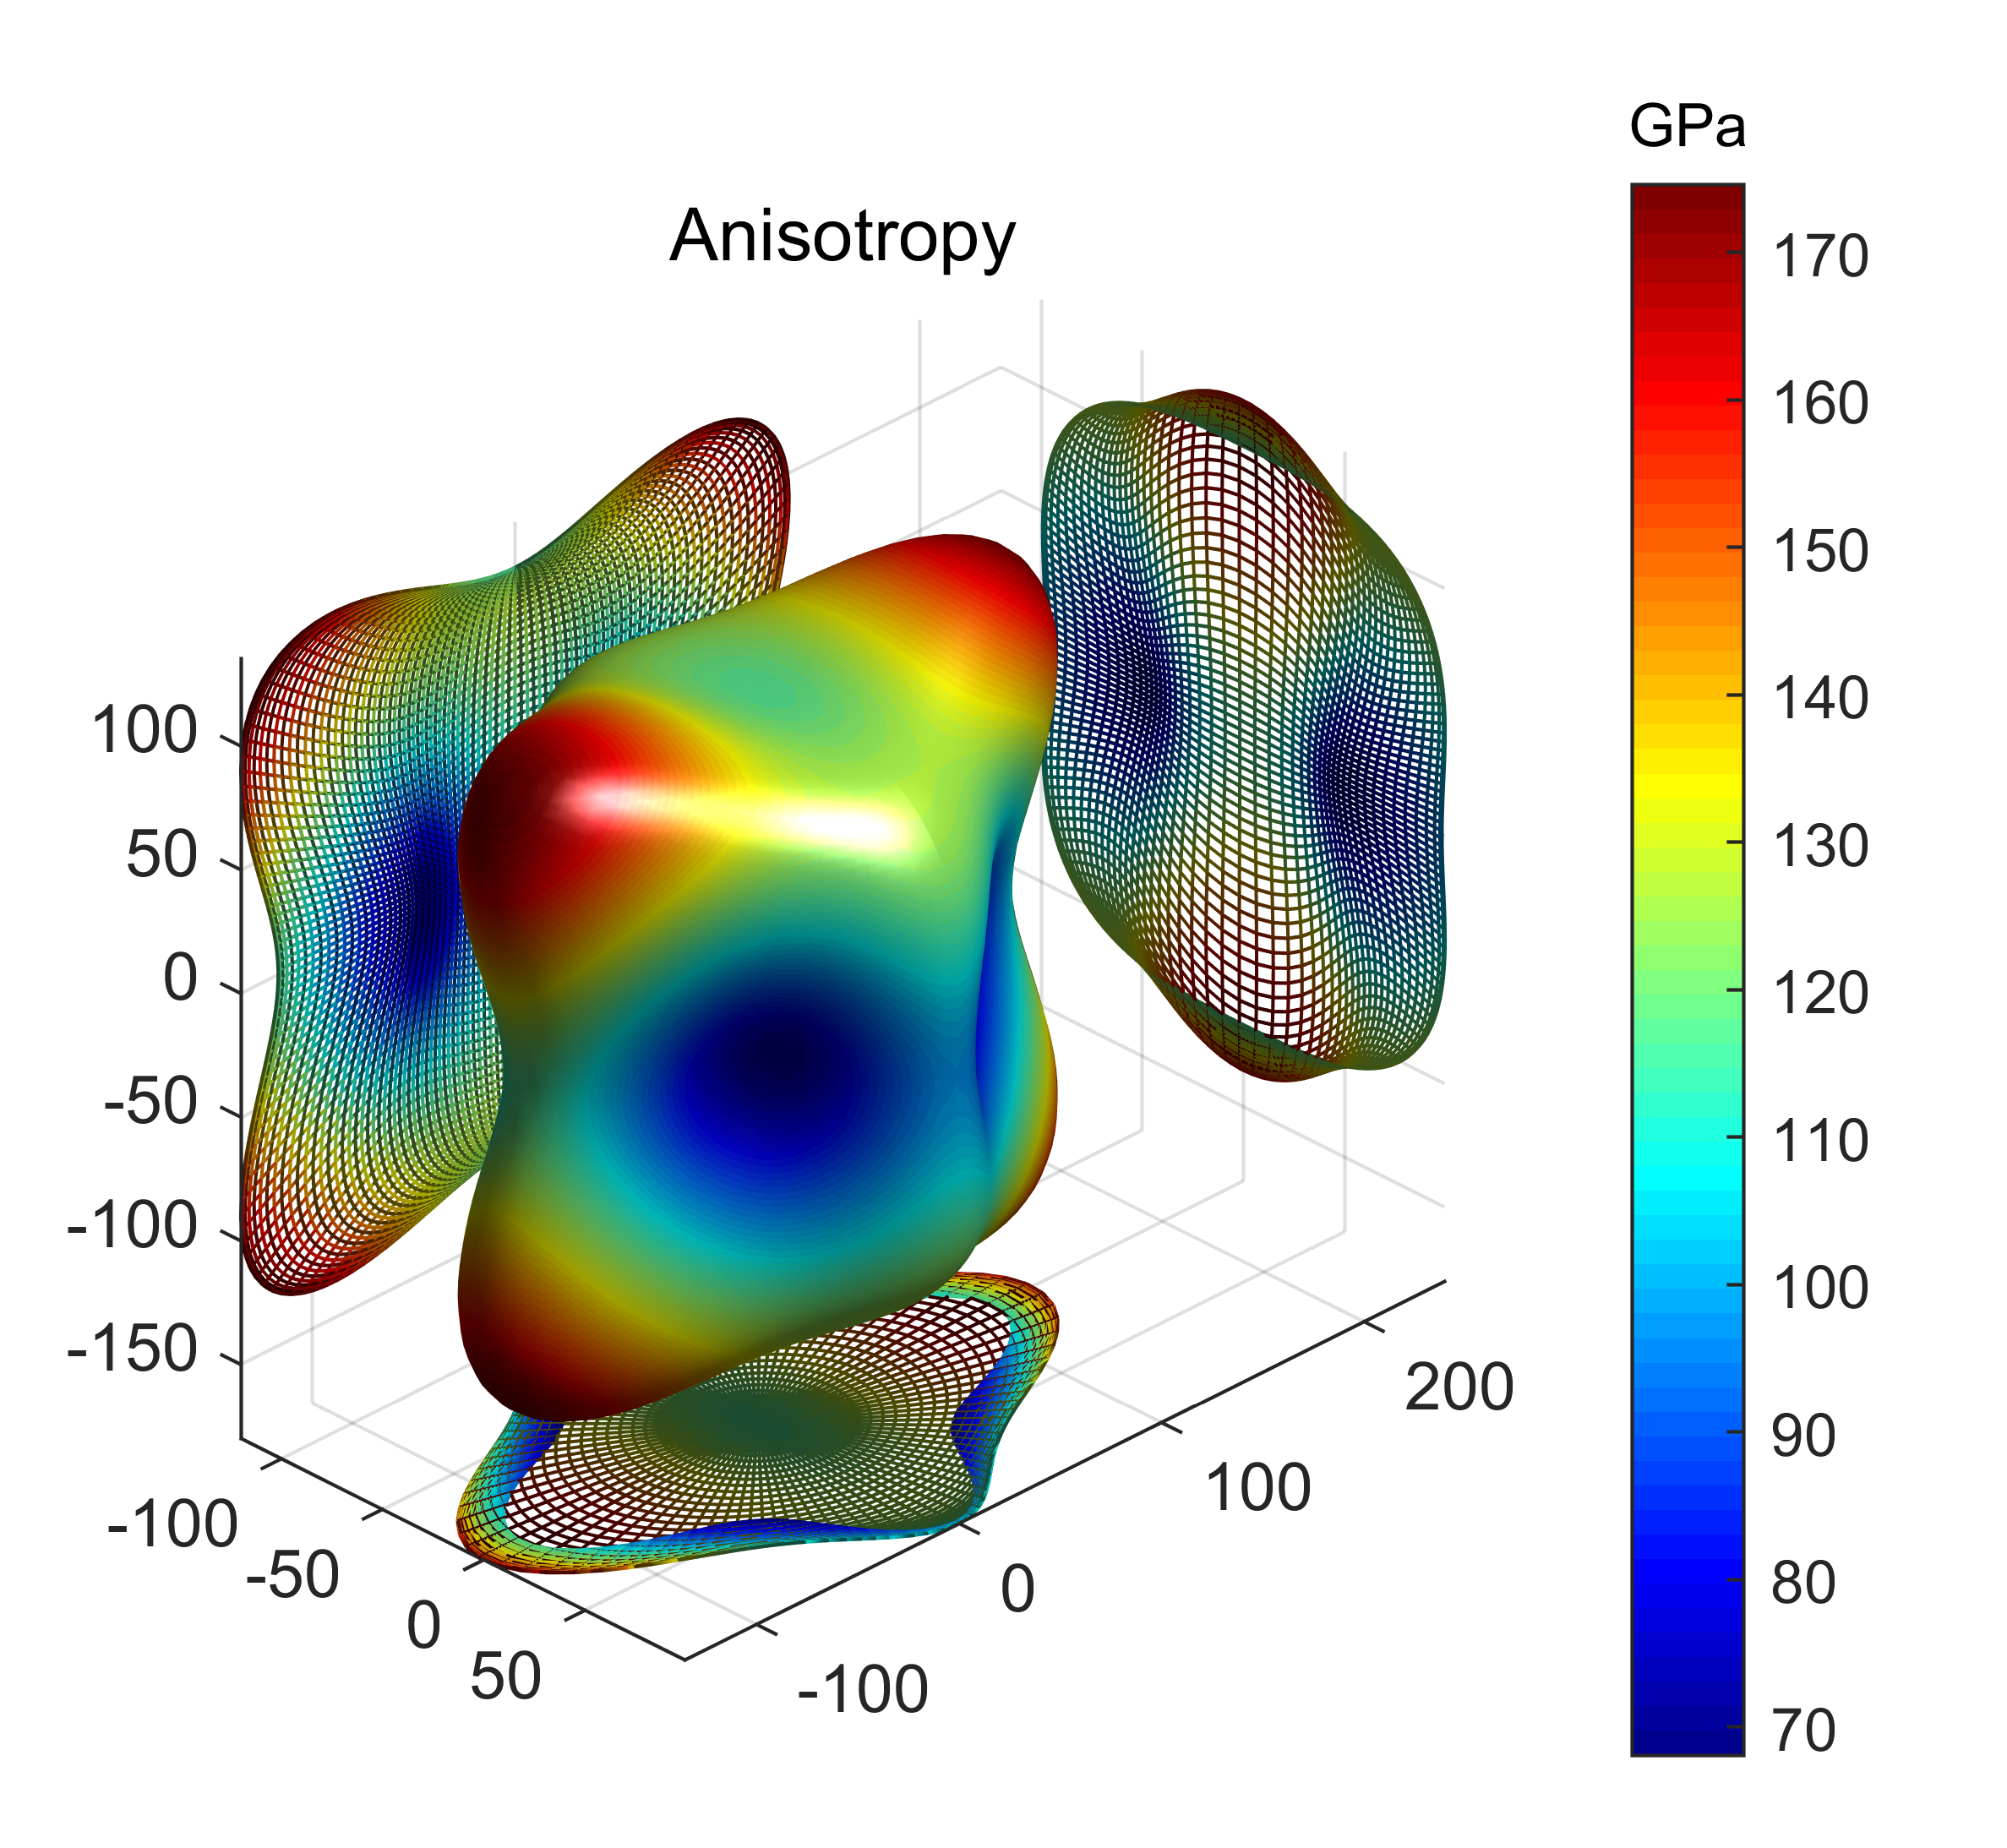
\includegraphics[width=.4\linewidth - 0.25mm]{3.png}\hfill
  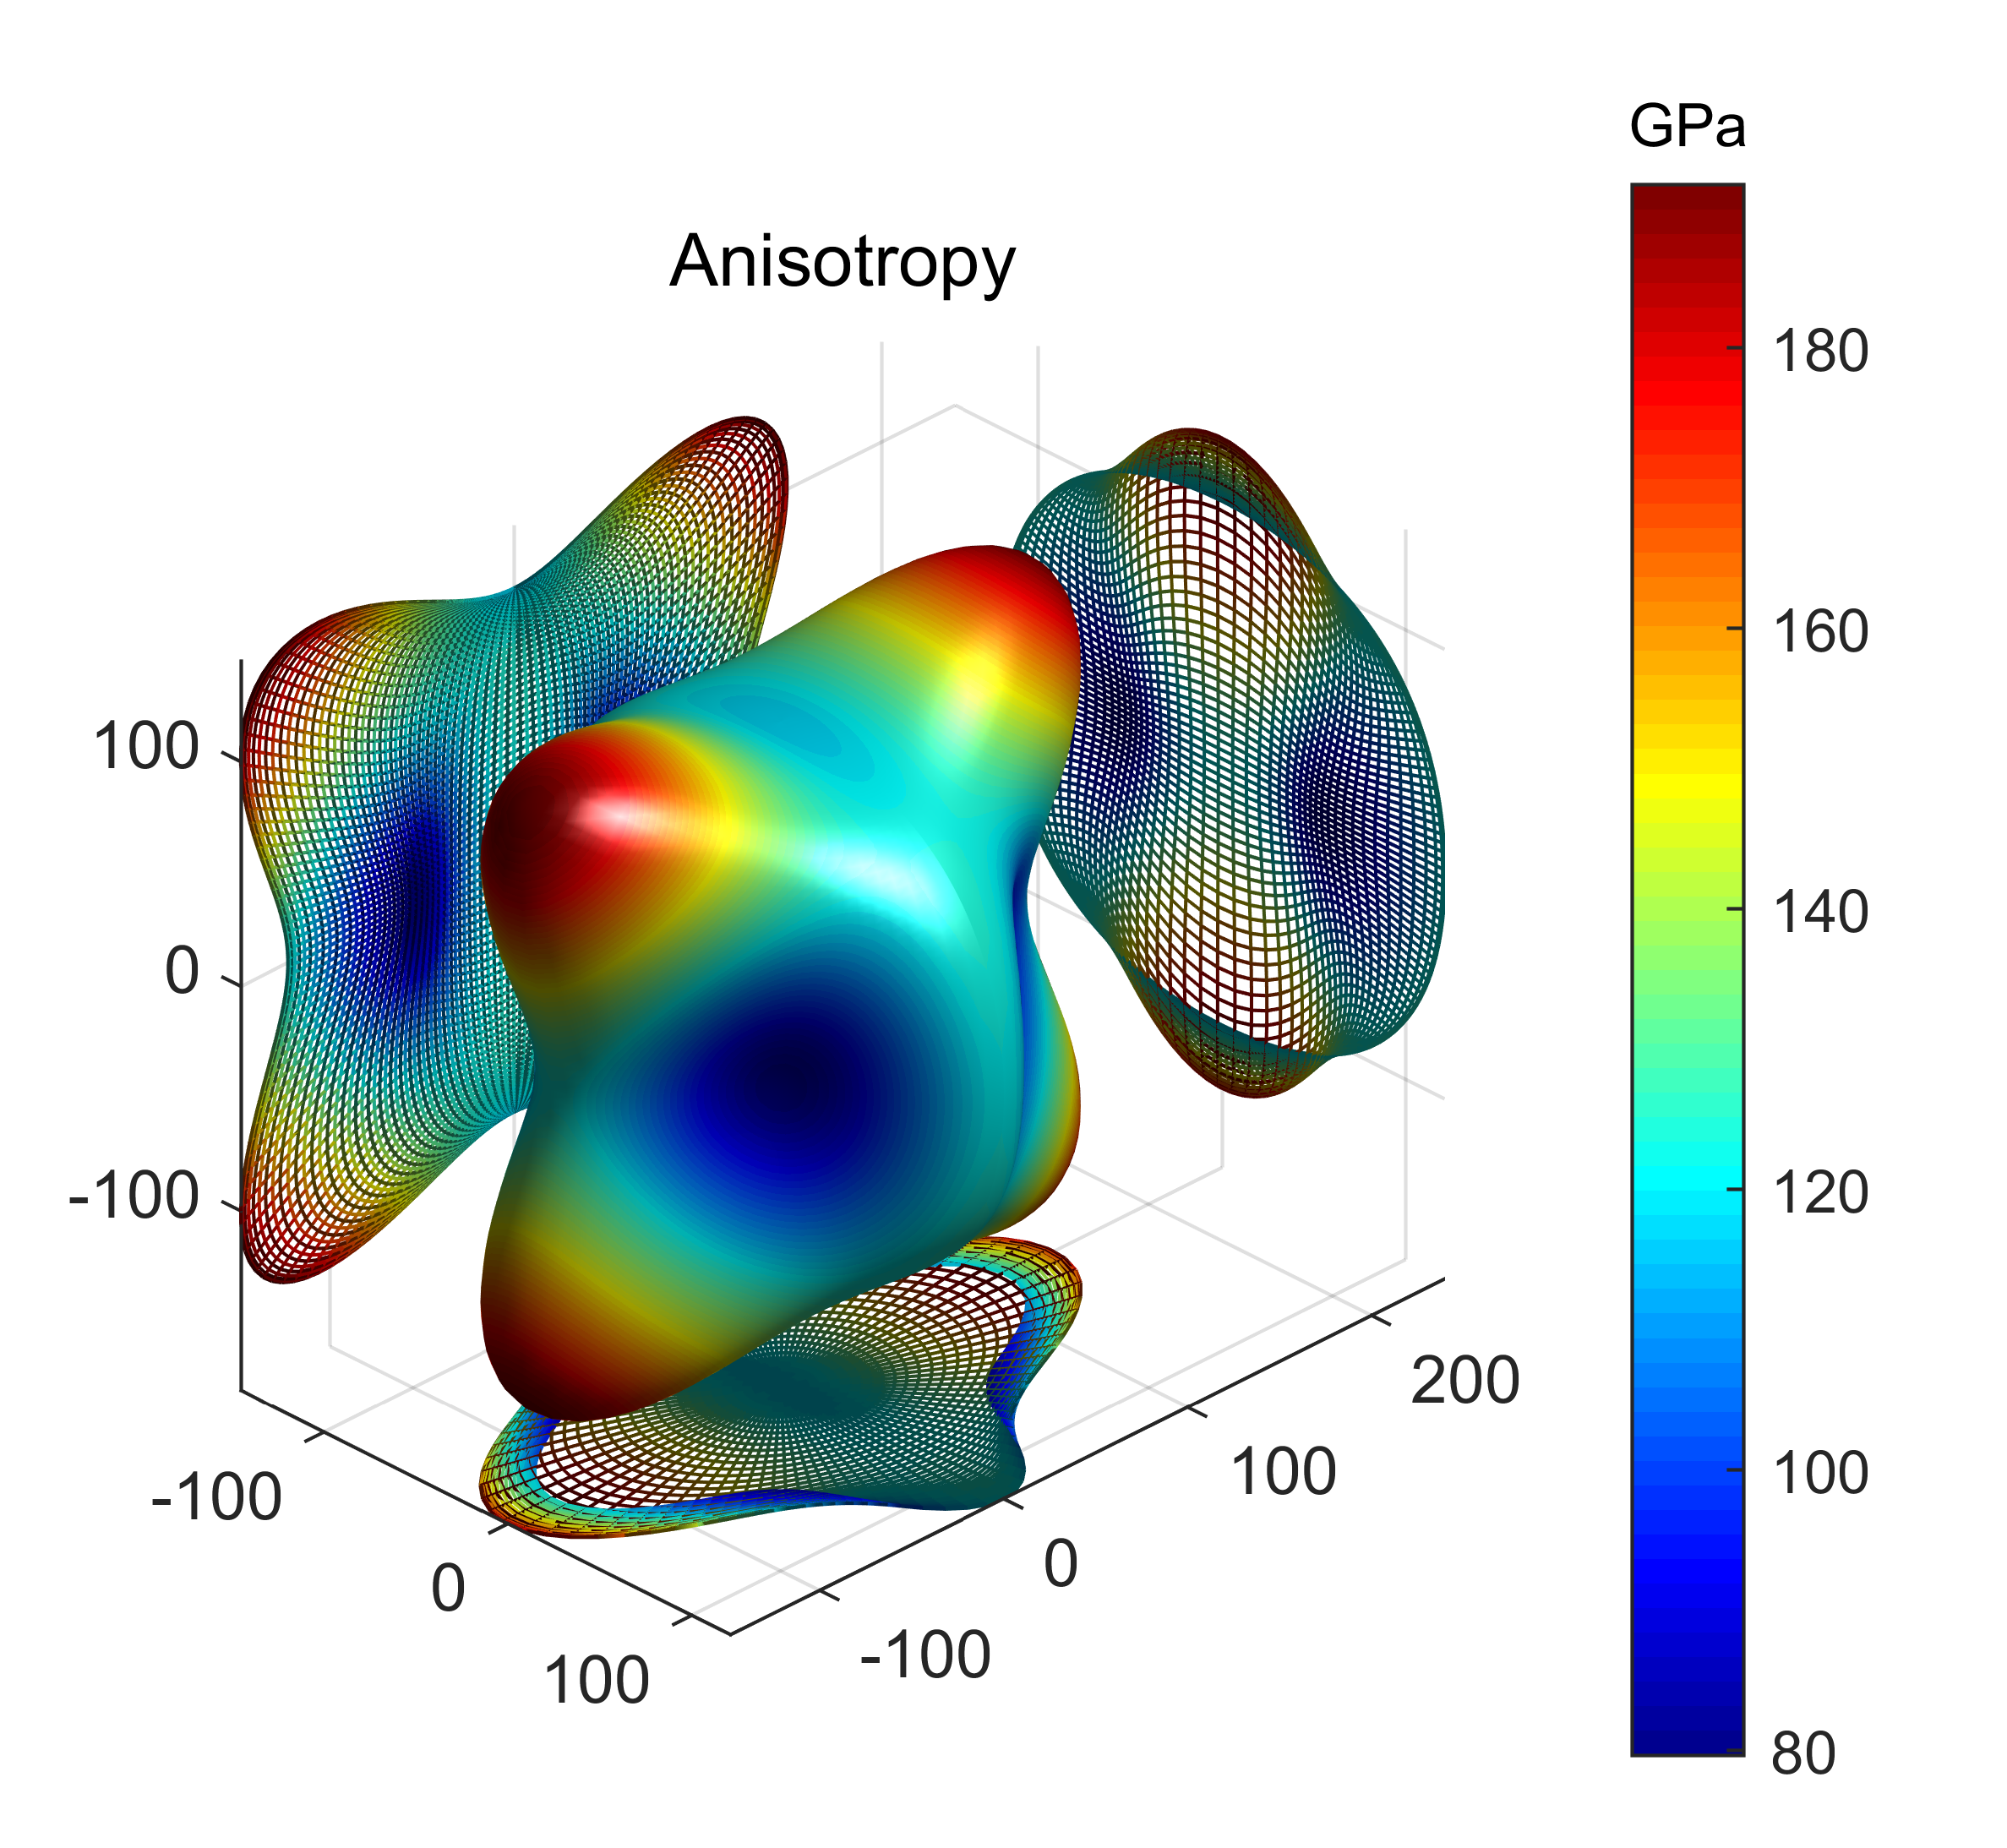
\includegraphics[width=.4\linewidth - 0.25mm]{4.png}
  \caption{$LiFePO_4$晶体在锂离子扩散过程中其三个方向弹性模量和体弹模量和剪切模量的变化} 
	\label{fig:mat}
\end{figure}

\section{不同SOC下的$LiFePO_4$晶体力学响应的模拟研究:分子动力学模拟}
\subsection{模拟方法:分子动力学计算}
由于控制不同的SOC\cite{Qi2010Threefold}和制备磷酸铁锂大单晶十分困难,$LiFePO_4$的力学特性对于不同SOC的依赖特性少有实验研究。而分子动力学模拟则是求解这一问题的有效手段。另外,锂离子的扩散引起的体积变化的直接效应是引起一个应变场,从而采用应变加载的方式对于体系进行力学响应研究也可以模拟体积变化的影响。\\
\indent 前文对锂离子扩散过程中的弹性特性进行研究,通过第一性原理计算的方法得到了锂离子扩散过程中的不同阶段晶格的弹性常数并以之为基础得到了弹性参数,总结出了电化学和力学所耦合的规律,而这里本文将对晶体结构的外力加载的力学响应行为进行模拟,主要得到其失效特性以及其塑性行为。而对这一问题,分子动力学由于其适应相对较大的体系研究,计算速度较快和计算效率较高的特点很适合这一问题的模拟和研究。需要指出的是,除了有着相对较快的计算速度和相对较大的模拟规模,在分子动力学模拟中,由于体系能量,应力等物理量都是分子坐标的光滑和连续函数,使得对于预先给定应变求解应力的算法有着很好的稳定性。\\
\indent  首先,本文对之前的扩散研究得到锂离子扩散前后的晶格构型进行弛豫。 需要指出的是,由于磷酸铁锂结构的复杂性,需要对每一种构型进行足够时间的弛豫。与基于量子力学的计算相比,由于预先定义的经验势能,所以计算的成本大为下降,可以在可以接受的时间和空间成本的花费下进行相对较大体系的模拟。\\
\subsubsection*{分子动力学}
分子模拟的势能项采用考虑了(1)长程作用的Coulomb势能 (2)短程作用的Morse函数 (3)附加项 $C/r^{12}$,呈现以下形式\cite{Alfonso2006A}:
\begin{equation}
\label{eq:MD}
U(r) = \frac{z_i z_j e^2}{r} +D_{ij} \left[\{1-e^{-a_{ij}(r-r_0)}\}^2 -1 \right] + \frac{C_{ij}}{r^{12}}
\end{equation}
\\
其中,第一项表征了静电相互作用,$Z_i$代表着原子的电荷,$e$为电荷常数,$r_{ij}$是原子$i$和原子$j$的原子间距;第二项表征了共价相互作用,$D_{ij}$为键离能(bond dissociation energy),$a_{ij}$是势阱梯度的表征,$r_0$是平衡键长。 这一势能模型及其参数设置见表(\ref{tab:md}),其在一系列的研究中得到了应用并得到了广泛验证。
\begin{table}[!htbp]
\centering
\caption{势能模型参数}\label{tab:md}%添加标题 设置标签
\begin{tabular}{ccccc}
\toprule
原子对 & $D_{ij}(eV)$ & $a_{ij}(\dot{A}^{-2})$ & $r_0(\dot{A})$ & $C_{ij} (eV \dot{A}^{12})$ \\
\midrule
Li-O & 0.001114 & 3.429506 &2.681360 & 1.0 \\
Fe(II)-O & 0.078171 & 1.822638 & 2.658163 & 2.0 \\
Fe(III)-O & 0.418981 & 1.620376 & 2.382183 & 2.0 \\
P-O & 0.831326 & 2.585833 & 1.800790&1.0\\
O-O & 0.042395 & 1.379316 & 3.618701 & 22.0\\
\bottomrule
\end{tabular}
\end{table}
\\
\indent 该分子动力学的模拟基于LAMMPS\cite{Plimpton1995Fast}, 依然后处理采用了和VNL的接口。模拟中采用等温等压系综(NPT ensemble)进行平衡弛豫过程,而在应力加载时采用正则系综(NVT,Canonical esemble)模拟。模拟温度为300$K$,时间步长设置为1$fs$。同时在所有方向均采用周期性边界条件。
\\
\indent 对于模拟体系而言,应力可以按照维里应力(virial stress)的形式计算,可以由下面的公式得到:
\begin{equation}
\sigma(\mathbf{r}) = \frac{1}{\Omega} \sum_i \left[ -m_i \dot{\mathbf{u_i}} \otimes \dot{\mathbf{u_i}} + \frac{1}{2} \sum_{j \not\eq i} \mathbf{r_{ij}} \otimes \mathbf{f_{ij}} \right]
\end{equation}
\\
\indent 其中,$\Omega$为体系的总体积,$m_i$为原子$i$的质量,$\dot{\mathbf{u_i}}$为$\mathbf{u_i}$的时间导数,表征了在参考坐标下原子$i$的位移方向,$\otimes$为叉乘运算,$\mathbf{f_{ij}}$则表示原子$i$对原子$j$的原子作用力。
\begin{figure}
	\centering   
	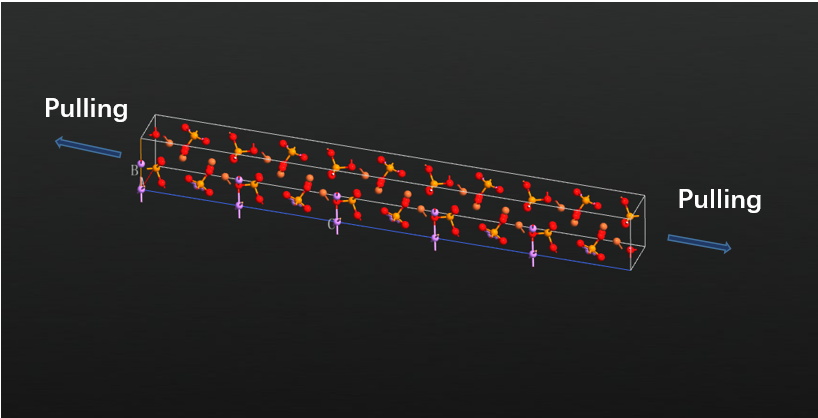
\includegraphics[width=\textwidth]{MD.png}
	\caption{$LiFePO_4$晶体的应力应变响应的分子动力学模拟} 
	\label{fig:md}
\end{figure}
\subsection{模拟过程和结果}
模拟的体系如图\ref{fig:md}所示,在两侧施加变形,进行体系弛豫,并统计出应力情况则可以得到应力-应变曲线。模拟结果见图\ref{fig:md_result}。需要注意的是,图中在起初时,随着应变增加,应力却出现了一个小的下降,这是因为起初的结构整体在z方向(图\ref{fig:md}所示的箭头方向)呈现一个压缩状态。可以看出,对于晶体C方向的加载,在较小应变的时候($<7\%$)均有很好的线性性,即满足线弹性材料的情形,在应变到一定值($7\%$前后),出现了断裂,此处应力值有一个明显的下降。由此可以说明,由于锂离子扩散所引起的活性材料的体积变化很容易引起颗粒的断裂乃至失效。可以做一个简单的估算,对于特征尺寸为$x$的晶体,如果产生$\delta x$的形变,则其体积变化为:
\begin{equation}
\Delta V = [(x+\delta x)^3 - x^3]/x^3 = (1+ \delta x/x)^3 -1
\end{equation}
而在本文的模拟中,假设可以取$\delta x/x = 0.07$,则求得$\Delta V=0.225$,也就是说大概可以承受$22.5\%$的体积变化而不发生断裂,而实际的电池循环过程中其体积变化却有可能超出这个范围\cite{Zhang2017Chemomechanical}。在图\ref{fig:md_result}中可以看出,锂离子嵌入和脱嵌会影响晶体的力学响应,具体而言,
锂离子嵌入使晶体的断裂应变减小。
\begin{figure}
	\centering   
	\includegraphics[width=\textwidth]{mdB.png}
	\includegraphics[width=\textwidth]{mdC.png}
	\caption{$LiFePO_4$晶体的应力应变响应及断裂行为的分子动力学模拟} 
	\label{fig:md_result}
\end{figure}

\section{总结和结论}
本章首先应用第一性模拟DFT方法求解锂离子沿着$LiFePO_4$晶体的两个方向扩散的扩散路径及其对应结构,并分别求出其势垒从而比较其扩散难易得出主要的扩散方向,这也同时可以通过对于化学反应速率的比较得出一致的结论。基于得到的扩散过程的结构,首先可以求出求弹性常数,从而可以进一步求出三个方向的杨氏模量和体弹模量乃至剪切模量,从而分析晶体力学特性在扩散过程中的变化。根据模拟和比较,锂离子的扩散行为和晶体的力学特性的耦合特性,在整个扩散过程中,杨氏模量会有最高$23\%$的减小。另外,通过分子动力学模拟的方法对于锂离子扩散前后的构型进行应变加载,统计测出其应力-应变曲线,并成功观测到了材料的断裂和塑性行为。在模拟中观测到在应变小于10\%时就会发生材料的断裂,而实际上所观测到的在循环过程中电极的体积膨胀所产生的应变要显著高于此值。研究发现,锂离子嵌入和脱嵌会影响晶体的力学响应,具体而言,锂离子嵌入使晶体的断裂应变减小。锂离子迁移引起的活性材料体积的变化很容易引起颗粒断裂,晶体在迁移前后有着不同的断裂力学响应
\\
\indent 在活性颗粒的层次,其力学行为和电化学特性密切相关。未来需要开展进一步诸如考虑电极老化等因素对于力学特性的影响;另外,进一步考虑胶层的作用将形成一个更加复杂的多界面、多层次的混合多物理场体系,对于这一体系的力学-电化学-热学特性的耦合研究需要进一步的开展。
\chapter{总结和展望}
\section{结果总结}
本研究对于锂离子电池活性层-集流体脱层失效行为进行了研究,对界面粘接强度进行了不同应变率状态下的混合拉伸-剪切实验,得到了锂离子电池力学建模中的界面力学参数。 研究发现:
\begin{itemize}
	\item 静态实验中,正极和负极的失效强度均在0.9$MPa$到2.4$MPa$之间,而相比之下,正极的强度要相对强于负极,这和正极的活性层的组成成分和涂布厚度有着直接关系。
	\item 动态加载下,正极和负极界面的断裂强度均有着显著的提升。以负极为例,相比静态实验中的断裂强度,其断裂强度在$0.1m/s$和$1m/s$速度加载下分别达到了$3.5MPa$和$3.8MPa$。
	\item 对正极而言,其活性层和集流体之间的剪切强度大致为拉伸强度的两倍,而对负极两者则大体相当。
	\item 随着加载角度的变化即应力加载加载状态的变化,断裂强度发生了复杂的变化,但是统一而言,在有着较大剪切分量的情况下界面粘接强度会有所上升。 另外,尽管断裂强度的增加在较低的加载速度($0.1m/s$)处接近了阈值,但是断裂强度随着加载角度的变化规律却显著地受到加载速度的影响。
\end{itemize}
\indent 另一方面,本文也对电池活性材料的重要成分$LiFePO_4$晶体在锂离子的扩散过程中的力学乃至电化学性质利用第一性原理模拟和分子动力学计算的方法进行了模拟研究,研究发现:
\begin{itemize}
	\item 对于B和C两个晶体方向的扩散研究发现,锂离子在B方向输运的能垒显著低于C方向的能垒(约为12\%),锂离子的输运有着极强的方向性。 
	\item 对于锂离子在输运过程中的晶体构型弹性常数的计算发现,锂离子的输运过程中晶体的力学性质有着显著的改变,其杨氏模量可以最高有23\%的减小。 同时,由于晶体的构型和锂离子输运的影响,其力学参数有很强的各向异性,并会随着输运过程的进行而变化。
	\item 对$LiFePO_4$晶体在扩散前后(不同SOC下)的应力-应变响应的分子动力学模拟表明,锂离子嵌入和脱嵌会影响晶体的力学响应。锂离子嵌入使晶体的断裂应变减小,同时,锂离子迁移引起的活性材料体积的变化很容易引起颗粒断裂,晶体在迁移前后有着不同的断裂力学响应。

\end{itemize}
\section{展望}
本文的工作还有一些不足,可以从以下方面改进:
\begin{enumerate}
	\item 界面力学测试中其强度结果有着10\%左右的离散分布,而对于动态试验其离散度则更大,进一步的实验希望能改进实验样品设计特别是夹具设计使得实验的重复性有更好的效果。
	\item 对于锂离子输运的模拟值进行了对于负极活性材料的初步模拟,而尚未考虑正极活性材料乃至考量整个活性材料-粘结剂-导电剂的分子体系,进一步的模拟希望能建立更加复杂的体系对于锂离子扩散过程中的力学性质进行研究。
\end{enumerate}
\indent 本文作者对于未来的工作研究的方向有一下几点展望:
\begin{enumerate}
	\item 本文分别从宏观实验和微观模拟的角度对于电极活性层内部的脱层断裂失效进行了测试和模拟研究,得到了详实的结果和数据。 本文的宏观实验数据可以给电池力学模型提供标定参数,但是所标定的模型往往是一个不基于电池实际组成的宏观力学模型,其在考虑多物理场的分析计算和对于电池内部诸多力学电化学过程的机理研究中显得力不从心。 在这一方面,未来可以尝试在满足一定的假设和边界条件下,直接用满足电池内部实际材料构成的微观或者介观的模型进行力学、化学乃至热学方面的建模,从而进行多物理场多尺度的耦合分析。
	\item 电池的胶接强度除了受到电池循环中锂离子的脱嵌和嵌入的影响,还必然会受到随着电池的老化而产生的一系列诸如气体产生等一系列物理化学过程的影响,对于电池工作循环中的实际特性表现和发展的研究中,如果能基于分子层次的模拟,建立微观模型,对于研究内部多物理过程的耦合乃至提升电池性能和指导电池设计都有着重要意义。
\end{enumerate}





%%% 其它部分
\backmatter

%% 本科生要这几个索引,研究生不要。选择性留下。
% 插图索引
\listoffigures
% 表格索引
\listoftables
% 公式索引
\listofequations


%% 参考文献
% 注意:至少需要引用一篇参考文献,否则下面两行可能引起编译错误。
% 如果不需要参考文献,请将下面两行删除或注释掉。
% 数字式引用
\bibliographystyle{thuthesis-numeric}
% 作者-年份式引用
% \bibliographystyle{thuthesis-author-year}
\bibliography{ref/refs}


%% 致谢
% 如果使用声明扫描页,将可选参数指定为扫描后的 PDF 文件名,例如:
% \begin{acknowledgement}[scan-statement.pdf]
\begin{acknowledgement}
  本科四年,午梦千山,窗阴一箭,其间在学习科研方面得到了很多老师的教诲和同学的帮助。首先要感谢课题组的周青老师,是周老师当年生动详实的讲座引发了我对汽车安全领域的浓厚兴趣,难以忘怀周老师给我们讲述自己如何是用一个十分简洁的力学模型做出了关于乘员头部碰撞防护的工作,也难以忘怀每一次和周老师交流时的侃侃而谈。 桃李不言,下自成蹊。 同时,也十分感谢课题组的夏勇老师,十分感谢夏老师的悉心指导,在我做毕业设计期间指导我对于这一领域有了初步的理解并使得我掌握了很多分析处理相关问题的能力。\\
  \indent感谢冯西桥老师的固体力学基础课程和许春晓老师的流体力学课程,在他们的课堂上我建立了关于经典力学体系的初步认识和系统概念。也十分感谢张雄老师的有限元基础和任玉新老师的计算流体力学基础,正是这两门数值模拟的课程让我掌握了力学建模的能力,能进一步对诸多问题进行尝试和研究。\\
  \indent在力学专业课程之外,十分感谢钱学森力学班对于课程灵活性的包容和鼓励,使我能学习一些自己感兴趣的课程,而这些课程也教会了我相当多的东西。最最令我难忘的是高研院徐湛老师开设的量子力学的课程,课堂上的精妙讲述,课堂下对于诸多问题的激烈讨论使得我深深地爱上了物理学,不仅仅是量子力学的美妙和神奇,徐老师的严谨治学和深刻思维给我至今依然是我心中的榜样。\\
  \indent 从大二开始在曹炳阳老师实验室做研究的两年时间是紧张而快乐的,每周三的组会对一个个问题的讲解和讨论使得我逐渐确立了一套自己的关于研究的体系性的看法。 其间,感谢实验室的华钰超师兄,带着我学会了声子蒙特卡洛模拟、第一性原理模拟的模拟方法,并在讨论中给我详细而有前瞻的指导。也感谢东京大学的鞠生宏师兄给予我的关于界面格林函数乃至相关优化算法的研究的指导。\\
  \indent 感谢东京大学Junichiro Shiomi教授,在实验室暑研期间,每次和教授的讨论,他总能把握问题的核心和关键,深厚的理论基础和丰富的科研经历,特别是那随手捻来的文献和独到深刻的见解都让我叹为观止。依稀记得,在最终的汇报中老师给我讲述了面对详实的数据给我讲述了不应该拘泥于分析工具而应该着眼于研究目标和物理本质的研究思路,我还依稀记得在和他讨论时他所说:
  \begin{quote}
   'You are the first one in the world to gain these data, but what you should care about is not only the application, for example, use ML to gain the Minimum ITC, I strongly recommend you that you should consider the physics using something like regression. You know, regression is a very old tool but you need remember regression can but the Machine Learning cannot tell you, is the physics. '
  \end{quote}
  \indent
  \indent感谢实验室潘哲鑫师兄给予我在实验方法和分析上的指导,感谢罗海灵师兄、陈冠华师兄给我在电池分析和建模上的指导。\\
  \indent感谢刘千惠同学和我讨论实验设计和建模分析的方法、以及图像分析的算法,最重要的是一直以来对我遇到困难和挫折的无尽支持和鼓励,当然还有每一天给我带来的快乐和欣喜。 我曾以为人生的意义在于四处游荡逃亡,但我如今已找到愿意驻足的地方。
  \\
  \indent 感谢我的父母一直以来的付出和对我的支持理解,他们总是给我最大限度的自由,坚定地支持我选择和做出的每一个决定。
  \\
  \indent 感谢和我一起度过这四年的酸甜时光的同学和朋友,是你们组成了我大学时光中最明丽的亮色。
  \\
  \indent感谢计算机系薛瑞尼同学提供的论文的Latex模板,给我论文的撰写提供了很大的方便。
  \\
  \indent 愿这篇论文成为审慎思考的起点,愿我能登高而望,星空璀璨。
  \\
  \indent 夢のある人が、周りに流されない。
  \\
  \indent 有梦想,你就不会随波逐流。
  \end{acknowledgement}


%% 附录
\begin{appendix}
%\chapter{文献调研报告}
%\label{cha:engorg}
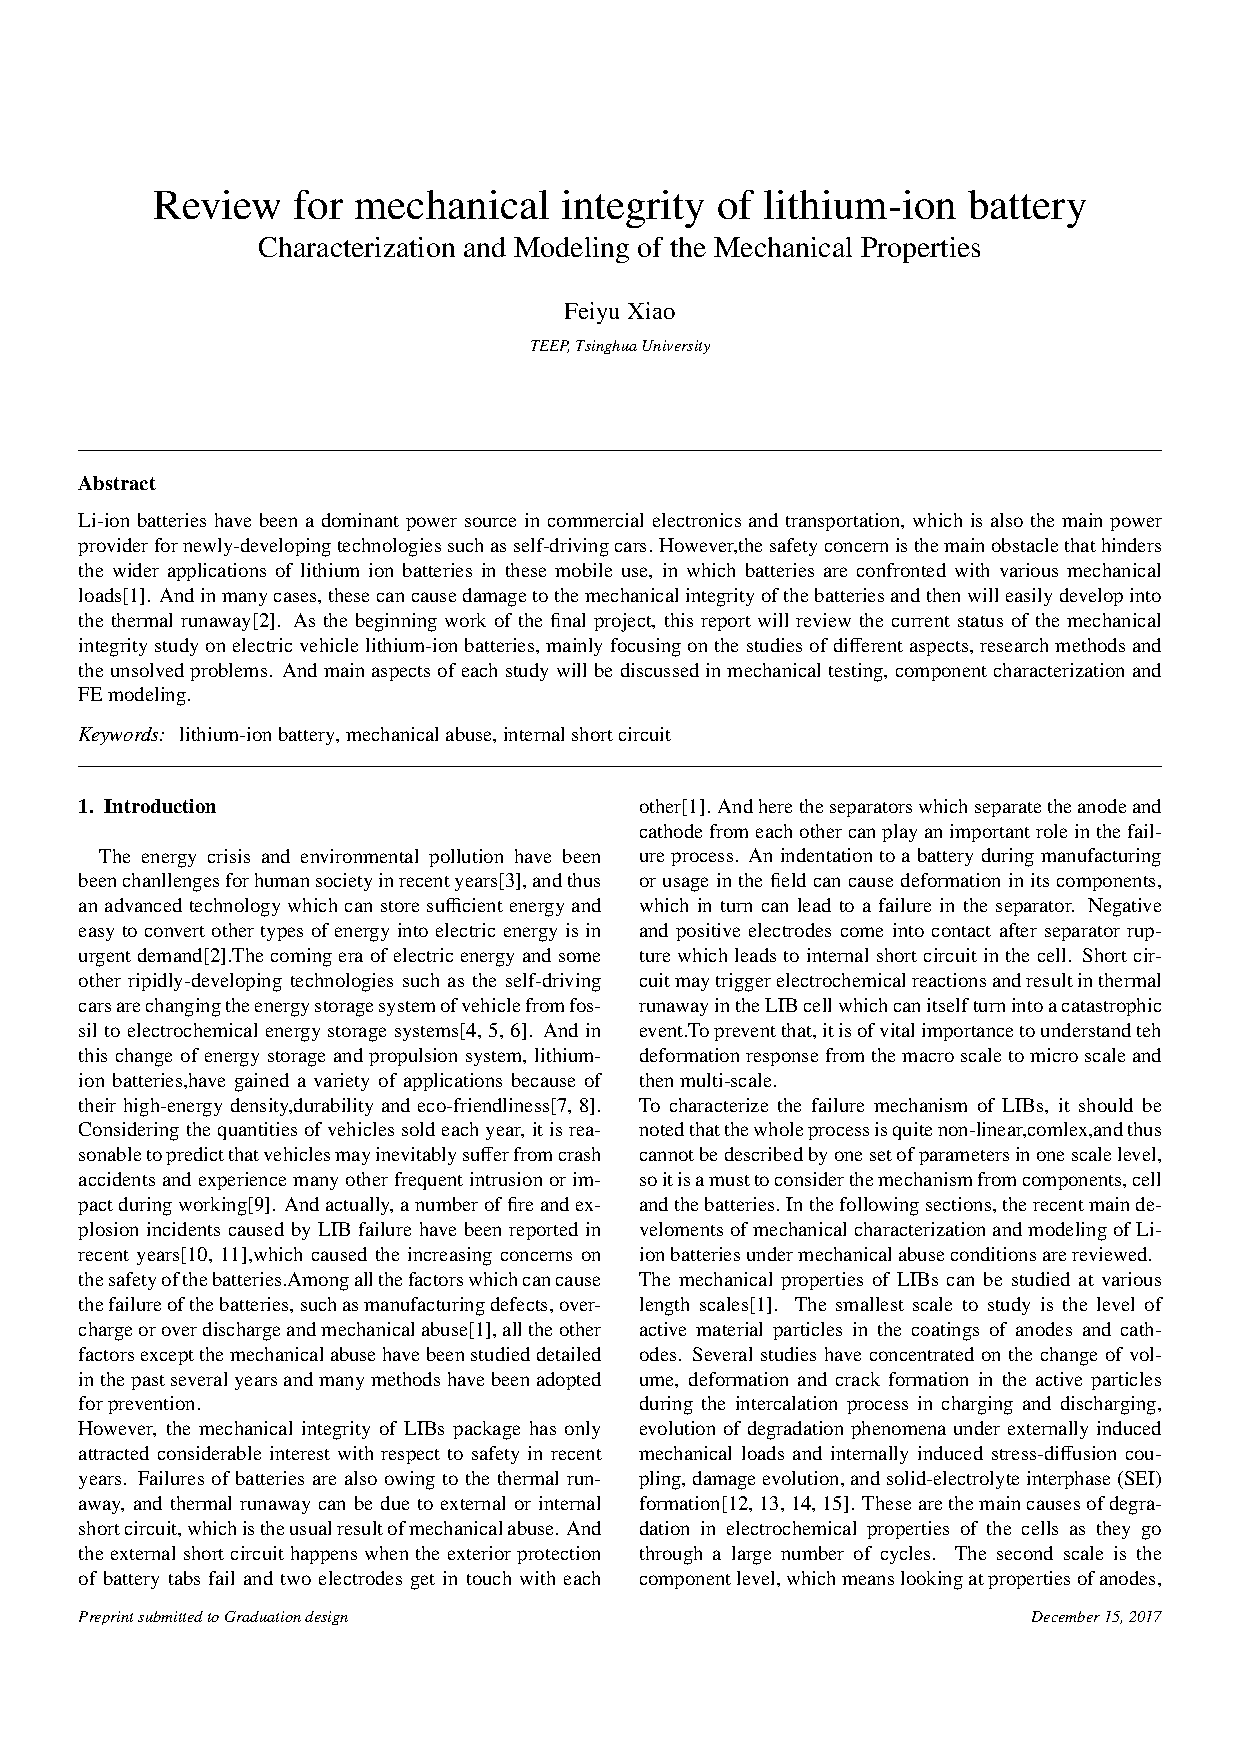
\includepdf[pages=-]{data/review.pdf}



\chapter{实验测试技术}
\section{Digital Image Correlation Measurements(DIC)}
DIC技术自从上个世纪八十年代被发明\cite{Sutton1983Determination}以来,作为一种非接触的基于数字灰度图像的全视野的图像分析方法,在确立物体的轮廓和位移方面得到了广泛的应用。\\
\begin{figure}
\centering   
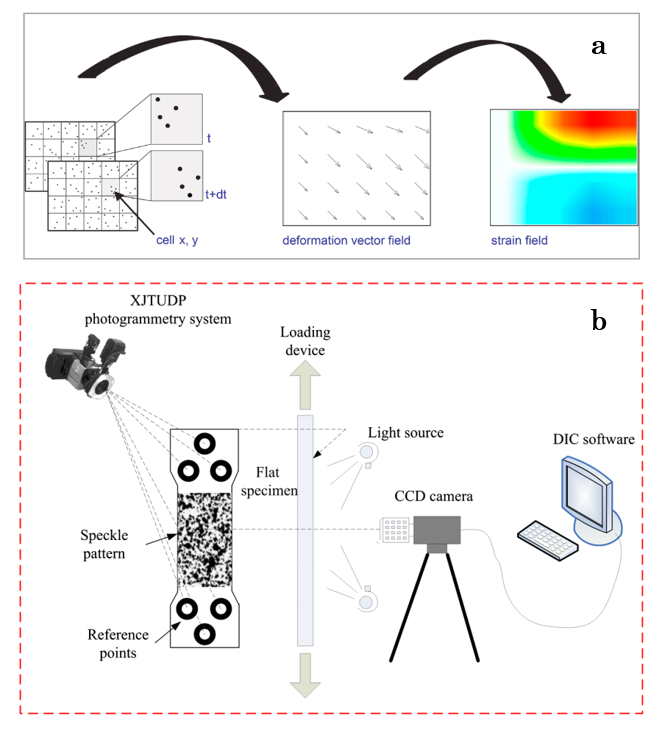
\includegraphics[width=0.8\textwidth]{DIC.png}
\caption{(a)DIC测量位移原理图(b)2D-DIC装置图\cite{Tang2012Photogrammetry}}
\label{fig:dic}
\end{figure}
\indent 如图\ref{fig:dic}(a)所示,DIC可以得到整个测试表面的位移和应变。其依据的原理是通过输入不同时刻的散斑图像进行比对,可以准确地得到全场的位移和应变输出(装置和流程图见图\ref{fig:dic}(b))。由于其全场同时测量和非接触测量的特性,DIC技术在包括实验力学在内的多个学科中发挥了重要作用。
\section{Energy Dispersive Spectrdmeter}
\begin{figure}
\centering   
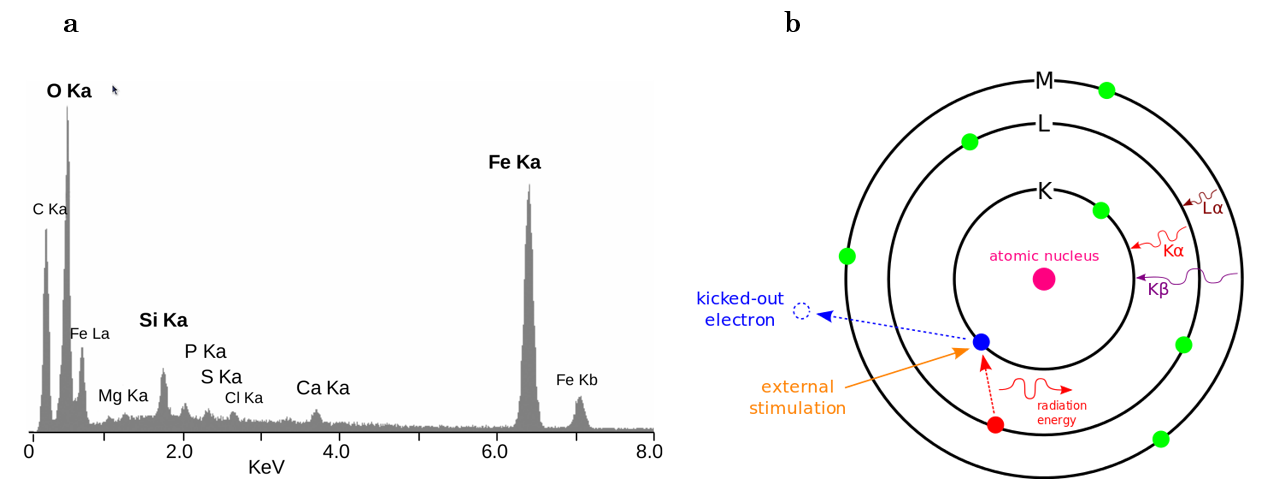
\includegraphics[width=\textwidth]{EDS_set.png}
\caption{(a)EDS频谱示意图\cite{L2008Iron}(b)EDS原理示意图\cite{wiki:eds}}
\label{fig:EDS}
\end{figure}
如图\ref{fig:EDS}所示,电子能谱分析方法的基本思路是利用单色性很好的高频率光源(如激光和X射线)集中照射待分析样品,使得样品表面的原子中的电子被激发到较高价态。 基于量子力学,处于不同量子态的电子其会有不同的动量、角动量乃至自旋的特征的不同分布\cite{Dirac1958The},从而测量这些电子的特征就可以得出材料的特性。\\
\indent 在本文的分析中,对于活性层的纵向切面进行了EDS分析,特别考察了Si元素沿着深度方向的分布情况,有力地佐证了实验测试方法的可行性和实验结果的科学性。
\chapter{分子模拟方法简介}
\section{密度泛函第一性原理计算}
\subsection{密度泛函理论简介}
密度泛函理论(Density function theory, DFT)是广泛应用在物理学,化学乃至材料科学中的一种依靠研究电子密度结构来对多粒子体系进行研究的方法。 在这一方法中, 多电子体系的性质可以依据电子密度泛函来决定,从而得名密度泛函。 这一理论实际上会通过一些合理的近似和假设,将实际包含着电子-电子相互作用的问题进行简化,化为无相互作用的体系的问题加以求解,并有着自己的一套控制误差的理论方法。\\
\indent 根据量子力学基本原理,只需要得到一个体系的波函数 $\Psi(r,t)$,就可以得到这个体系的全部信息,一般地利用波恩-奥本海默近似(忽略原子核的运动),一般体系的控制方程为下面的含时薛定谔方程:
\begin{equation}
\label{eq:sch}
\widehat{H} \Psi = \left[ \widehat{T} + \widehat{V} +\widehat{U} \right] \Psi = \left[ \sum^N_i \left( -\frac{\hbar^2}{2m_i} \nabla^2_i \right) + \sum^N_i V(\mathbf{r_i}) + \sum^N_{i < j} U(\mathbf{r_i},\mathbf{r_j}) \right] \Psi = E \Psi
\end{equation}
其中$\widehat{H}$为体系的哈密顿算符,T和V分别为动能算符和电场,而U电子-电子相互作用。 其实方程的难解在于U这一项十分复杂,比如大学物理中会给出解析解的氢原子和类氢原子能级的解,这是因为这些粒子没有电子的相互作用项。 而实际上绝大多数的体系都是有复杂的电子相互作用的因此得不到解析解,从而数值解在对于实际体系而言几乎是唯一的方法。\\
\subsubsection*{H-K定理}
\indent 在介绍密度泛函方法前,首先介绍其建立的基础:Hohenberg–Kohn theorems。
\begin{enumerate}
	\item H-K第一原理: 对于一个电子态密度 $n(\mathbf{r})$ 有着唯一对应的基态势能项$V_{ext}(\mathbf{r})$和基态总能量E,那么方程\ref{eq:sch}中的基态能量可以用电子密度表示为:
	\begin{equation}
	E[n(\mathbf{r})] = \Psi^{*} \left(
	\widehat{T} + \widehat{V} +\widehat{U} \right)
	\end{equation}
	此时,薛定谔方程的自由度从之前的N粒子对应的3N下降到了3,使得运算的复杂度大大降低。
	\item H-K第二定理:第二定理实际上是第一定理的变分原理,即能获得最低能量的电子密度即为基态电子密度。

\end{enumerate}
\subsubsection*{密度泛函理论基本框架}
基于H-K定理,体系的波函数$\Psi$和能量E以及体系的其他物理量都是电子态密度 $n$ 的函数。
首先,电子态密度可以用体系波函数表示为:
\begin{equation}
n = n(\mathbf{r}) = N \int d\mathbf{r_1} ... \int d \mathbf{r_N} \Psi^*(\mathbf{r},\mathbf{r_2},...,\mathbf{r_N})\Psi(\mathbf{r},\mathbf{r_2},...,\mathbf{r_N})
\end{equation}
体系总能量可以写成
\begin{equation}
E(n) = \Psi^*(n) \widehat{H} \Psi(n) = \Psi^*(n) \left(\widehat{T} + \widehat{U} + \widehat{V} \right) \Psi(n)
\end{equation}
此时,方程被简化为三个自由度,可以进行下一步的简化。
\begin{itemize}
	\item 动能项$\mathbf{T}$:\\
	忽略电子间相互作用,则动能项可以简化为:
	\begin{equation}
	T(n) \approx T_s(n) = -\frac{\hbar^2}{2m} \sum^{N}_{i=1} \int d^3r \Phi^*_i(\mathbf{r}) \nabla^2 \Phi_i(\mathbf{r})
	\end{equation}
	其中,$\Phi_i(\mathbf{r})$是第i个电子的轨道波函数,而$T_s(n)$为这些电子的轨道动能的和。
	\item 外势能项:\\
	依据波恩-奥本海默近似,可以得到外势能的表达式
	\begin{equation}
	V(n) = \int V(\mathbf{r}) n(\mathbf{r})d\mathbf{r}
	\end{equation}
	\item 相互作用:\\
	依据托马斯-费米模型得出一个很符合直觉的近似:
	\begin{equation}
	U(n) \approx U_{H}(n) = \frac{e^2}{2} \int d \mathbf{r} \int \mathbf{r'} \frac{n(\mathbf{r})n(\mathbf{r'})}{|\mathbf{r}-\mathbf{r'}|}
	\end{equation}
\end{itemize}
将上面三项求和可以得到能量的近似表达:
\begin{equation}
E_{approx}(n) = T_s(n) + U_H(n) + V(n)
\end{equation}
定义其和实际能量的差为交换-关联能(exchange-correlation energy):
\begin{equation}
\label{eq:e}
\varepsilon = (T - T_s)+(U - U_H) = E_{XC}
\end{equation}
\subsubsection*{交换-关联泛函}
根据上面的陈述可以发现其实DFT的核心在于如何计算上面的\ref{eq:e},这就有诸如局域密度近似(LDA)和广义梯度近似等方法。由于在本文的研究中,所关注的是锂离子的扩散,其电子密度改变相对不是很快,于是可以选择计算难度较小的LDA方法。\\
局域密度近似(Local Density Approximation, LDA)\\
\indent LDA近似认为空间各个点的$E_{XC}$即交换-交联能只和该点出的电子密度有关,这一关键假设决定其本质上是一个局域的理论,在对于主要是短程相互作用的体系这一简化就十分有力。 LDA的表达式可以写为:
\begin{equation}
E^{LDA}_{XC}(n) = \int d \mathbf{r} \mathnormal{f}(n)
\end{equation}
对于$E_{XC}$其可以自然地被分为两部分(交换和关联项):
\begin{equation}
E^{LDA}_{XC} = E^{LDA}_X + E^{LDA}_C
\end{equation}
\begin{enumerate}
	\item 其中的交换部分可以使用均匀电子近似假设予以简化,得到其交换能(用狄拉克泛函给出)为:
	\begin{equation}
	E^{LDA}_X(n) = -\frac{3}{4} \left(\frac{3}{\pi} \right)^{1/3} \int d^3r n(\mathbf{r})^{4/3}
	\end{equation}
	\item 而对于关联部分,分为高密度和低密度下有着两种近似方法:
	\begin{itemize}
		\item 高密度情况下,对于空间点的关联能为:
		\begin{equation}
		\varepsilon_C = Aln(r_s) + C + \mathnormal{O}(r_s)
		\end{equation}
		其中$r_s = \frac{1}{a_0} \left(\frac{3}{4\pi n} \right)^{-3}$。
		\item 对于低密度情况,可以将空间某点关联能写为:
		\begin{equation}
		\varepsilon_C = \frac{1}{2} \left(\frac{g_0}{r_s} + \frac{g_1}{r^{3/2}_s} + ... \right) \quad g_0 \approx -0.884,\quad g_1=3
		\end{equation}
	\end{itemize}
\end{enumerate}
(本节所主要参考的文献为\cite{Parr1989Density,Burke2005Time,Becke1993Density})
\subsection{锂离子扩散过程模拟方法——微动弹性带方法}
在本文的模拟过程中,其中的一个关键的难点是如何根据锂离子扩散前后的构型得到扩散过程中的亚稳定构型,从而对扩散过程中的晶体力学性质展开研究。在模拟中,本文采用微动弹性带的方法寻找初始和最终构型间的能量的鞍点并得到最小能量路径。这一方法会在保证每个中间构型的最低能量的同时去保证过程之间的能量差的平衡。 其实际的优化是通过在不同能层之间添加弹簧力从而得到垂直于带的投影力的分量来进行。实际的操作是对于一系列可能构像,附加上除了化学力之外的弹簧力,然后让优化算法进行约束构象间隔的弛豫,每一个点的作用力都可以写成下列形式:
\begin{equation}
\mathbf{f}_i = \mathbf{f}^{\parallel}_i - \mathbf{g}^{\perp}_i
\end{equation}
其中
\begin{equation}
\mathbf{f}^{\parallel}_i = k \left[(\mathbf{r_{i+1}} - \mathbf{r_i}) - (\mathbf{r_i} - \mathbf{r_{i-1}}) \times \tau_i \right]\tau_i
\end{equation}
是弹簧力沿着构象路径的分量。
\subsubsection*{Climbing Image Method}
为了更加精确的模拟锂离子的扩散,在NEB方法的基础上可以引入一个小的修正,这也是本文在模拟中所实际采用的方法。具体是将最高能量的构想驱动到鞍点,然后在这里不施加弹簧力,将沿着切向的真实体系里倒置进行优化。从而可以使得整个构想会最大限度的沿着频带的切向发展,而在其他的所有方向最小化,知道收敛时所达到的鞍点会更加精确。\\
(本节的主要参考文献为\cite{Henkelman2000Improved,Henkelman2000A,Smidstrup2014Improved})
\subsection{化学反应率计算——谐波过渡态理论}
本文在模拟锂离子在$LiFePO_4$晶体中沿着不同方向扩散的能垒时还计算了其分别的化学反应率,其计算理论和方法为谐波过渡态理论(Harmonic Transition State Theory,HTST),此处对这一方法做一个简要介绍。
对于化学反应行为的模拟,原则上可以采用下一节将会介绍的分子动力学模拟的方法,但是往往在固体中的化学反应比较缓慢从而使得分子动力学的迭代耗费十分巨大,此时另辟蹊径从统计力学的角度出发进行计算不失为一种很好的解决思路。\\
\indent 谐波过渡态方法通过从化学反应的产物中推测出反应物的过渡态来进行分析。对于固体中的反应而言,采用谐波近似往往是十分有效的,另外往往系统的平均动能要比能量势垒小很多。\\
\indent 第一步是找到反应的鞍点,这其实可以通过之前所提到的Climb Image Method得到,而一旦到达鞍点就可以进行反应速率的计算:
\begin{equation}
K_{HTST} = \frac{\Pi^{3N}_{i} \nu^R_i}{\Pi^{3N-1}{i} \nu^S_i} exp \left[-(E^S -E^R)/k_bT\right]
\end{equation}
其中,$N$为原子数目,$\nu^R_i$和$\nu^S_i$为起始和鞍点构像的模态频率,$E^R$和$E^S$是最小点和鞍点的能量,$k_B$是玻尔兹曼常数。\\
值得指出的是,HTST的计算方法和著名的阿伦尼乌斯方程十分相似:
\begin{equation}
k_{Arr} = A exp\left[-E_a/k_BT\right]
\end{equation}
对于阿伦尼乌斯方程,其系数因子,A,相当于对应振动模态的乘积和在HTST方程中鞍上稳定振动模式乘积的最小值的比值,这可以看做是系统每秒沿着反应方向振动的次数。 同时,方程中的活化能,$E_a$是HTST中鞍点和最小能量之间的差异。 采用指数分布是因为沿着反应方向的振动会遵从玻尔兹曼分布,而后者正好是指数分布。\\
(本节的主要参考文献为\cite{Vineyard1957Frequency,Eyring1935The,Voter1984Transition})
\section{分子动力学}
分子动力学是研究原子和分子的运动从而得出体系特性的经典模拟方法。在分子动力学模拟中,粒子在模拟时间和模拟尺度内进行相互作用,从而进行运动和重新分布,进而给出系统随着时间动态演化的信息。 通常而言,对于经典的分子动力学,其通常采用粒子间的给定的势场来得到粒子间的相互作用力,从而求解相互作用系统的牛顿方程从而得到粒子的运动轨迹。\\
\indent 对于通常的多粒子体系而言,其组成系统的粒子总数通常是非常之多的,从而应用通常的方法进行系统性质的分析就十分的困难,而恰恰分子动力学方法可以依靠统计力学和数值积分的方法比较好的解决这一难点。 对于一个满足各态历经假设的系统,就可以采用分子动力学模拟来确定系统的宏观热力学性质——即遍历系统的时间平均值对应微正则系综平均值。 从而,分子动力学手段可以通过统计力学的原理来洞察到系统在原子尺度的发展演变。
\\
\indent 要进行分子动力学模拟,需要预先给定势函数和系综方法,势函数可以从化学结构如化学键的研究得到,也可以通过量子力学的模拟和计算得到,关于势能的选取前文部分有详细的说明,此处不再赘述,以下将对系综方法进行简要介绍。\\
\indent 对于统计力学而言,其求得宏观物理量的方法是对微观状态求统计平均。而实际上,分子的动量和能量的交换十分的频繁和剧烈(如1s中可以发生$10^{28}$次碰撞),在相空间中系统的微观状态十分迅速地发生着变化。这也就意味着想对宏观系统(包含$10^{23}$以上粒子)的哈密顿方程进行积分求解是完全没有可能的,而系综正是将对时间上的平均变换为对微观状态的平均,其本质为将牛顿力学转换为统计规律。 假设可以复制出有着完全一样的宏观约束参数的系统,其显然可以处于不同的微观状态,而这些尽可能多的系统每一个都实际上等价于相空间中的一个点,从而这些系统整体构成了一个系综(Ensemble)。而对于不同的约束条件,自然就区分为不同的系综:
\begin{itemize}
	\item 正则系综(Canonical Ensemble, NVT)\\
	假设N个粒子在体系为V的系统中,其环境为温度恒定为T的热浴。那么总能量和系统的压强可能在一个稳定值附近波动,此时系统有特征函数亥姆霍兹自由能$\mathcal{H}(N,V,T)$可以用来求得所有宏观物理参数。
	\item 微正则系综(Micro-Canonical Ensemble,NVE)\\
	微正则系综被广泛应用在分子动力学模拟中,假定N个粒子处于体积为V的系统中,给定总能量E,此时温度和压强均可能产生波动,系统的特征函数为熵$\mathcal{S}(N,V,E)$
	\item 等温等压系综(Constant-Pressure and Constant Temperature,NPT),即具有给定的粒子数,压强和温度,从而能量和体积会发生改变,特征函数是吉布斯自由能$\mathcal{G}(N,P,T)$。这一系综实际上是系统的边界可以发生移动的情况下给定环境为恒温的热浴的系综,也是本文在模拟$LiFePO_4$晶体在受到外载形变行为所采用的方法。
\end{itemize}
最后介绍分子动力学模拟的主要步骤和思路:
\begin{enumerate}
	\item 给定系统粒子初始的位移$\mathbf{r}^{i=0}$和速度$\mathbf{v}^{i=0}$,设定加速度$\alpha$初始值为零,并给定合适的时间间隔$\Delta t$
	\item 预测求出新的原子位形:给定原子位置 $\mathbf{r}^p = \mathbf{r}^{(i)}+ \mathbf{v}^{(i)} + 1/2 \alpha \Delta t^2 ...$ 更新原子速度 $\mathbf{v}^p = \mathbf{v}^{(i)}+\alpha \Delta t$
	\item 求出新的粒子受力$\mathbf{F} = - \nabla V(\mathbf{r}^p)$  或 $\mathbf{F} = \mathbf{F}( \Psi(\mathbf{r}^p))$ 继而求得加速度$\alpha = \mathbf{F}/m$
	\item 再应用新求得的加速度调整粒子的位形,即
	$\mathbf{r}^{i+1} = \mathbf{r}^p + \mathnormal{f}(\mathbf{a}, \Delta t)$和$\mathbf{v}^{i+1} = \mathbf{v}^p + \mathnormal{g}(\mathbf{a}, \Delta t)$
	\item 考察边界条件,比如控制温度压强(NVT)
	\item 计算宏观物理参数
	\item 继续迭代 $t=t+ \Delta t$,$i=i+1$
	\item 考察迭代次数,如果不满足终止条件,继续从步骤1开始重复
\end{enumerate}
(本节的主要参考文献为\cite{Frenkel1997Understanding,Rapaport2004The,Berendsen1998Molecular,Swope1982A})


\end{appendix}

%% 个人简历


\resumeitem{个人简历}

1997 年 2 月 3 日出生于陕西省汉中市。

2014 年 9 月考入清华大学航天航空学院工程力学系钱学森力学班,2018 年 7 月本科毕业并获得工学学士学位。





  

\researchitem{} 

I would like to dedicate this thesis to the respectful physicist and pioneer Dirac, whose book of Quantum Mechanics led me to the universe of science and more importantly the way how should I think over the miracle and explore the unknown of the world  . And I would like to quote a paragraph of his interview\footnote{T. Kuhn, interview with P.A.M. Dirac, 6 May 1963-Tape 62b, Niels Bohr Library, American Institute of Physics, New York.} which is an abstract of my principles:
\textit{I owe a lot to my engineering training because it taught me to tolerate approximations. Previously to that I thought...one should just concentrate on exact equations all the time. Then I got the idea that in the actual world all our equations are only approximate. We must just tend to greater and greater accuracy. In spite of the equations being approximate, they can be beautiful.}





%% 本科生进行格式审查是需要下面这个表格,答辩可能不需要。选择性留下。
% 综合论文训练记录表
%\includepdf[pages=-]{scan-record.pdf}
\end{document}
